\documentclass[defaultstyle,10pt,master]{01.thesis}

%% Packages
\typeout{}
\typeout{--------------------------------------------------------------}
\typeout{ +---+ Thesis Template                            }
\typeout{ +---+      Version 2.0, August 2011                         }
\typeout{ +---+  for Instituto Superior Tecnico (IST),                 }
\typeout{ +---+  Universidade T�cnica de Lisboa                         }
\typeout{ * Using Thesis Style form Pedro Tom�s                                }
\typeout{ * Created to write Dissertations                             }
\typeout{ * Conforms with IST Master Degree format and with most important packages setup        }
\typeout{ * Should conform with IST PhD Degree format (not verified)   }
\typeout{                                                              }
\typeout{ AUTHOR: Miguel Amador and Jo�o Marques                                          }
\typeout{                                                              }
\typeout{Important: Use all files in the archive, since this is based in all them. Modify dummy files at wish.                                                              }
\typeout{--------------------------------------------------------------}
\typeout{}

% Defines an additional alphabet... not required in most cases
% ------------------------------------------------------------
% \DeclareMathAlphabet{\mathpzc}{OT1}{pzc}{m}{it}

% PACKAGE babel:
% ---------------
% The 'babel' package may correct some hyphenisation issues of latex. 
% However in most situations it is not required.
\usepackage[english]{babel}

% PACKAGE fontenc:
% -----------------
% chooses T1-fonts and allows correct automatic hyphenation.
%\usepackage[T1]{fontenc}
\usepackage[latin1]{inputenc}

% Package ulem.
\usepackage{ulem} % Allows the use of other text emphatizer commands
\normalem %defines \emph{} to italic, instead of underline. 
\raggedbottom %declaration makes all pages the height of the text on that page. No extra vertical space is added. The \flushbottom declaration makes all text pages the same height, adding extra vertical space when necessary to fill out the page.

% PACKAGE date time:
% -----------------
% Lets you alter the format of the date that \today returns.
\usepackage{datetime}
\newdateformat{todaythesis}{%
\monthname[\THEMONTH]  \THEYEAR}

% PACKAGE latexsym:
% -----------------
% Defines additional latex symbols. May be required for thesis with many math symbols.
\usepackage{latexsym}

% PACKAGE amsmath, amsthm, amssymb, amsfonts:
% -------------------------------------------
% This package is typically required. Among many other things it adds the possibility
% to put symbols in bold by using \boldsymbol (not \mathbf); defines additional 
% fonts and symbols; adds the \eqref command for citing equations. I prefer the style
% "(x.xx)" for referering to an equation than to use "equation x.xx".
\usepackage{amsmath, amsthm, amssymb, amsfonts, amsbsy}

% PACKAGE multirow, colortbl, longtable:
% ---------------------------------------
% These packages are most usefull for advanced tables. The first allows to join rows 
% throuhg the command \multirow which works similarly with the command \multicolumn
% The second package allows to color the table (both foreground and background)
% The third package is only required when tables extend beyond the length of one page;
% with compatibilities with the tabular environment. The last allow the definitions of landscape pages, allowing the use of a different orientation for wider graphics or tables. See package documentation to see the implementation.
\usepackage{multirow}
\usepackage{colortbl}
\usepackage{supertabular}
\usepackage{pdflscape}
\usepackage{longtable}

% PACKAGE graphics, epsfig, subfigure, caption:
% ---------------------------------------------
% Packages for figures... well you will certainly need these packages, with the exception
% of the 'caption' package. This only allows to define extra caption options.
% Notice that subfigure allows to place figures within figures with its own caption. It
% should be avoided to create an eps file with subfigures. That will mean that you won't be 
% able to reference those subfigures. Instead create an EPS file (the only graphics format supported
% by latex) for each of the subfigures and then use the command \subfigure (see below).
\usepackage{graphics}
\usepackage{graphicx}
\usepackage{epsfig}
\usepackage[hang,small,bf]{subfigure}
%\usepackage[footnotesize,bf,center]{caption}
\usepackage{dcolumn}
\usepackage{bm}
\usepackage{booktabs}
\usepackage{rotating}
\usepackage{multirow}

\usepackage[font=small,labelfont=bf,textfont=normalfont]{caption}

% PACKAGE algorithmic, algorithm
% ------------------------------
% These packages are required if you need to describe an algorithm.
% \usepackage{algorithmic}
% \usepackage[chapter]{algorithm}

% PACKAGE natbib/cite
% -------------------
% The two packages are not compatible, and you should use one of the two. Notice however that the
% IEEE BiBTeX stylesheet is imcompatible with the natbib package. If using the IEEE format, use the 
% cite package instead
\usepackage[]{natbib}
%\usepackage[square,numbers,sort&compress]{natbib}
%\usepackage{cite}
\usepackage{bibentry}

% PACKAGE acronyum
% -----------------
% This package is most useful for acronyms. The package guarantees that all acronyms definitions are 
% given at the first usage. IMPORTANT: do not use acronyms in titles/captions; otherwise the definition 
% will appear on the table of contents.
\usepackage[printonlyused]{acronym}
\usepackage[titletoc,title,header]{appendix}
\usepackage[noauto]{chappg}

% PACKAGE extra_functions VER COMO DEVE SER
% -----------------
% My Personal package: defines the following commands:
% \fancychapter{chaptername) -> Prints a fancier chapter (you can also use the fancychapter package for this)
% \hline{width} -> use for a replacement of the \hline command
% \Mark1, \Mark2, \Mark3, ...
\usepackage{00.extra_functions}


% PACKAGE hyperref
% -----------------
% Set links for references and citations in document
% Some MiKTeX distributions have faulty PDF creators in which case this package will not work correctly
% Long live Linux :D
\usepackage[plainpages=false,hidelinks]{hyperref}
\hypersetup{
             colorlinks=false,
             citecolor=white,
             breaklinks=true,
             bookmarksnumbered=true,
             bookmarksopen=true,
             pdftitle={Numerical modelling of fully coupled solid-fluid flows},
             pdfauthor={Ricardo Birjukovs Canelas},
             pdfsubject={PhD Thesis in Civil Engineering},
             pdfcreator={Ricardo Birjukovs Canelas},
             pdfkeywords={Template, Latex, Thesis}}
\usepackage{float}
%\usepackage[final]{00.listofsymbols}
\usepackage{00.symlist}

% Set paragraph counter to alphanumeric mode
\renewcommand{\theparagraph}{\Alph{paragraph}~--}

\newcommand{\figref}[1]{Figure \ref{#1}}
\newcommand{\equationref}[1]{Equation (\ref{#1})}
\newcommand{\tableref}[1]{Table (\ref{#1})}

\newcommand{\ve}[1]{\boldsymbol{#1}}

\newcommand{\textreg}{$\textsuperscript{\textregistered}$}

\usepackage[export]{adjustbox}

%%%%%TO USE EPS WITH PDFLATEX - BRILIANT %%%%%%
\newif\ifpdf
\ifx\pdfoutput\undefined
   \pdffalse
\else
   \pdfoutput=1
   \pdftrue
\fi
\ifpdf
   \usepackage{graphicx}
   \usepackage[update]{epstopdf}
   \DeclareGraphicsRule{.eps}{pdf}{.pdf}{`epstopdf #1}
   \pdfcompresslevel=9
\else
   \usepackage{graphicx}
\fi

%% Page formatting
\hoffset 0in
\voffset 0in

%Alternative set of page geometry
%\oddsidemargin 0.71cm
%\evensidemargin 0.04cm
%\marginparsep 0in
%\topmargin -0.25cm
%\textwidth 15cm
%\textheight 23.5cm

\usepackage[top=2.5cm, bottom=2.5cm, inner=2.9cm, outer=2.5cm]{geometry}

\usepackage{fancyhdr}
\pagestyle{fancy}
\renewcommand{\chaptermark}[1]{\markboth{\thechapter.\ #1}{}}
\renewcommand{\sectionmark}[1]{\markright{\thesection\ #1}}
\fancyhf{} 
%\fancyhead[LE]{\bfseries\nouppercase{\leftmark}}
%\fancyhead[RO]{\bfseries\nouppercase{\rightmark}}
\fancyfoot[LE,RO]{\bfseries\small\thepage}
\renewcommand{\headrulewidth}{0.0pt}
\renewcommand{\footrulewidth}{0.0pt}
\addtolength{\headheight}{2pt} % make space for the rule
\fancypagestyle{plain}{% Used in Chapter titles
   \fancyhead{} % get rid of headers
   \renewcommand{\headrulewidth}{0pt} % and the line
   \renewcommand{\footrulewidth}{0pt}
   \fancyfoot[LE,RO]{\bfseries\small\thepage}
}

\fancypagestyle{begin}{%
   \fancyhead{}
   \renewcommand{\headrulewidth}{0pt}
   \renewcommand{\footrulewidth}{0pt}
   \fancyfoot[LE,RO]{\bfseries\small\thepage}
}
\fancypagestyle{document}{%
	\fancyhf{} 
	\fancyhead[LE]{\bfseries\nouppercase{\leftmark}}
	\fancyhead[RO]{\bfseries\nouppercase{\rightmark}}
	\fancyfoot[LE,RO]{\bfseries\small\thepage}
	%\renewcommand{\headrulewidth}{0pt}
	%\renewcommand{\footrulewidth}{0pt}
	\addtolength{\headheight}{2pt} % make space for the rule
}
\fancypagestyle{documentsimple}{%
	\fancyhf{}
	\fancyfoot[LE,RO]{\bfseries\small\thepage}
	%\renewcommand{\headrulewidth}{0pt}
	%\renewcommand{\footrulewidth}{0pt}
	\addtolength{\headheight}{2pt} % make space for the rule
}
\setcounter{secnumdepth} {5}
\setcounter{tocdepth} {5}
\renewcommand{\thesubsubsection}{\thesubsection.\Alph{subsubsection}}

\renewcommand{\subfigtopskip}{0.3 cm}
\renewcommand{\subfigbottomskip}{0.2 cm}
\renewcommand{\subfigcapskip}{0.3 cm}
\renewcommand{\subfigcapmargin}{0.2 cm}

\graphicspath{{Figures/}}



%-----------------------------------------------------------
%-----------------------------------------------------------

\begin{document}
%\pagestyle{begin}
%\setcounter{page}{1} \pagenumbering{Alph}

% Add PDF bookmark 
\pdfbookmark[0]{Title}{Title}

\thispagestyle{empty}
\begin{flushleft} ~\\ \vspace{-10mm} \hspace{-1mm}  
\includegraphics[height=20mm]{Cover/IST_A_RGB_POS} %\hspace{35mm}
%
\includegraphics[height=10mm]{Cover/uvigo}
\center 
\LARGE \textbf{UNIVERSIDADE DE LISBOA}\\
\LARGE \textbf{INSTITUTO SUPERIOR T�CNICO}\\
%%\LARGE \textbf{UNIVERSIDADE DE VIGO}
%\\ \vspace{1mm} % gr�ficos
%\\ \begin{center} %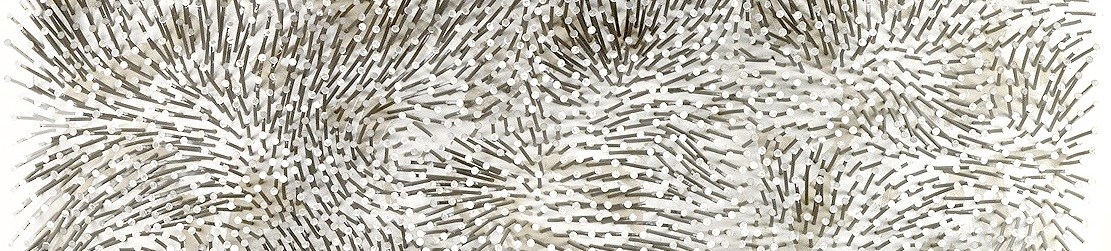
\includegraphics[width=0.90\linewidth]{Cover/Uecker_II_small}  \end{center} % gr�ficos
\begin{centering}
%\small G\"unther Uecker, \emph{1987}\\
\vspace{15mm}
\LARGE \textbf{Numerical modeling of fully coupled solid-fluid flows}
\\ \vspace{10mm}
\Large \textbf{Ricardo Jorge Fonseca Birjukovs Canelas}
\\ \vspace{10mm}
\begin{tabular}{lcl}
\large \textbf{Supervisor}:		& \large \textbf{Doctor Rui Miguel Lage Ferreira}  &  \\ 
\large \textbf{Co-Supervisor}: 		& \large \textbf{Doctor Ram�n G�mez-Gesteira}  &  \\
\end{tabular}
\vspace{10mm}

\large \textbf{Thesis approved in public session to obtain the PhD Degree in Civil Engineering}\\
\vspace{5mm}
\large {{Jury final classification: Pass with Distinction}} \\
\vspace{10mm}

\large \textbf{Jury}\\
\end{centering}

\begin{flushleft}
 \large \textbf{Chairperson: Chairman of the IST Scientific Board}    \\
\vspace{2mm}\large \textbf{Members of the Committee}:  \\
\normalsize \textbf{Doctor Jo\~{a}o Gouveia Apar\'{i}cio Bento Leal}, Professor, Faculty of Engineering and Science, University of Agder, Norway   \\  
\normalsize \textbf{Doctor Ramon G\'{o}mez-Gesteira}, Professor Catedr�tico de la Faculdad de Ciencias, Universidad de Vigo, Spain  \\
\normalsize \textbf{Doctor Ramiro Joaquim de Jesus Neves}, Professor Associado do Instituto Superior T�cnico, Universidade de Lisboa  \\
\normalsize \textbf{Doctor Alejandro Jacobo Cabrera Crespo}, Investigador de la Faculdad de Ciencias, Universidad de Vigo, Spain \\
\normalsize \textbf{Doctor Rui Miguel Lage Ferreira}, Professor Auxiliar do Instituto Superior T�cnico, Universidade de Lisboa  \\
\normalsize \textbf{Doctor Carlos Manuel Tiago Tavares Fernandes}, Professor Auxiliar do Instituto Superior T�cnico, Universidade de Lisboa  \\
\end{flushleft}

\vspace{5mm}

\Large \textbf{Funding Institutions}\\
\vspace{2mm}
\large \textbf{Funda\c{c}\~{a}o para a Ci\^{e}ncia e Tecnologia} - FCT (SFRH/BD/75478/2010)\\
\large \textbf{Funda\c{c}\~{a}o para a Ci\^{e}ncia e Tecnologia} - FCT (PTDC/EMC/117660/2010)\\
\large \textbf{Funda\c{c}\~{a}o para a Ci\^{e}ncia e Tecnologia} - FCT (RECI/EMC-HID/0371/2012)\\

\vspace{5mm}
%\Large \textbf{\todaythesis\today} \\
\Large {\textbf{2015}} \\
\let\thepage\relax
\end{flushleft}
\pagebreak


\clearpage
% Since I am using double sided pages, the second page should be white.
% Remember that when delivering the dissertation, IST requires for the cover to appear twice.

\thispagestyle{empty}
\cleardoublepage

\setcounter{page}{1} \pagenumbering{roman}

\baselineskip 18pt % line spacing: -12pt for single spacing
                   %               -18pt for 1 1/2 spacing
                   %               -24pt for double spacingnts}
%\thispagestyle{empty}
\hbox{} \vfill
\begin{flushright}
\small \textit{\textbf{Remember that all models are wrong; the practical question is how wrong do they have to be to not be useful.}}
\\ \vspace{2mm}  
\scriptsize George E.P. Box and Norman R. Draper, Empirical Model-Building and Response Surfaces (1987)
\end{flushright}

\clearpage
\thispagestyle{empty}
\cleardoublepage
%
\pdfbookmark{Acknowledgments}{Acknowledgments}
\begin{acknowledgments} 

Existe muito por que estar grato aos meus pais. O sacrif\'{i}cio e a alegria com que o cometeram, as longas horas a lidar com uma mente incassi\'{a}vel, o ninho sempre pronto a que recorrer quando o mundo se demonstrou demasiado ventoso. A v\'{o}s. 

Ao Lu\'{i}s e Ana, pela infind\'{a}vel disponibilidade, pelo genu\'{i}no interesse, pelo carinho sem fim. A v\'{o}s.

Ao meu irm\~{a}o Diogo, pela presen\c{c}a e apoios constantes quando os dias assim o pedem. Pelas conversas, discuss\~{o}es e olhares de muitos anos de cumplicidade, a ti.

Aos meus tios, pelo sempre presente sorriso, boa disposi\c{c}\~{a}o e \'{o}ptimos conselhos de viagem. Pelo incondicional amor e disponibilidade com que sempre me presentearam.

I have been fortunate enough to share the stimulating working environments of two research groups. In all of CEris, I would like to thank particularly Ana Margarida, for proudly sharing the same space with someone as dubious as a numerics researcher. Daniel Conde for always being ready to defend the said numerics researcher, besides sharing my pains with compilers. To Artur Silva, for always bringing a new perspective, and particularly good 7th art recommendations. To Pedro Sanches, for transforming my descents into the pits of physical experimentation into highly enjoyable moments. I would also like to acknowledge Dulce Fernandes, Nuno Martins, Ana Quaresma, Rui Aleixo and Luis Mendes.

Part of my work was developed in UVigo, at EPHYSLAB, Ourense. Alejandro Crespo deserves special acknowledgment for the sheer effort to make me feel welcome and part of the team. Alex employed the full extend of his availability and critical approach to promote this work to a better level. He also took the entire team to the thermal baths whenever possible, in a great contribution towards the understanding of fluid mechanics. Jos\'{e} Domingu\'{e}z shared many hours looking at code and compiler warnings. I am ever so thankful to him, knowing that he made this work possible by helping me express my ideas within the computational maze that the project grew into. Anxo Barreiro, I will never forget that couch. A very big thank you to Angel Fernandez, Fran Santos, Orlando Feal, Xurxo, Corrado Altomare and Carlos Alvarado.

Behind a PhD there is always a well of vision, experience and support. I had two, Rui Ferreira and R\'{a}mon G\'{o}mez-Gesteira, my advisors. To both, I need to acknowledge the great opportunities that I was presented with. The amount of knowledge, patience and dedication devoted to this project make me proud, humbled and thankful. 

To FCT, for supporting the program with a full PhD scholarship, a fundamental requisite for its development.

To Olya, my wife, confidant and everything positive one can be to another. For sharing everything, for transmuting the good into sublime and the bad to part of the good. For the endless monologues you had to endure and the love you poured into every attempt at supporting me. To you.

\end{acknowledgments}
\clearpage
\thispagestyle{empty}
\cleardoublepage
%\begin{abstract}

Flows of solid-fluid mixtures pose persistent challenges to our conceptualization, experimentation and modeling capabilities. The wide array of possibly relevant scales, both spatial and temporal, have prevented the design of models capable of providing useful solutions for complex, multi-scale situations. Competent models are applied to very specific scales and types of flow, facing severe problems out of their narrow domain of application.

Direct observation and measurement of many of these flows quantities are difficult or impossible to achieve, justifying the limited amount of literature on the subject of more robust conceptual models. With increasing computational capabilities, there is hope that highly resolved models with small number of assumptions can lead to approximate solutions for these flows. This has the potential to impose new research prompts, leading to better understandings of the phenomena.

The key objective of this dissertation is to introduce a unified discretisation of rigid solids and fluids, allowing for resolved simulations of fluid-solid phases within a meshless framework. The numerical solution, attained by Smoothed Particle Hydrodynamics (SPH) and a variation of Discrete Element Method (DEM), the Distributed Contact Discrete Element Method (DCDEM) discretisations, is achieved by directly considering solid-solid and solid-fluid interactions. The novelty of the work is centered on the generalization of the coupling of the DEM and SPH methodologies for resolved simulations, allowing for state-of-the-art contact mechanics theories to be used in arbitrary geometries, while fluid to solid and vice versa momentum transfers are accurately described. The methods are introduced, analyzed and discussed. 

A series of experimental campaigns are devised to serve as validation for complex solid-fluid flows simulations and together with analytical and other benchmark numerical solutions, allow for a comprehensive characterization of the model. Unique experiments were performed, such as dam-break flow with movable objects and settling dynamics of macroscopic solid particles. For the dam-break tests, a set of blocks is placed in several configurations and then subjected to the bore and subsequent unsteady flow. Blocks are tracked and positions are then compared between experimental data and the numerical solutions. A PIV technique allows for the quantification of the flow field and direct comparison with numerical data. The results show that the model is accurate and is capable of treating highly complex interactions, such as transport of debris or unsteady hydrodynamic actions on structures, if relevant scales are reproduced. The settling case allowed to guarantee that relevant hydrodynamic forces are correctly modeled.

Preliminary results in limit cases are presented and discussed. These are cases whose numerical treatment has proven challenging for other models and experimental initiatives are either expensive or limited in the amount of data that can be extracted.

\end{abstract}
%\begin{keywords}
Solid-fluid flows, Meshless methods, Smooth Particle Hydrodynamics, Discrete Element Method, Debris flows, Contact laws, Solid transport, High-performance computing, Buoyancy, Validation
\end{keywords}
\clearpage
\thispagestyle{empty}
\cleardoublepage
\begin{resumo}

Escoamentos multif�sicos de material fluido e s�lido representam um desafio �s actuais capacidades de experimenta��o, conceptualiza��o e modela��o. O grande leque de escalas, quer temporais quer espaciais, envolvidas nestes fen�menos parece ter prevenido o desenvolvimento de modelos capazes de fornecer solu��es atraentes para casos complexos, onde estas v�rias escalas s�o relevantes. Modelos competentes s�o aplicados tipicamente a escoamentos espec�ficos, com escalas bem definidas, sofrendo de severos problemas fora do seu estreito dom�nio de aplicabilidade.

Observa��o directa, assim como medi��o de muitas quantidades neste tipo de escoamentos torna-se d�ficil ou imposs�vel com os meios actuais, justificando-se assim a rarefeita literatura em modelos conceptuais robustos. Com o actual ritmo de crescimento de recursos computacionais, existe a esperan�a de que modelos resolvidos, com um n�mero m�nimo de hipoteses, possam levar a solu��es aproximadas para estes escoamentos. Tais solu��es ter�o o potencial de promover novas perguntas para investigar, levando a uma melhor compreens�o dos fen�menos envolvidos.

O objectivo chave desta disserta��o � a introdu��o de uma discretiza��o sem malha unificada para s�lidos r�gidos e fluidos, permitindo a elabora��o de simula��es resolvidas de ambas as fases. A solu��o num�rica, obtida por Smoothed Particle Hydrodynamics (SPH) e uma variante de Discrete Element Method (DEM), o Distributed Contact Discrete Element Method (DCDEM), � fruto da caracteriza��o directa e local de contactos s�lido-s�lido e das interfaces s�lido-fluido. A inova��o do trabalho est� centrada na generaliza��o do acoplamento entre os m�todos SPH e DEM para simula��es resolvidas. Isto permite que teorias estado-da-arte para mec�nica de contacto posam ser usadas em geometrias aleat�rias, assim como o tratamento de tranfer�ncias de quantidade de movimento entre as fases s�lida e fluida. Os m�todos s�o introduzidos e analisados em detalhe.

Uma s�rie de campanhas experimentais foi desenhada de modo a fornecer valida��o para simula��es de escoamentos complexos. Juntamente com solu��es anal�ticas e outras solu��es num�ricas encontradas na literatura, procede-se � caracteriza��o do modelo quanto � qualidade das suas solu��es. Experi�ncias in�ditas foram levadas a cabo, como escoamento do tipo rotura de barragem com objectos m�veis a jusante e medi��o de velocidades de sedimenta��o de part�culas macrosc�picas. Para os casos de rotura de barragem, um conjunto de blocos foi colocado em v�rias configura��es e depois sujeito � onda de frente abrupta e subsequente escoamento n�o-permanente. Os blocos s�o seguidos e as suas posi��es ao longo do tempo servem de compara��o com os resultados num�ricos. Uma t�cnica de Particle Image Velocimetry (PIV) permite a medi��o do campo de velocidade no local de impacte e uma compara��o directa com os resultados num�ricos. Os resultados apontam para a precis�o do modelo, assim como a capacidade de lidar com intera��es complexas, como o transporte de detritos ou quantifica��o de ac��es hidrodin�micas n�o permanentes em estruturas. O caso de sedimenta��o confirma que as for�as hidrodin�micas relevantes s�o bem reproduzidas.

Resultados preliminares em casos limite s�o apresentados e discutidos. Estes s�o casos onde o tratamento num�ricos se demonstra desafiante para outros modelos e iniciativas experimentais s�o simplesmente demasiado dispendiosas ou limitadas na quantidade de informa��o que podem recuperar.

\end{resumo}
\begin{palavraschave}
Escoamentos multif�sicos, M�todos sem malha, Smooth Particle Hydrodynamics, Discrete Element Method, Escoamento de detritos, Leis de contacto, Transporte s�lido, Computa��o de alta performance, Impuls�o, Valida��o
\end{palavraschave}
\clearpage
\thispagestyle{empty}
\cleardoublepage
%% This is required for the fancy chapters
\dominitoc
\dominilof
\dominilot

%%%%%%%%%%%%%%%%%%%%%%%%%%%%%%%%%%%%%%%%%%%%%%%%%%%%%%%%%%%%%%%%%%%%%%
% List of contents
%\renewcommand{\baselinestretch}{1}
\pdfbookmark[0]{Index}{index}
\pdfbookmark[1]{Contents}{toc}
\tableofcontents
% \contentsline{chapter}{References}{\pageref{bib}}
\clearpage
\thispagestyle{empty}
\cleardoublepage
%\renewcommand{\baselinestretch}{1.5}
%%%%%%%%%%%%%%%%%%%%%%%%%%%%%%%%%%%%%%%%%%%%%%%%%%%%%%%%%%%%%%%%%%%%%%
% List of figures
\pdfbookmark[1]{List of Figures}{lof}
\listoffigures
\clearpage
\thispagestyle{empty}
\cleardoublepage

%%%%%%%%%%%%%%%%%%%%%%%%%%%%%%%%%%%%%%%%%%%%%%%%%%%%%%%%%%%%%%%%%%%%%%
% List of tables
\pdfbookmark[1]{List of Tables}{lot}
\listoftables
\clearpage
\thispagestyle{empty}
\cleardoublepage

% %%%%%%%%%%%%%%%%%%%%%%%%%%%%%%%%%%%%%%%%%%%%%%%%%%%%%%%%%%%%%%%%%%%%%%
% % List of algorithms
% Requires packages algorithmic, algorithm
% \pdfbookmark[1]{List of Algorithms}{loa}
% \listofalgorithms
% \cleardoublepage
%\acresetall
%% %%%%%%%%%%%%%%%%%%%%%%%%%%%%%%%%%%%%%%%%%%%%%%%%%%%%%%%%%%%%%%%%%%%%%%
 % List of acronyms
\pdfbookmark[1]{List of Acronyms}{loac}

\chapter*{Abbreviations}


% See more at http://staff.science.uva.nl/~polko/HOWTO/LATEX/acronym.html

\begin{acronym}

	\acro{BC}{Boundary Conditions}
	\acro{CFL}{Courant-Friedrichs-Lewy}
	\acro{CPU}{Central Processing Unit}
	\acro{CUDA}{Compute Unified Device Architecture}
	\acro{DCDEM}{Distributed Contact Discrete Element Method}
	\acro{DEM}{Discrete Element Method}
	\acro{DTL}{Direct Linear Transform}
	\acro{DOF}{Degrees of Freedom}	
	\acro{DNS}{Direct Numerical Simulation}
	\acro{EOS}{Equation of State}	
	\acro{GPU}{Graphics Processing Unit}
	\acro{HPC}{High-Performance Computation}
	\acro{IBM}{Immersed Boundary Method}
	\acro{IVP}{Initial Value Problem}
	\acro{JKR}{Johnson, Kendall and Roberts}
	\acro{LES}{Large Eddy Simulation}
	\acro{MPI}{Message Passing Interface}
	\acro{MPS}{Moving Particle Simulation}
	\acro{PIV}{Particle Image Velocimetry}
	\acro{PDE}{Partial Differential Equations}
	\acro{RANS}{Reynolds-averaged Navier-Stokes Equations}
	\acro{ODE}{Ordinary Differential Equation}
	\acro{SPH}{Smooth Particle Hydrodynamics}
	\acro{SPS}{Sub-Particle Stress}	
	\acro{VOF}{Volume of Fluid}	
	\acro{WCSPH}{Weakly Compressible Smooth Particle Hydrodynamics}
	\acro{PIC}{Particle-in-cell}
	\acro{PFEM}{Particle Finite Element Method}
	\acro{FEM}{Finite Element Method}
	\acro{RMSE}{Root Mean Square Error}
	
\end{acronym}

\clearpage
\thispagestyle{empty}
\cleardoublepage




%%%%%%%%%%%%%%%%%%%%%%%%%%%%%%%%%%%%%%%%%%%%%%%%%%%%%%%%%%%%%%%%%%%%%%%
% List of symbols
\pdfbookmark[1]{List of Symbols}{los}

\listofsymbols

\begin{longtable}{l|l|l}

Symbol & Description & Dimensions  \\ \hline
$a$ & Contact radius & $[L]$ \\
$C_S$ & Smagorinsky constant & $[-]$ \\
$C_s$ & Sound celerity & $[LT^{-1}]$ \\
$d95$ & Particle diameter larger than 95\% of the entire reported distribution & $[L]$ \\
$\ve{D}$ & Strain rate tensor & $[T^{-1}]$ \\
$Dp$ & Particle diameter, interparticle spacing & $[L]$ \\
$e_n$ & Normal restitution coefficient & $[-]$ \\
$E$ & Young modulus & $[ML^{-1}T^{-2}]$ \\
$E^*$ & Generalized Young modulus & $[ML^{-1}T^{-2}]$ \\
$\ve{F}_\Omega$ & Force source term per unit volume & $[ML^{-2}T^{-2}]$ \\
$\ve{F}_g$ & Gravitational force per unit mass & $[LT^{-2}]$ \\
$\ve{F}_n$ & Normal force & $[MLT^{-2}]$ \\
$\ve{F}_t$ & Tangential force & $[MLT^{-2}]$ \\
$\ve{g}$ & Gravitational acceleration vector & $[LT^{-2}]$ \\
$h$ & Smoothing length & $[L]$ \\
$\ve{I}_k$ & Rigid body inertia tensor & $[ML^{2}]$ \\
$\ve{I}$ & Identity matrix & $[-]$ \\
$k_n$ & Normal stiffness constant & $[MT^{-2}]$ \\
$k_t$ & Tangential stiffness constant & $[MT^{-2}]$ \\
$m,\;M$ & Mass & $[M]$ \\
$M^*$ & Reduced mass of the system & $[M]$ \\
$p$ & Pressure & $[ML^{-1}T^{-2}]$ \\
$\ve{r}$ & Position vector & $[L]$ \\
$R^*$ & Generalized curvature radius & $[L]$ \\
$\ve{R}_k$ & Rigid body center of mass & $[ML^{2}]$ \\
$s$ & Slit spacing & $[L]$ \\
$t$ & Time & $[T]$ \\
$t_c$ & Collision duration & $[T]$ \\
$\ve{T}$ & Contact force per unit area & $[ML^{-1}T^{-2}]$ \\
$\ve{u}$ & Velocity vector & $[LT^{-1}]$ \\
${u_k}$ & Velocity component & $[LT^{-1}]$ \\
$\overline{\ve{u}}$ & Imposed velocity vector & $[LT^{-1}]$ \\
$\ve{n}$ & Outward normal unit vector & $[-]$ \\
$V$ & Volume & $[L^3]$ \\
$\ve{V}_k$ & Rigid body velocity & $[LT^{-1}]$ \\
$W$ & Interpolation kernel & $[-]$\\
$\rho$ & Density & $[ML^{-3}]$ \\
$\rho_0$ & Reference density & $[ML^{-3}]$ \\
$\ve{\sigma}$ & Cauchy stress tensor & $[ML^{-1}T^{-2}]$ \\
$\overline{\ve{\sigma}}$ & Imposed Cauchy stress tensor & $[ML^{-1}T^{-2}]$ \\
$\ve{\tau}$ & Shear stress tensor & $[ML^{-1}T^{-2}]$ \\
$\mu$ & Shear viscosity coefficient& $[ML^{-1}T^{-1}]$ \\
$\mu_f$ & friction coefficient & $[-]$ \\
$\lambda$ & Bulk viscosity coefficient & $[ML^{-1}T^{-1}]$ \\
$\nu$ & Kinematic viscosity coefficient & $[L^2T^{-1}]$ \\
$\nu_p$ & Poisson ratio & $[-]$ \\
$\delta$ & Indentation depth, spring compression & $[L]$ \\
$\ve{\tau}^*$ & SPS stress tensor & $[ML^{-1}T^{-2}]$ \\
$\nu_t$ & Eddy viscosity & $[ML^{-1}T^{-1}]$ \\
$\delta_\Phi$ & $\delta$-SPH coefficient & $[-]$ \\
$\ve{\Omega}_k$ & Rigid body angular velocity & $[T^{-1}]$ \\
$\gamma_n$ & Normal damping constant & $[MT^{-1}]$ \\
$\gamma_t$ & Tangential damping constant & $[MT^{-1}]$ \\
$\gamma_s$ & Slit density & $[-]$ \\
$\Omega$ & Domain or Material system of particles & $[-]$ \\
$\Omega'$ & Domain centered at point of interest & $[-]$ \\
$\Omega_0$ & $\Omega'$ translated to origin & $[-]$ \\
$\Omega_L$ & Spatial domain & $[-]$ \\
$\partial\Omega_L$ & Boundary of spatial domain & $[-]$ \\
$d\Gamma$ & Surface element & $[-]$ \\
$\partial\Omega_B$ & Solid boundaries & $[-]$ \\
$\partial\Omega_B$ & Free surface boundaries & $[-]$ \\

\end{longtable}





\clearpage
\thispagestyle{empty}

\cleardoublepage
% Pages number is starting now with arabic style... until now it was on roman mode
\pagenumbering{arabic} \setcounter{page}{1}
\baselineskip 18pt
%
%\pagestyle{document}%Fancy headers
%%\pagestyle{documentsimple}%Simple headers
%\cleardoublepage
%% %%%%%%%%%%%%%%%%%%%%%%%%%%%%%%%%%%%%%%%%%%%%%%%%%%%%%%%%%%%%%%%%%%%%%%
% The Introduction:
% %%%%%%%%%%%%%%%%%%%%%%%%%%%%%%%%%%%%%%%%%%%%%%%%%%%%%%%%%%%%%%%%%%%%%%
\fancychapter{Introduction}
\label{cap:int}

\section{Mathematical Modeling of Solid-Fluid Flows, an Overview}
\label{sec:int_motivation}

Flows of solid-fluid mixtures cover a large spectrum of scales: from particles so small that its kinematics are dominated by random molecular motion, to groups of kilometre-wide icebergs being dragged by oceanic currents, in geophysical settings. Such flows, however, present a series of challenges for both experimental and numerical research. In an experimental campaign, efficient techniques used in single-phase measurements such as hot-wire anemometry, Laser Doppler Anemometry (LDA) or \ac{PIV}, only provide accurate measures of the velocity field if the flows are dilute and the particles are relatively small. Measuring solid concentration and local variations is equally problematic. As only recently non-intrusive techniques, such as Nuclear Magnetic Resonance \citep{Fukushima-1999, Lemonnier-2010}, are being explored to study these flows, optical methods continue to be the main approaches \citep{Douxchamps-2002, Armanini-2008}, again with serious difficulties for dense and highly three-dimensional flows \citep{Spinewine-2003}. 

In a similar fashion, numerical simulations of solid-liquid flows are demanding because of the complex geometries and the types of momentum transfer modes that arise from the fluid-solid interactions. %Although the phenomena on all of this scale spectrum are described by the same dynamics laws, the very scale may introduce important simplifications in order to devise an efficient predictive model, from an engineering standpoint. For this reason, and due to chronically limited computing capabilities, numerical model usually rely on conceptual models assembled for a specific range of space and time scales. This allows the disregard of phenomenological considerations that manifest orders of magnitude 
Accurate and numerically efficient simulations are of substantial importance for research and industrial fields, as they allow to derive many important constitutive relations and further research prompts. A special success story, close to the current topic would be dry granular flows. Considering mainly spherical particles, interactions are easier to approximate, resulting in a large body of work being produced \citep{Campbell-2006}, with profound implications in the industry.

Due to the difficulties associated with the modeling of solid-fluid flows, simulations are usually constrained to a relatively small range of the scale spectrum. Several proposals for unresolved models were presented, both in coupled and uncoupled versions \citep{Calantoni-2004, Robinson-2014, Cleary-2014}. These rely on the parametrization of the bulk solid-fluid interactions. Resolved models are also typically scale specific, as the solid fraction is generally described by spherical \ac{DEM} particles \citep{Potapov-2001, Kempe-2012} and special considerations to account for contact lubrication are derived from small scale experimental studies, such as the works of \cite{Yang-2006} and \cite{Joseph-2001}. 

The model presented in this thesis was designed to accommodate the concerns common in several technical disciplines, including coastal, offshore, maritime and a large part of fluvial engineering. In these disciplines, the common simplification that the solid material is perfectly rigid allows for robust solutions to a large array of problems. A computational model capable of providing meaningful solutions for the interaction of fluid and rigid solid objects is a valuable tool for the quantification of severity of hydrodynamic actions in several contexts, including risk assessment studies, design of floating bodies or design of exposed structures. Such tool must be computationally scalable, should be able to model all physically relevant scales which fluid-solid interaction occurs. In most engineering applications involving fluids and structures, solid objects are much larger than the smallest flow scales. For instance, viscous modes of momentum transfer are often negligible since the involved Reynolds numbers are normally large \citep{Shu-2011}. However, the relevant modes of interaction are not always evident, in which case the model must be designed to offer high spatial and temporal resolutions. Also, to minimize the influence of imposed non-physical boundaries (lateral walls or periodic zones in an open beach for example), some simulations require remarkably large domains. This highlights the need for high performance models and implementations. Finally, such models should be based on consistent conceptual models, i.e. systems of conservation equations and closure equations, avoiding \emph{ad hoc} formulations, and should be subjected to a discretization that preserves the key mathematical properties of the conceptual model. All of the required characteristics point to the need for a resolved model, in order to cope with complex geometries and the range of potentially important spatial and temporal scales.

Three-dimensional, fully coupled and interface-resolving simulations of flows with arbitrary numbers of solid particles have attracted considerable attention from the academic environment. Within the mesh-based ideas, the \ac{IBM}, as originally proposed by \cite{Peskin-1977}, has arguably been the most adapted \citep{Prosperetti-2007}. The basic idea of this approach is to employ a mesh for the discretization of the fluid phase and to represent the immersed fluid-solid interface by surface markers. In order to satisfy the required boundary conditions at the interface additional source terms are used in the momentum equation. \cite{Fekken-2004} coupled a \ac{VOF} method to a quarterion solver by using a modified \ac{IBM} version. It allowed for complex flows with simple geometries to be studied, including the effects of the free-surface, but no solid-solid considerations were made. The main problem with the meshed approach is the growing numerical and computational complexity with growing scene complexity. This imposes hard limits on the applicability of models that are not tailor tuned to a specific application, as optimization as data management become increasingly difficult.

Within the meshless framework, efforts have been made on unifying solid and fluid modeling. \cite{Koshizuka-1998} modeled a rigid body as a collection of Moving Particle Simulation (MPS) fluid particles that keep their relative distance by default. This has become the standard approach due to its simplicity and elegance. \cite{Monaghan-2003} and \cite{Rogers-2010}, employing the same principle, modeled the effects of wave interaction on rigid bodies resorting to \ac{SPH} and special considerations for the particles that belonged to the solid body, effectively including a form of frictional behavior. In his work, \cite{Potapov-2001} used a standard \ac{DEM} formulation to treat the solid phase, employing contact mechanics formulations. The fluid phase is treated with a standard \ac{SPH} model, treating the interface between solid and fluid with a ghost particle method. This allows to interpolate the pressure and drag forces to the solid body, resolving the interface to the desired scale. Even limited to spherical solid bodies, the model presented unique results concerning neutrally buoyant particles contained between two plates for different solid fractions, fluid viscosities and shear rates, reproducing results from the Bagnold experiments \citep{bagnold-1954}. 

Effective blends of meshed and meshless methods have been explored recently, such as \ac{PIC} methods and \ac{PFEM} \citep{Liu-2003}. \ac{PIC} methods have been used since the 50s, mostly in plasma and other high energy physics \citep{Evans-1957}. It poses the same difficulties as most of the mesh based models, as Lagrangian particles are in fact being advected on Eulerian fields. \ac{PFEM} uses much of the \ac{FEM} formulation, with nodes that are moved at every time step, with a constant need for re-meshing \citep{Onate-al-2004, Idelsohn-al-2004}. This imposes great computational complexity and limits the mapping of the code to massively parallel architectures, while allowing for seamless integration with decades \ac{FEM} research and development.

\section{Objectives and Structure of the Dissertation}
\label{sec:objectives}

The range of relevant spatial and time scales, coupled with potentially very complex geometries, has prevented the appearance of generalized models, that can claim to provide solutions for very different problems in the realm of solid-fluid flows. The main ambition of this dissertation is the development of a model capable of providing meaningful solutions to such problems. The scope of the work are problems of fluvial hydraulics such as debris flows, up to large scale industrial and urban problems such as large debris transport by fluid action. The key objectives are then to propose a model that is able to cope with truly arbitrary geometries, distinct bodies, of distinct materials interacting in a highly non-linear fashion with a highly unsteady, discontinuous flow, with relevant scales ranging from few centimeters to tens of meters. The proposed dissertation work draws inspiration from the seminal works of \cite{Koshizuka-1998} and \cite{Potapov-2001}, effectively combining a general form of \ac{DEM}, \ac{DCDEM}, with an \ac{SPH} formulation.

The basic tools to ensure the completion of the objectives are coincident with that of any work that attempts at mathematical modeling of any phenomena in any specific framework: i) the design of a sound conceptual model, composed of system of conservation equations, as well as all necessary closure equations, if the system is open; ii) the discretization of the system and the assembly of an appropriate numerical scheme and iii) validation of the model with the application to documented case studies, that were not used as a phenomenological basis for the conceptual model. A largely neglected component of exploratory numerical studies is the quality of the implementation and the adaptation of the devised scheme to \ac{HPC} architectures. One of the fundamental premises of this work was precisely the possibility of use of the model under realistic conditions. Thus adding to the points previously presented, implementation of the numerical scheme using state-of-the-art techniques to ensure simultaneous readability, modularity, expandability and maximum performance of the code is a paramount objective.

Under these general guidelines, the detailed objectives are presented simultaneously as the structure of the thesis, so structured to reinforce the several steps that compose the work.

Chapter \ref{cap:conceptual}, dealing with the derivation of conceptual models that will serve as a basis for numerical discretization, has the objective of introducing a coherent language, both at the notation and phenomenological levels. Continuum descriptions are derived and an almost complete form of the final conceptual model is presented. Some of the phenomenology treated in this chapter, namely contact laws for solid-solid interactions, are a conundrum, at best. They correspond to a higher form of educated guesses, based on limited data on hard to observe microscopic events, but trivial to record macroscopic effects. The conceptual model is promoted in Chapter  \ref{cap:conceptual}, but the final form of the contact laws only appears in Chapter \ref{cap:chapter-numerical}, as they are designed in discrete form.

Chapter \ref{cap:chapter-numerical} is devoted to introducing and analyzing fundamental aspects of the discretization methods, \ac{SPH} and \ac{DEM}. Known difficulties are explored in order to allow for an easier reading of the following chapters. The discrete operators of the \ac{SPH} method are derived for generic problems, and applied to different phases trough the sections of the chapter. A rigid body formulation is introduced, enabling the coexistence of solid and fluid particles in the same solution. Further discussion of the contact laws that provide contact force estimates for the \ac{DEM} model takes place. Numerical stability is discussed in an attempt to enforce a correct description of all involved time scales, on both models. The formulation roughly corresponds to the initial iterations of the model, first presented in \cite{Canelas-al-2013b} and \cite{Canelas-al-2013c}. \cite{Canelas-al-2015a} and \cite{Canelas-al-2015b} provide a complete reference to the model. Portraying to the \ac{SPH} model alone, the work follows \cite{Crespo-2015} closely, since this dissertation feeds into the open source code DualSPHysics, developed in colaboration between teams at the Univerity of Vigo, University of Manchester and Instituto Superior T\'{e}cnico.

Chapter \ref{cap:chapter_hpc} has the objective of addressing important implementation details. The algorithmic structure of the method is analyzed and used to expose possible parallelism and predictable bottlenecks. A superficial introduction to the structure of the code in its \ac{CPU} and \ac{GPU} manifestations is carried out, with special care to point out major differences and particular adaptations to the particularities of the architectures, loosely adhering to the work in \cite{Canelas-al-2013b} and also explored in \cite{Crespo-2015}. This chapter serves as a warning: performance comes at a cost, greatly deductible if the design process is integrated. The numerical scheme should be written in a way to maximize computability for a given computer architecture, at the risk of voting to irrelevance an otherwise successful or even revolutionary approach.

In Chapter \ref{cap:chapter_validation}, one of the fundamental requirements of mathematical modeling is fulfilled. The model is compared against known solutions for both canonical problems and more subtle cases. Analytical solutions, reference numerical results and original experimental campaigns were used to provide a broad spectrum testing program of the proposed model. \cite{Canelas-al-2015a} focused on fluid-solid interactions, corresponding to sections \ref{Subsect:free_stream} and \ref{sec:validation_buoyancy}. Sections \ref{sec:validation_exp} and \ref{Subsect:PIV} follow the structure of the solid-solid and fluid-solid interaction validations presented in \cite{Canelas-al-2015b}.

As the model is intended to provide data on scenarios currently inaccessible by other means, Chapter \ref{cap:chapter_apps} provides initial results on such three cases. The large scale harbor case presented in section \ref{sec:sines} draws from the work presented in \cite{Canelas-al-2014}.

Chapter \ref{cap:conclusions} draws global conclusions, comments on the results of each individual chapter and provides a small series of recommendations for future developments.\\

List of published related works

\begin{itemize}
\item Canelas, R.B., Crespo, A.J.C., Dom\'{i}nguez, J.M., G\'{o}mez-Gesteira, M., and Ferreira, R.M.L. "SPH-DCDEM model for arbitrary geometries in free surface solid-fluid flows." Computer Physics Communications (2015) Submitted.
\item Canelas, R.B., Dom\'{i}nguez, J.M., Crespo, A.J.C., G\'{o}mez-Gesteira, M., and Ferreira, R.M.L. "A Smooth Particle Hydrodynamics discretization for the modelling of free surface flows and rigid body dynamics." International Journal for Numerical Methods in Fluids (2015), 78, 581-593.
\item  Crespo, A.J.C., J.M. Dom\'{i}nguez, B.D. Rogers, M. G\'{o}mez-Gesteira, S. Longshaw, R.B. Canelas, R. Vacondio, A. Barreiro, and O. Garc\'{i}a-Feal. "DualSPHysics: Open-source parallel CFD solver based on Smoothed Particle Hydrodynamics (SPH)." Computer Physics Communications 187 (2015): 204-216.
\item Canelas, R.B., Aleixo, R., Ferreira, R.M.L. "SPH-based numerical simulation of the velocity field in a dam-break flow." In MEFTE 2012, APMTAC (ed), Lisbon
\item Canelas, R.B., R.M.L. Ferreira, A.J.C. Crespo, and J.M. Dom\'{i}nguez. "A generalized SPH-DEM discretization for the modelling of complex multiphasic free surface flows." In the 8th international SPHERIC workshop. 2013.
\item Canelas, R.B., Ferreira, R.M.L., Dom\'{i}nguez, J.M. and Crespo, A.J.C. "Modelling Of Wave Impacts On Harbour Structures And Objects With SPH And DEM." In the 9th international SPHERIC workshop. 2014.
\item Canelas, R.B., J.M. Dom\'{i}nguez, and R.M.L. Ferreira. "Coupling a Generalized DEM and an SPH Models Under a Heterogeneous Massively Parallel Framework." In CMN 2013, Bilbao, SEMNI (ed) (2013).
\item  Canelas, R.B., R.M.L. Ferreira, A.J.C. Crespo, and J.M. Dom\'{i}nguez. "Numerical modeling of complex solid-fluid flows with meshless methods." RiverFlow 2014 (2014)
\end{itemize}

%\section{Original Contributions}
\label{sec:int_contributions}

Contributions Section.
%\section{Structure of the Dissertation}
\label{sec:int_outline}

Outline Section.

\cleardoublepage
%\cleardoublepage
%% %%%%%%%%%%%%%%%%%%%%%%%%%%%%%%%%%%%%%%%%%%%%%%%%%%%%%%%%%%%%%%%%%%%%%%
% Dummy Chapter:
% %%%%%%%%%%%%%%%%%%%%%%%%%%%%%%%%%%%%%%%%%%%%%%%%%%%%%%%%%%%%%%%%%%%%%%

% %%%%%%%%%%%%%%%%%%%%%%%%%%%%%%%%%%%%%%%%%%%%%%%%%%%%%%%%%%%%%%%%%%%%%%
% The Introduction:
% %%%%%%%%%%%%%%%%%%%%%%%%%%%%%%%%%%%%%%%%%%%%%%%%%%%%%%%%%%%%%%%%%%%%%%
\fancychapter{Conceptual Models}
\label{cap:conceptual}

\textit{This chapter introduces the conceptual models that allow for the description of the fluid and solid phases. Each is described in detail in separate sections and the details concerning their interaction are further elaborated in Section \ref{cap:chapter-numerical}.}

\section{Governing Equations for a Fluid Model}
\label{sec:fluid_model}

Fluid dynamics may be summarized as the attempt to describe motion of a fluid in a given domain, with given forces and boundary conditions. This section encompasses the derivation of the fluid flow equations, that allows to attempt a solution at this problem. They are the continuity equation (Section \ref{subsec:continuity_eq}) and the Navier-Stokes (Section \ref{subsec:navier_stokes}) equations, which are conservation equations for mass and momentum, respectively. They will be derived from a material standpoint, i.e., following a material point in the fluid. Although it represents a relevant misnomer (indicative of history of continuum mechanics as a subject)\footnote{ As \cite{Truesdell-1954} explains, spatial (Eulerian) and material (Lagrangian) approaches were both considered by Euler before Lagrange. Due to a series of misreports, the material approach is commonly attributed to Lagrange.}, the material approach is typically called Lagrangian approach, and so it will be treated throughout this work. These equations rely on the continuum hypothesis, i.e., they are the result of averaging the discrete, molecular velocities, positions and densities and treating the flow at a coarse scale, from the molecular standpoint. This allows for a description of the medium as a continuum, were these intensive (or bulk) properties vary smoothly at the scale of the flow.

In a domain, flow equations must be solved considering adequate boundary conditions, that are discussed in Section \ref{subsec:boundary_cond}.

An important tool in deriving equations for continuous media is the Reynolds transport theorem. Consider a material system of particles, $\Omega$, with boundary $\partial\Omega$, moving with velocity $\ve{u}(\ve{r})$, where $\ve{r}$ is a position vector. Consider also a spacial domain $\Omega_L$ with boundary $\partial\Omega_L$ \footnote{Herein referring to control volume and control surface, respectively.}, convenient for the purpose of expressing conservation equations. For an intensive quantity $A$, the material derivative of $\int A d\Omega$ is written as
%
	\begin{equation} \label{eq:consv_lagrang}
		\frac{d}{dt}\int_\Omega A(\ve{r},t)d\Omega = \int_{\Omega_L} \frac{\partial A}{\partial t} d\Omega + \oint_{\partial \Omega_L} A \ve{u}\cdot\ve{n} d\Gamma,
	\end{equation}
%
where $t$ is the time, $\ve{n}$ is the outward normal unit vector of the surface element, $d\Gamma$. Applying Gauss' theorem to the previous expression renders
%
	\begin{equation} \label{eq:consv_lagrang_II}
		\frac{d}{dt}\int_\Omega A d\Omega = \int_{\Omega_L} \left( \frac{\partial A}{\partial t} + \ve{\nabla} \cdot(A \ve{u}) \right) d\Omega
	\end{equation}
%
This represents a conservation equation for a given control volume, valid for any quantity $A$, both scalar and vectorial.


%%%%%%%%%%%%%%%%%%%%%%%%%%%%%%%%%%%%%%%%%%%%%%%%%%%%%%%%%%%%%%%%%%%
\subsection{Continuity equation}
\label{subsec:continuity_eq}


In the case of mass conservation, by applying $A=\rho$, Equation \eqref{eq:consv_lagrang_II} is written as
%
	\begin{equation} \label{eq:consv_lagrang_III}
		\int_{\Omega_L} \left( \frac{\partial \rho}{\partial t} + \ve{\nabla}  \cdot(\rho \ve{u}) \right) d\Omega = 0,
	\end{equation}
%
since 
%
	\begin{equation} \label{eq:consv_lagrang_IV}
		\frac{d}{dt}\int_\Omega \rho d\Omega = \frac{dM}{dt} = 0,
	\end{equation}
%
where $M$ is the total mass of $\Omega$, assumed to be conserved in the material system. Expression \eqref{eq:consv_lagrang_III} can be written as 
%
	\begin{equation} \label{eq:consv_lagrang_V}
		\frac{\partial \rho}{\partial t} + \ve{\nabla}  \cdot(\rho \ve{u}) = 0,
	\end{equation}
%
known as the continuity equation of a continuous medium, representing the local conservation of mass. By using the definition of material derivative
%
	\begin{equation} \label{eq:euler_lagrange}
		\frac{dA}{d t}=\frac{\partial A}{\partial t} + \ve{\nabla}  A \cdot \ve{u},
	\end{equation}
%
Equation \eqref{eq:consv_lagrang_V} can be written as
%
	\begin{equation} \label{eq:navier_cont}
		\frac{d \rho}{d t} = - \rho\ve{\nabla} \cdot \ve{u}
	\end{equation}
%

%%%%%%%%%%%%%%%%%%%%%%%%%%%%%%%%%%%%%%%%%%%%%%%%%%%%%%%%%%%%%%%%%%%%%
\subsection{Navier-Stokes equation}
\label{subsec:navier_stokes}

The Navier-Stokes equations represent momentum conservation. Using $A=\rho \ve{u}$, Equation \eqref{eq:consv_lagrang_II} can be transformed in

%
	\begin{equation} \label{eq:ns_I}
		\frac{d}{dt}\int_\Omega \rho \ve{u} d\Omega = \int_{\Omega_L} \left( \frac{\partial \rho \ve{u}}{\partial t} + \ve{\nabla}  \cdot(\rho \ve{u} \ve{u}) \right) d\Omega
	\end{equation}
%
%By grouping the right side of Equation \eqref{eq:ns_I} under $\int_{\Omega_L} \ve{F} d\Omega$, where $\ve{F}$ signifying a force source term for momentum (per unit volume), one obtains
%
%%
%	\begin{equation} \label{eq:ns_II}
%		\int_{\Omega_L} \left( \frac{\partial \rho \ve{u}}{\partial t} + \ve{\nabla}  \cdot(\rho \ve{u} \ve{u}) + \ve{F} \right) d\Omega = 0
%	\end{equation}
%%
%Given that the integral must be zero for any control volume
%
%%
%	\begin{equation} \label{eq:ns_III}
%		\frac{\partial \rho \ve{u}}{\partial t} + \ve{\nabla}  \cdot(\rho \ve{u} \ve{u}) +S_b   = 0
%	\end{equation}
%%
Applying Newton's second law, we can write

%
	\begin{equation} \label{eq:ns_II}
		\frac{d}{dt}\int_\Omega \rho \ve{u} d\Omega = \ve{F}_\Omega,
	\end{equation}
%
where $\ve{F}_\Omega$ represents a force source term for momentum. Expanding the right side of Equation \eqref{eq:ns_I} renders

%
	\begin{equation} \label{eq:ns_IV}
		\ve{F}_\Omega = \int_{\Omega_L} \left(\ve{u}\frac{\partial \rho}{\partial t} + \rho\frac{\partial \ve{u}}{\partial t} + \ve{u} \ve{u} \cdot \ve{\nabla} \rho + \rho \ve{u} \cdot \ve{\nabla}  \ve{u}    + \rho \ve{u} \ve{\nabla}  \cdot \ve{u} \right) d\Omega,
	\end{equation}
%
that can be rearranged into

%
	\begin{equation} \label{eq:ns_V}
		\ve{F}_\Omega = \int_{\Omega_L} \left[ \ve{u}\left( \frac{\partial \rho}{\partial t} + \ve{u} \cdot \ve{\nabla} \rho +\rho \ve{\nabla}  \cdot \ve{u} \right) + \rho\left( \frac{\partial \ve{u}}{\partial t} + \ve{u}  \cdot \ve{\nabla} \ve{u} \right) \right] d\Omega
	\end{equation}
%
Noting that $\ve{u} \cdot \ve{\nabla} \rho +\rho \ve{\nabla}  \cdot \ve{u}\;=\;\ve{\nabla}  \cdot (\rho\ve{u})$ and introducing the continuity equation \eqref{eq:navier_cont}, one obtains the non-conservative, integral form of the momentum conservation equation

%
	\begin{equation} \label{eq:ns_VII}
		\ve{F}_\Omega =  \int_{\Omega_L} \rho\frac{d\ve{u}}{dt}  d\Omega
	\end{equation}
%
For an isolated medium with no external acting forces, total conservation of momentum is then given by $\ve{F}_\Omega=0$. On a general case $\ve{F}_\Omega \neq 0$, meaning that external forces are applied on a control volume $\Omega_L$. These can be written as

%
	\begin{equation} \label{eq:cauchy_I}
		\ve{F}_\Omega = \int_{\Omega_L} \ve{F}_g dm + \oint_{\partial \Omega_L} \ve{T} d\Gamma,
	\end{equation}
%
where $\ve{F}_g$ is the gravitational force (or the resultant of any other body forces) per unit mass and $\ve{T}$ is the contact force, per unit area, on the boundary of $\Omega_L$. Writing the last term as a volume integral by using Gauss' theorem renders

%
	\begin{equation} \label{eq:cauchy_II}
		\oint_{\partial {\Omega_L}} \ve{T} d\Gamma = \int_{\Omega_L} \ve{\nabla}  \cdot \ve{\sigma} d\Omega,
	\end{equation}
%
where $ \ve{\sigma}\cdot\ve{n}=\ve{T} $. Tensor $\ve{\sigma}$ is known as the Cauchy stress tensor and is so that $\sigma_{ij}n_{j}$ is a component of the force being exerted on an surface oriented by $\ve{n}$, per unit area. %The stress tensor effectively represents a momentum flux, with $T$ being the momentum transferred per unit time and unit mass at a given point, trough a unit area normal to $\ve{n}$. 
Since the integral is over an arbitrary fluid element $\Omega_L$, and writing Equation \eqref{eq:cauchy_I} in a local form 

%
	\begin{equation} \label{eq:cauchy_III}
		\frac{d\ve{u}}{dt}=\frac{1}{\rho}\ve{\nabla} \cdot\ve{\sigma} + \ve{g},
	\end{equation}
%
where $\ve{g}$ is the gravitational acceleration vector. The stress tensor can be demonstrated to be symmetrical, Galilean invariant \citep{Aris-1962} and can also be written as a sum of an isotropic tensor and a deviatoric part

%
	\begin{equation} \label{eq:cauchy_IV}
		\ve{\sigma}= -p\ve{I}+\ve{\tau} 
%		\equiv \begin{pmatrix}
%		\sigma_{xx} \;\;\;\;\; \tau_{xy} \;\;\;\;\; \tau_{xz} \\
%		\tau_{yx} \;\;\;\;\; \sigma_{yy} \;\;\;\;\; \tau_{yz} \\
%		\tau_{zx} \;\;\;\;\; \tau_{zy} \;\;\;\;\; \sigma_{zz}
%		\end{pmatrix}
%		=
%		-\begin{pmatrix}
%		p \;\;\;\;\; 0 \;\;\;\;\;0\\
%		0\;\;\;\;\;p \;\;\;\;\;0\\
%		0\;\;\;\;\;0\;\;\;\;\;p 
%		\end{pmatrix}
%		+ 
%		\begin{pmatrix}
%		\sigma_{xx}+p\;\;\;\;\;  \tau_{xy} \;\;\;\;\; \tau_{xz} \\
%		\tau_{yx} \;\;\;\;\; \sigma_{yy}+p\;\;\;\;\; \tau_{yz} \\
%		\tau_{zx} \;\;\;\;\;  \tau_{zy} \;\;\;\;\; \sigma_{zz}+p 
%		\end{pmatrix}
	\end{equation}
%
with

%
	\begin{equation} \label{eq:cauchy_V}
		p=-\frac{1}{3}\text{tr}(\ve{\sigma}) 
		%; \;\;\; \ve{\tau}=\ve{\sigma}+p\ve{I}
	\end{equation}
%
$\ve{I}$ is the identity, $\ve{\tau}$ are deviatoric stresses and the isotropic part is represented by pressure or tensile loads. The separation in isotropic and deviatoric stress tensors is useful for most fluids, since $p$ is an important variable and $\ve{\tau}$ takes known values in specific conditions, for specific fluids\footnote{For example, a Newtonian fluid has $\ve{\tau}=0$ in hydrostatic conditions, as will be discussed in section \ref{subsec:newtonian fluids}.}. The momentum conservation equation can now be written as

%
	\begin{equation} \label{eq:ns_VIII}
		\frac{d\ve{u}}{dt}= -\frac{1}{\rho}\ve{\nabla}p + \frac{1}{\rho}\ve{\nabla}  \cdot\ve{\tau} + \ve{g},
	\end{equation}
%
Equation \eqref{eq:ns_VIII} is open, since the form of the shear stress tensor is not known. It is written in a general form for any continuous medium, and different media require different constitutive equations for the deviatoric stress.


%%%%%%%%%%%%%%%%%%%%%%%%%%%%%%%%%%%%%%%%%%%%%%%%%%%%%%%%%%%%%%%%%%%%%
\subsection{Newtonian Fluids}
\label{subsec:newtonian fluids}

Newtonian fluids represent the simplest fluid model that accounts for viscosity, with fluids like clear water and air being very well represented. The formulation stems from Newton's observation that the shear stress seems to be proportional to the strain rate \citep{Batchelor-2000}, i.e.

%
	\begin{equation} \label{eq:newtonian_fluid_I}
		\ve{\tau} \propto \frac{\partial \ve{u}}{\partial y},
	\end{equation}
%

The mechanism by which stress is exerted by one fluid volume against another finds its explanation at the molecular level. An individual molecule in a fluid executes a random motion, result of thermal fluctuations, bouncing against other molecules, which is superposed on the mean drift motion associated with the flow. Normal stress on a given surface arises from average momentum transfer by the fluid molecules executing their random thermal motion, each molecule imparting an impulse as it collides with the surface and rebounds. Normal stress is exerted even in a static, non-deforming fluid. Generally , shear stress arises when there is a mean velocity gradient in the direction transverse to the flow. Molecules which move by random thermal motion transverse to the flow from a higher mean velocity region toward a lower mean velocity region carry more streamwise momentum than those moving in the opposite direction, and the net transfer of the streamwise molecular momentum manifests itself as a shear stress on the macroscopic level at which we view the fluid.

Three assumptions must be made to derive a form of the shear stresses: i) the shear stress tensor is in fact a linear function of the strain rates; ii) $\ve{\tau}=0$ when the rate of shear is zero (as can be observed by measuring a hydrostatic pressure profile in a water column) and iii) the relationship is isotropic \citep{Batchelor-2000}. Figure \ref{fig:shear_xy} depicts the deformation of a fluid volume as it moves between time $t$ and $t+dt$. 

%
\begin{figure}[ht!]
	\centering 
	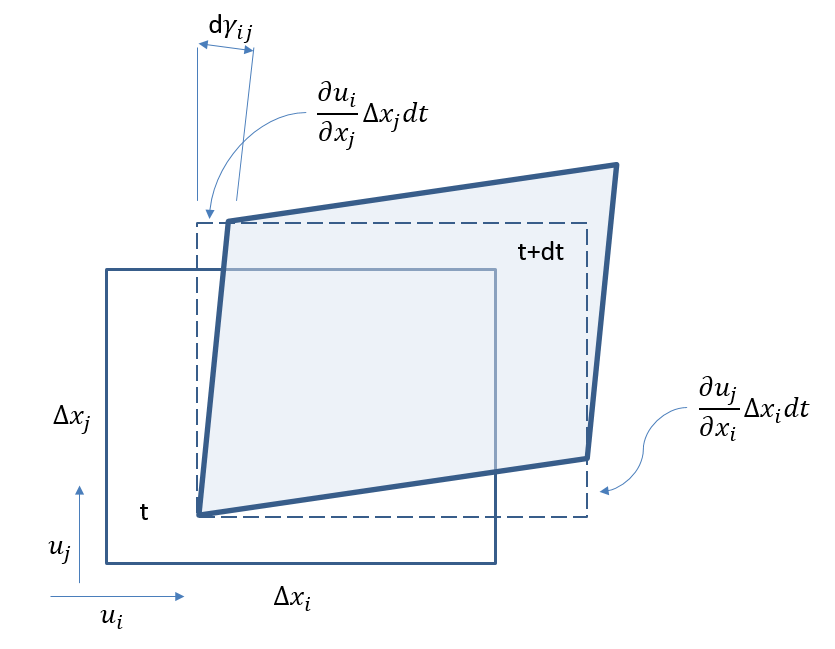
\includegraphics[width=0.65\linewidth]{Figures/2.Chapter/shear_ij}
	\caption{Shear deformation in a fluid volume.}
	\label{fig:shear_xy}
\end{figure}
%

In this interval the shear stress $\tau_{ij}$ produces in the fluid volume an incremental shear strain, $d\gamma_{ij}$, that can be written in a fixed reference frame as 

%
	\begin{equation} \label{eq:shear_strain_I}
		d\gamma_{ij}={\left( \frac{\partial u_i}{\partial x_i} \delta x_i dt \right)}/{\delta x_i}+{\left( \frac{\partial u_j}{\partial x_j} \delta x_j dt \right)}/{\delta x_j}
	\end{equation}
%
In a Lagrangian perspective, the rate of shear strain can be written as

%
	\begin{equation} \label{eq:shear_strain_II}
		\frac{d\gamma_{ij}}{dt}=\frac{\partial u_j}{\partial x_i}+ \frac{\partial u_i}{\partial x_j}
	\end{equation}
%
Imposing assumptions i) and ii), the shear stress is given by

%
	\begin{equation} \label{eq:newtonian_fluid_II}
		\ve{\tau} = \mu \frac{d\gamma_{ij}}{dt}=\mu \left( \frac{\partial u_i}{\partial x_j}+ \frac{\partial u_j}{\partial x_i} \right)=\mu (\ve{\nabla}\ve{u}+ (\ve{\nabla}\ve{u})^T)=2\mu\ve{D} ; \;\;\;\;\;\; (i \neq j)
	\end{equation}
%
where $\ve{D}$ is the strain rate tensor. Assumption iii) imposes that the coefficient of proportionality $\mu$, the shear viscosity coefficient, is the same for any direction and independent from any kinematic quantities. 

Expression \eqref{eq:newtonian_fluid_II} is valid in the case of incompressible flow, where Equation \eqref{eq:navier_cont} is reduced to $\nabla\cdot\ve{u}=0$ and isotropic stresses are not related to shear stresses. If the flow is compressible however, this relationship takes the form of

%%
%	\begin{equation} \label{eq:newtonian_fluid_III}
%		\ve{\tau} = -\left( p_t +\left(\frac{2}{3}\mu - \lambda \right)\ve{\nabla}\cdot\ve{u} \right)\delta_{ij} + \mu \left( \frac{\partial u_i}{\partial x_j}+ \frac{\partial u_j}{\partial x_i} \right)
%	\end{equation}
%%
%
	\begin{equation} \label{eq:newtonian_fluid_III}
		\ve{\tau} = \lambda \text{tr}( \ve{D})\ve{I} + 2\mu\ve{D}
	\end{equation}
%
%where $p_t$ represents the thermodynamic pressure, not the mechanical pressure $p$ and is written as $p_t=p+\lambda\ve{\nabla}\cdot\ve{u}$. The thermodynamic pressure is pressure that would exist if the fluid were in static equilibrium at the local density and temperature. 
where $\lambda$ is another proportionality coefficient, called bulk viscosity\footnote{For the sake of simplicity, the derivation of Equation \eqref{eq:newtonian_fluid_III} was not shown. The details can be consulted on \cite{Batchelor-2000} and \cite{Aris-1962}.}. The effect on the flow of the term which involves the bulk viscosity is usually very small even in compressible flows \citep{Batchelor-2000}. Only when density changes are induced either over extremely small distances (e.g. in the interior of shock waves, where they occur over a molecular scale) or over very short time scales (e.g. in high-intensity ultrasound) will the term involving $\text{tr}( \ve{D}) = \ve{\nabla}\cdot\ve{u}$ be large enough to have a noticeable effect \citep{Zeldovich-1967}.

Disregarding the terms introduced in Equation \eqref{eq:newtonian_fluid_III}, Equation \eqref{eq:ns_VIII} can finally be written as the Navier Stokes equation 

%
	\begin{equation} \label{eq:navier_momentum}
		\frac{d\ve{u}}{dt}= -\frac{1}{\rho}\ve{\nabla}p + \frac{1}{\rho}\mu \ve{\nabla}^2\ve{u} + \ve{g}
	\end{equation}
%




%%%%%%%%%%%%%%%%%%%%%%%%%%%%%%%%%%%%%%%%%%%%%%%%%%%%%%%%%%%%%%%%%%
\subsection{Boundary conditions}
\label{subsec:boundary_cond}


A particular flow problem may be solved by integrating the Navier-Stokes equation, together with the mass conservation equation plus whatever other equations are required to form a complete set, with the boundary conditions appropriate to the particular problem at hand. Equations \eqref{eq:navier_cont} and \eqref{eq:navier_momentum} are applied on a domain $\Omega$, bounded by $\partial\Omega$, composed of solid boundaries $\partial\Omega_B$ and free surfaces $\partial\Omega_F$. A solution yields the velocity components and pressure at the boundaries, from which one obtains the stress tensor via Equations \eqref{eq:cauchy_IV} and \eqref{eq:newtonian_fluid_II}.
In the absence of surface tension, the boundary conditions consistent with the continuum hypothesis are that i) the velocity components and ii) the stress tensor components must be continuous at all points in the domain, including across phase interfaces such as $\partial\Omega_B$ and $\partial\Omega_F$. These conditions can be translated into kinematic and dynamic impositions. The kinematic boundary condition reads

%
	\begin{equation} \label{eq:bc_kinematic}
		\ve{u}|_{\partial\Omega}=\overline{\ve{u}}|_{\partial\Omega},
	\end{equation}
%

where $\overline{\ve{u}}$ corresponds to an imposed velocity. This condition is inherently verified by the Lagrangian framework. The dynamic boundary condition must express ii), i.e., the continuity of stresses across the interface. Such condition is evident to impose at $\partial\Omega_B$

%
	\begin{equation} \label{eq:bc_ns_I}
		\ve{\sigma}|_{\partial\Omega_B}=\ve{\sigma}|_{\partial\Omega}; \;\;\;\;\forall: \partial\Omega_B \in \partial\Omega
	\end{equation}
%
Equation \eqref{eq:bc_ns_I} simply interprets \eqref{eq:cauchy_II} as a boundary condition. The same can be done in the case of the free-surface, typically imposing a given stress tensor, $\overline{\ve{\sigma}}$, at each point:

%
	\begin{equation} \label{eq:bc_ns_II}
		\ve{\sigma}|_{\partial\Omega_F}=(-p\ve{I}+ 2\mu\ve{D})|_{\partial\Omega_F}= \overline{\ve{\sigma}}|_{\partial\Omega_F}
	\end{equation}
%
After normal projections, one can write

%
	\begin{equation} \label{eq:bc_ns_III}
		p=2\mu \ve{n}\cdot\frac{\partial \ve{u}}{\partial\ve{n}}
	\end{equation}
%
where $\ve{n}$ is the unit vector normal to the free surface. This relation implies that the pressure field may be discontinuous at the free surface. 





\newpage
\section{Contact Mechanics for Fully Elastic Stiff Solids}
\label{sec:solid_model}

Contact mechanics considers geometrical and surface effects to deal with material bulk properties. The effects of geometrical effects on local elastic deformations seem to have been first considered by \cite{Hertz-1882}. The developed theory of Hertzian elastic deformation links the circular contact area of a sphere with a plane or another sphere with the elastic deformation of the materials. The original framework completely disregards any surface interactions. Adhesive interactions were introduced with the \ac{JKR} theory \citep{Johnson-1971}, using a balance between the stored elastic energy and the loss in surface energy, or interface energy. 

By analyzing the stresses at the contact of two elastic solids, small strains within the elastic limit can be assumed. The contact radius $a$ is considered significantly smaller than the radius of curvature $R_i$ of the two contacting surfaces, as depicted in Figure \ref{fig:sphere_contact}

%
\begin{figure}[ht!]
	\centering 
	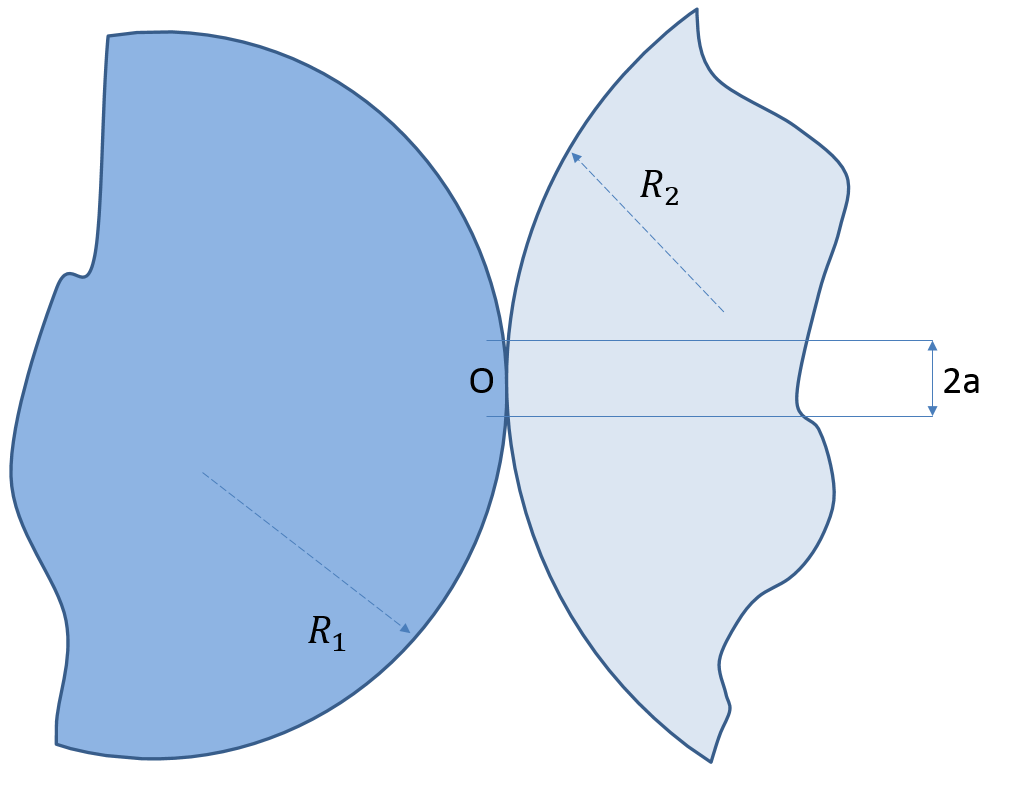
\includegraphics[width=0.55\linewidth]{Figures/2.Chapter/sphere_contact}
	\caption{Contact of two elastic spheres.}
	\label{fig:sphere_contact} 
\end{figure}
%
Assuming frictionless contact and using an elastic infinite half-space analysis, the contact radius $a$ can be written as

%
\begin{equation} \label{eq:hertz_I}
	a=\left( \frac{3FR^*}{4E^*} \right)^{\frac{1}{3}}
\end{equation}
%
where $F$ is the normal applied force, $R^*$ is the generalized radious of curvature of the interaction and $E^*$ is the generalized Young modulus, with

%
\begin{equation} \label{eq:hertz_II}
	R^*= \left( \frac{1}{R_1}+\frac{1}{R_2} \right)^{-1}; \;\;\;\; E^*= \left( \frac{1-\nu_{p1}^2}{E_1}+\frac{1-\nu_{p2}^2}{E_2} \right)^{-1}
\end{equation}
%
where $\nu_p$ is the Poisson ratio \citep{Johnson-1987}. The force is given by

%
\begin{equation} \label{eq:hertz_III}
	F=\frac{4}{3}E^*\sqrt{R^*}\delta^{3/2}
\end{equation}
%
where $\delta$ is the depth of indentation, a measure of the deformation of the sphere, given by $\delta=a^2/R^*$. The normal tension distribution (Hertz tension) can be estimated as

%
\begin{equation} \label{eq:hertz_IV}	
  p(r) = p_0\left(1-\frac{r^2}{a^2}\right)^{1/2};\;\;\;\;\;\   p_0 = \frac{3F}{2\pi a^2} = \frac{1}{\pi}\left(\frac{6F{E^*}^2}{{R^*}^2}\right)^{1/3} 
\end{equation}
%
where $r$ is the distance from the contact center.

The application of a tangential load $F_t$ to a Hertzian contact is done by assuming that normal stresses do not cause relative tangential displacements and shear stress do not produce relative normal displacements, i.e., in the absence of a tangential force, contacting points will not undergo tangential displacements \citep{Adams-2000}. It is usually assumed that, when $F_t$ is introduced, a central stick region surrounded by two slip zones is present. As the tangential force increases, the size of the stick region decreases and eventually sliding surfaces begins. This sliding respects Coulomb's friction law

%
\begin{equation} \label{eq:coulomb_friction}	
  F_t=\mu_f F_n 
\end{equation}
%
where $\mu_f$ is the friction coefficient. This law is general for static and kinetic friction, with a non-constant $\mu_f$ value. Conceptual models for the tensions developed prior to sliding are scarce. The traditional model is introduced in Chapter \ref{cap:chapter-numerical}, since it is described and assembled in discrete terms.


%\cleardoublepage
%% %%%%%%%%%%%%%%%%%%%%%%%%%%%%%%%%%%%%%%%%%%%%%%%%%%%%%%%%%%%%%%%%%%%%%%
% Dummy Chapter:
% %%%%%%%%%%%%%%%%%%%%%%%%%%%%%%%%%%%%%%%%%%%%%%%%%%%%%%%%%%%%%%%%%%%%%%

% %%%%%%%%%%%%%%%%%%%%%%%%%%%%%%%%%%%%%%%%%%%%%%%%%%%%%%%%%%%%%%%%%%%%%%
% The Introduction:
% %%%%%%%%%%%%%%%%%%%%%%%%%%%%%%%%%%%%%%%%%%%%%%%%%%%%%%%%%%%%%%%%%%%%%%
\fancychapter{Numerical Discretization}
\label{cap:chapter-numerical}

\textit{In this chapter the discretization methods are introduced and discussed, followed by a proposal for the discretization for the previously presented conceptual models. Competing formulations may be introduced in order to further justify a specific choice or drive a given idea. Continuous interpolation theory is explored, introducing interpolating kernels. Discrete interpolation is described and analyzed, with discrete differential operators being derived. The \ac{DEM} method is introduced and expanded within the \ac{SPH} framework. A time integration scheme is introduced and discussed briefly, as well as the corresponding stability region.}

\section{Integral Interpolation and the SPH Method}
\label{sec:SPH}

\subsection{Introduction}

In \ac{SPH} an approximate numerical solution is obtained by expressing the continuous media by a set of interpolation points from which to compute the quantities being conserved. These points represent material particles, since the Lagrangian description implies that they move with the flow, 'carrying' a given mass. This perspective into the fundamental idea of the method justifies the \emph{particle} term being applied, in the sense of a numerical mass lump, a macroscopic \emph{quanta} of the discretized medium. 

The method was introduced by \cite{Gingold-1977} and simultaneously by \cite{Lucy-1977}, initially to solve astrophysical problems where Eulerian mesh-based methods were insufficient. As a purely Lagrangian, meshless scheme, \ac{SPH} poses a number of advantages over mesh-based methods. Advection is treated explicitly, since particles carry their properties with them. Motion of the media maps directly as motion of the \ac{SPH} particles. This provides an important advantage for multi-phase problems, as each particle can be assigned to a different phase. Similarly, interfacial or free-surface flows do not require the explicit tracking of the interface or free-surface of interest, as it will be implicitly defined by the positions of the particles. Unlike mesh-based methods, there is no topological connectivity\footnote{Topological connectivity is employed in the context of a numerical discretization exclusively, meaning a fixed list of neighbors with whom to interact does not exist in \ac{SPH}.} between traditional \ac{SPH} particles, as they interact with all of the neighbors according to their radial separation, mediated by an interpolating kernel function. This has profound implications, as many of the issues with generation and evolution of a complex, time-varying mesh are bypassed. Problems involving complex, moving geometry, elastic solids or the fracture of brittle solids are significantly simpler to treat using Lagrangian meshless methods.

Disadvantages of the approach include mostly accuracy and stability concerns, due to their difficult formal description. \ac{SPH} particles are not constrained to stay in a well-ordered, stable configuration. In a regular lattice traditional techniques for stability analysis and convergence studies are well known; in a purely random sampling, as a Monte Carlo method, these qualities are also simple to compute, at least approximately. In \ac{SPH} however, any lattice deforms, not randomly, but according to the conservation equations being solved, introducing an unexpected difficulty in analyzing the method under normal conditions. If on one hand, by respecting the conservation equations, the particles tend to keep evenly spaced, the instantaneous dynamics of the medium can cause the particles to become locally disordered.  \cite{Monaghan-2005} presents an analysis of the interpolation errors that occur for a 1D equi-spaced line of \ac{SPH} particles. \cite{Swegle-1995} and \cite{Morris-1997} performed a stability analysis of \ac{SPH}, providing results for 1D and 2D regular grids of particles. In contrast, there is much less information available on \ac{SPH} errors and instabilities for disordered particles \citep{Ellero-2011}. \cite{Monaghan-2005} and \cite{Dehnen-2012} calculated an upper bound on the errors due to a randomly distributed set of particles, corresponding to a Monte Carlo simulation. Both noted that the distributions resulting from \ac{SPH} simulations are significantly more ordered than pure random positions, hence with higher accuracy than traditional Monte Carlo methods, as \cite{Quinlan-al-2006} explored by attempting to actually derive an error estimate for a generic SPH particle distribution. Even if second order seems to be the limit for traditional \ac{SPH} models \citep{Monaghan-2005, Oger-al-2007}, satisfactory results are achieved due to their inherent conservation properties, that coupled with the other advantages, seem to provide a uniquely useful tool.

%%%%%%%%%%%%%%%%%%%%%%%%%%%%%%%%%%%%%%%%%%%%%%%%%%%%%%%%%%%%%%%%%%%%%%%%%%%%%%%%%%%%%%%%%%
\subsection{Continuous Interpolation}
\label{Subsec:Interpolation}

Consider a scalar field A, expressed as a spatial convolution product with the Dirac Delta function $\delta$

%
\begin{equation} \label{eq:interpolant_1}
A\left( {\ve{r}} \right) = \int_\Omega  {A\left( {{\ve{r}}'} \right)\; \delta \left( {{\ve{r}} - {\ve{r}}'} \right)d{{r}}'},
\end{equation}
%
where $\Omega$ denotes the domain corresponding to the continuous medium. The nature of the Dirac Delta function renders \eqref{eq:interpolant_1} computationally inadequate, forcing its approximation by a suitable weight function $W\left( {{\ve{r}} - {\ve{r}}'} \right)$, called an interpolation kernel, which is a regular function and defines a compact support region\footnote{A function is said to have compact support if it is zero outside of a compact set. In the context of this work, the compact support region is therefore defined as the $\ve{r}$ centered region for which the kernel function $W$ is not zero.}. With $\Omega'$ being the domain centered in $\ve{r}$, one can write

% 
\begin{equation} \label{eq:interpolant_2}
A\left( {\ve{r}} \right) \approx  \left\langle {A} \right\rangle \left( {\ve{r}} \right) = \int_{\Omega '}  {A\left( {\ve{r}'} \right)\; W \left( {{\ve{r}} - {\ve{r}}'} \right)d{{r}}'},
\end{equation}
%
with $\left\langle {A} \right\rangle \left( {\ve{r}} \right)$ defining an interpolated field. Expanding field $A$ as a Taylor series around point $\ve{r}$ and writing $\bar{\ve{r}}=\ve{r}-\ve{r}'$

% 
\begin{equation} \label{eq:interpolant_taylor_1}
A\left( {\ve{r}'} \right) = A\left( {\ve{r}} \right) - \frac{\partial A}{\partial \ve{r}}\cdot \bar{\ve{r}} + \frac{1}{2}\bar{\ve{r}}^T \frac{\partial^2 A}{\partial \ve{r}^T \partial \ve{r}} \bar{\ve{r}} + O\left( |\bar{\ve{r}}|^3 \right)
\end{equation}
%
Replacing \eqref{eq:interpolant_taylor_1} back to \eqref{eq:interpolant_2}
% 
\begin{equation} \label{eq:interpolant_taylor_2}
\begin{split}
\left\langle {A} \right\rangle \left( {\ve{r}} \right) = A\left( {\ve{r}} \right) \int_{\Omega_0} {W \left( {\bar{\ve{r}}} \right)d{{r}}'} - \frac{\partial A}{\partial \ve{r}} \cdot \int_{\Omega_0} {\bar{\ve{r}} W \left( {\bar{\ve{r}}} \right)d{{r}}'} \; + \\ +\; \frac{1}{2} \text{tr}\left(\frac{\partial^2 A}{\partial \ve{r}^T \partial \ve{r}}\right) \cdot \int_{\Omega_0} {\bar{\ve{r}} \times \bar{\ve{r}} W \left( {\bar{\ve{r}}} \right)d{{r}}'} + \int_{\Omega_0} {O\left( |\bar{\ve{r}}|^3 \right) W \left( {\bar{\ve{r}}} \right)d{{r}}'}
\end{split}
\end{equation}
%
where $\Omega_0$ is $\Omega'$ translated to the origin. Noting that in such conditions $d{{r}'}=d\bar{{r}}$, for the approximation $\left\langle {A} \right\rangle \approx A$ to be accurate up to first order, then

% 
\begin{equation} \label{eq:kernel_cond_1}
\int_{\Omega_0} {W \left( \bar{{\ve{r}}} \right)d{{r}}'}=1
\end{equation}
%
and

% 
\begin{equation} \label{eq:kernel_cond_2}
\int_{\Omega_0} {W \left( \bar{{\ve{r}}} \right)\bar{\ve{r}}d{{r}}'}=0
\end{equation}
%

Condition \eqref{eq:kernel_cond_1} implies that the kernel zeroth-order moment should be equal to one, similarly to the Dirac delta distribution. Condition \eqref{eq:kernel_cond_2} asks that the kernel first order moment should be zero. By construction, $\Omega_0$ is centrally symmetric\footnote{A centrally symmetric object in Euclidean space is invariant under point reflection through its center.} and for an even kernel 

% 
\begin{equation} \label{eq:kernel_cond_3}
W \left( -\bar{{\ve{r}}}\right) =W \left( \bar{{\ve{r}}}\right)
\end{equation}
%
and
% 
\begin{equation} \label{eq:kernel_cond_4}
\nabla W \left( -\bar{{\ve{r}}}\right) =-\nabla W \left( \bar{{\ve{r}}}\right)
\end{equation}
%

Making a variable change $\bar{{\ve{r}}}'=-\bar{{\ve{r}}}$, one can write condition \eqref{eq:kernel_cond_2} as

% 
\begin{equation} \label{eq:kernel_cond_5}
\int_{\Omega_0} {W \left( \bar{{\ve{r}}} \right) \bar{\ve{r}} d\bar{\ve{r}}} = \int_{\Omega_0} {W \left( -\bar{{\ve{r}}} \right) \bar{\ve{r}} d\bar{\ve{r}}} = - \int_{\bar{\Omega}_0} {W \left( \bar{{\ve{r}}'} \right) \bar{\ve{r}'} d\bar{\ve{r}}'},
\end{equation}
%
where $\bar{\Omega}_0$ is the symmetric of $\Omega_0$. Assuming symmetrical invariance ($\bar{\Omega}_0 = \Omega_0$), the integral must be equal to its opposite, true only if both integrals are null, rendering condition \eqref{eq:kernel_cond_2} satisfied. We can now reduce \eqref{eq:interpolant_taylor_2} to 

% 
\begin{equation} \label{eq:interpolant_taylor_3}
\left\langle {A} \right\rangle \left( {\ve{r}} \right) = A\left( {\ve{r}} \right) \;+\; O(h^2),
\end{equation}
%
where the integral giving the error is $O(h^2)$ because $W \left( \bar{{\ve{r}}'} \right) \bar{\ve{r}'} d\bar{\ve{r}}' \sim 1/h$. 

Applying approximation \eqref{eq:interpolant_2} to the field $\nabla A$ we may write

% 
\begin{equation} \label{eq:grad_kernel_1}
\begin{split}
\left\langle {\nabla A} \right\rangle \left( {\ve{r}} \right) = \int_{\Omega '} \frac{\partial A \left( {\ve{r}'} \right)}{\partial {\ve{r}}'} \; W \left( \bar{\ve{r}} \right)d{\ve{r}}'\;= \\
=\; \int_{\Omega '} \frac{\partial}{\partial {\ve{r}}'} \left( A \left( {\ve{r}'} \right)\; W \left( \bar{\ve{r}} \right)\right)d{\ve{r}}'\; -\; \int_{\Omega '} A \left( {\ve{r}'} \right) \; \frac{\partial W \left( \bar{\ve{r}} \right)}{\partial {\ve{r}}'}d{\ve{r}}'
\end{split}
\end{equation}
%
It is important to write the identity 

% 
\begin{equation} \label{eq:grad_kernel_2}
\frac{\partial W \left( \bar{\ve{r}} \right)}{\partial {\ve{r}}'}= - \frac{\partial W \left( \bar{\ve{r}} \right)}{\partial {\ve{r}}}
\end{equation}
%
Applying the Gauss theorem to the first integral and the identity to the second yields

% 
\begin{equation} \label{eq:grad_kernel_3}
\left\langle {\nabla A} \right\rangle \left( {\ve{r}} \right) = \oint_{\partial\Omega '} A \left( {\ve{r}'} \right) \; W \left( \bar{\ve{r}} \right) \ve{n}\left( {\ve{r}'} \right) d\Gamma\;+ \; \int_{\Omega '} A \left( {\ve{r}'} \right) \; \frac{\partial W \left( \bar{\ve{r}} \right)}{\partial {\ve{r}}}d{\ve{r}}',
\end{equation}
%
where $\ve{n}\left( {\ve{r}'} \right)$ is the normal unit vector to $\partial\Omega'$. Assuming that the kernel has compact support, the surface integral is reduced to $\partial \Omega \cap \Omega'$ (refer to Figure \ref{fig:cont_kernel}). In an infinite domain, or with a sufficiently distant point $\ve{r}$ from $\partial \Omega$, this boundary integral is zero and Equation \eqref{eq:grad_kernel_3} renders

% 
\begin{equation} \label{eq:grad_kernel_4}
\left\langle {\nabla A} \right\rangle \left( {\ve{r}} \right) = \; \int_{\Omega '} A \left( {\ve{r}'} \right) \; \nabla { W \left( \bar{\ve{r}} \right)}d{\ve{r}}',
\end{equation}
%
This defines a continuously interpolated gradient operator, identical to \eqref{eq:interpolant_2}, but using the kernel gradient as the interpolation function. This is equivalent to writing

\begin{equation} \label{eq:grad_kernel_5}
\nabla \left\langle {A} \right\rangle \left( {\ve{r}} \right) = \left\langle {\nabla A} \right\rangle \left( {\ve{r}} \right) \;+\; O(h^2),
\end{equation}
%
demonstrated by applying the gradient operator to \eqref{eq:interpolant_taylor_3}. Inserting \eqref{eq:interpolant_taylor_1} into \eqref{eq:grad_kernel_4} we may write

% 
\begin{equation} \label{eq:grad_kernel_6}
\begin{split}
\left\langle {\nabla A} \right\rangle \left( {\ve{r}} \right) = \; A \left( {\ve{r}} \right)\int_{\Omega '} \nabla { W \left( \bar{\ve{r}} \right)}d{\ve{r}}' \; -\; \frac{\partial A}{\partial {\ve{r}}}\cdot \left( \int_{\Omega '} \nabla { W \left( \bar{\ve{r}} \right) \times \bar{\ve{r}} }d{\ve{r}}' \right) \;+ \\
+\; \frac{1}{2} \frac{\partial^2 A}{\partial \ve{r}^T \partial \ve{r}} \cdot\left( \int_{\Omega '} \nabla { W \left( \bar{\ve{r}}\right) \times \bar{\ve{r}} \times \bar{\ve{r}} }d{\ve{r}}' \right) \; + \; O(h^2)
\end{split}
\end{equation}
%
In order to have second-order accuracy on $\nabla \left\langle {A} \right\rangle \left( {\ve{r}} \right) \approx \left\langle {\nabla A} \right\rangle \left( {\ve{r}} \right)$ the conditions are

% 
\begin{equation} \label{eq:grad_kernel_cond_1}
\begin{split}
\int_{\Omega_0} \nabla { W \left( \bar{\ve{r}} \right)}d\bar{\ve{r}} \;=\: 0 \\
\int_{\Omega_0} \nabla { W \left( \bar{\ve{r}} \right) \times \bar{\ve{r}} }d\bar{\ve{r}} \;=\; -\ve{I} \\
\int_{\Omega_0} \nabla { W \left( \bar{\ve{r}}\right) \times \bar{\ve{r}} \times \bar{\ve{r}} }d\bar{\ve{r}} \;=\; 0
\end{split}
\end{equation}
%
where $\ve{I}$ is the identity. The first and last conditions are inherently satisfied by \eqref{eq:kernel_cond_4}. The second condition requires some manipulation:

% 
\begin{equation} \label{eq:grad_kernel_cond_2}
\begin{split}
\int_{\Omega_0} \nabla { W \left( \bar{\ve{r}} \right) \times \bar{\ve{r}} }d\bar{\ve{r}} = \int_{\Omega_0} \left[ \frac{\partial}{\partial \bar{\ve{r}}} \left( W \left( \bar{\ve{r}} \right)  \bar{\ve{r}} \right) - W \left( \bar{\ve{r}} \right) \left( \frac{\partial\bar{\ve{r}}}{\partial\bar{\ve{r}}} \right)^T  \right] d\bar{\ve{r}} \;=\\
=\; \oint_{\partial\Omega_0} W \left( \bar{\ve{r}} \right)\bar{\ve{r}} \times \ve{n}\left( \bar{\ve{r}} \right) d\Gamma\; -\; \left( \int_{\Omega_0} W \left( \bar{\ve{r}} \right) d\bar{\ve{r}}  \right)\ve{I}
\end{split}
\end{equation}
%
The surface integral is zero in the domain and property \eqref{eq:kernel_cond_1} renders the second condition of \eqref{eq:grad_kernel_cond_1} true.

A note should be made on a crucial assumption on these demonstrations, regarding a typical concern on interpolation methods: the boundaries. Conditions \eqref{eq:kernel_cond_1}, \eqref{eq:kernel_cond_2} and \eqref{eq:grad_kernel_cond_1} are true assuming that the compact support kernel $W \left( \bar{\ve{r}} \right) $ has no intersection with the boundary of the domain, \textit{i.e.} $\partial \Omega \cap \Omega' = 0$. Figure \ref{fig:cont_kernel} illustrates an intersection of $\partial \Omega $ and $\Omega'$.

%
\begin{figure}[ht!]
	\centering 
	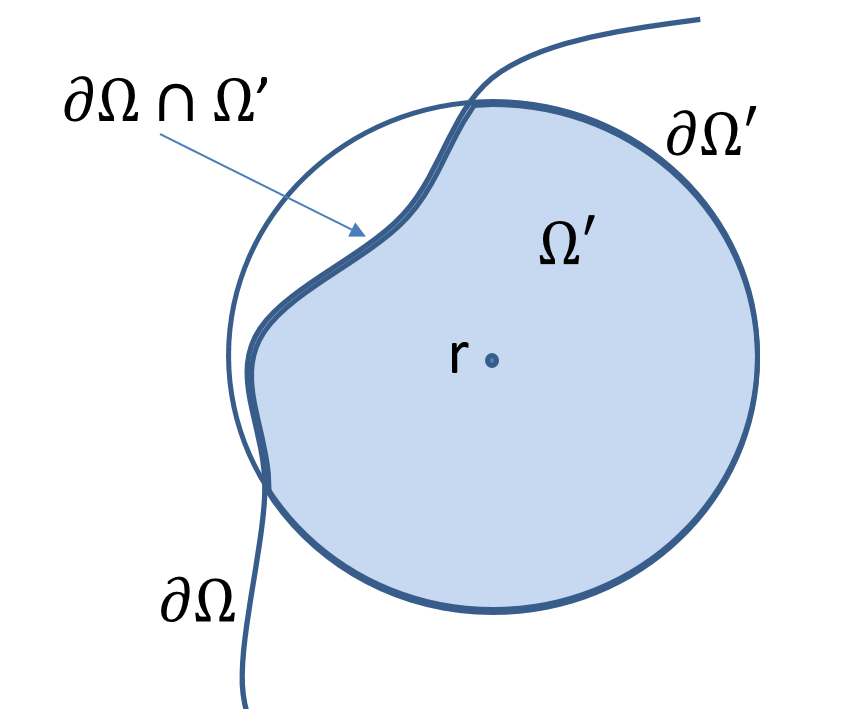
\includegraphics[width=0.30\linewidth]{Figures/3.Chapter/cont_kernel}
	\caption{Compact support kernel and domain boundary.}
	\label{fig:cont_kernel} 
\end{figure}
%
In this case the kernel zeroth-order momentum would not be one, deviating from the Dirac delta distribution and we would not be able to ensure first order consistency for the kernel approximation. Surface integrals in expressions \eqref{eq:grad_kernel_3} and \eqref{eq:grad_kernel_cond_2} would not disappear, leading to a loss of gradient information near the boundary and also order consistency. These problems meet various mitigation strategies at the discrete level, treated in section \ref{Subsec:discrete_interp}.

%%%%%%%%%%%%%%%%%%%%%%%%%%%%%%%%%%%%%%%%%%%%%%%%%%%%%%%%%%%%%%%%%%%%%%%%%%%%%%%%%
\subsection{Kernels}
\label{Subsec:Kernels}

In order to ensure the qualities of the continuous interpolation derived in Section \ref{Subsec:Interpolation}, the kernels must define a compact support region and have defined derivatives. A vast body of literature has been dedicated to the subject of kernels, their properties and their performance in the context of an \ac{SPH} simulation. Apparently similar kernels can produce very different results \citep{Monaghan-2005, Macia-2011,Violeau-2012}, and it is an ongoing task to formally identify and quantify the characteristics that lead to such differences. For the purpose of this thesis, only two kernels are described, a $5^{th}$ order class 2 Wendland \citep{Wendland-1995} and a cubic spline kernel. Both can be written as 

% 
\begin{equation} \label{eq:Kernel_general}
	W(\ve{r},h)=\frac{1}{h^d}\tilde{W}(q)
\end{equation}
%
where $h$ is the smoothing length and defines the scale of the compact support radius for kernel, $d$ is the dimensionality and $q=|\ve{r}|/h$ is a non-dimensional distance.

For the Wendland kernel, the $5^{th}$ order class 2 radial interpolation function was reformulated to have a $2h$ radius compact support

% 
\begin{equation} \label{eq:Kernel_wendeland}
	\tilde{W}(q)=\alpha_d\left\{ {\begin{array}{*{20}{c}}
  {(1-\frac{q}{2})^4(1+2q)} \\\\
  0 
\end{array}} \right.
\;\;\;\;\
\begin{array}{*{20}{c}}
  \text{for}\;\;\;{0 \leq q \leq 2} \\\\
  \text{for}\;\;\;{q > 2} 
\end{array}
\end{equation}
%
where $\alpha_d$ takes values $\alpha_2=7/4\pi$ and $\alpha_3=21/16\pi$. 

The cubic spline kernel can be defined as 

% 
\begin{equation} \label{eq:Kernel_cubic}
	\tilde{W}(q)=\alpha_d\left\{ {\begin{array}{*{20}{c}}
  {1-\frac{3}{2}q^2+\frac{3}{4}q^3} \\\\
  {\frac{1}{4}(2-q)^3} \\\\
  0 
\end{array}} \right.
\;\;\;\;\
\begin{array}{*{20}{c}}
  \text{for}\;\;\;{0 \leq q \leq 1} \\\\
  \text{for}\;\;\;{1 \leq q \leq 2} \\\\
  \text{for}\;\;\;{q > 2} 
\end{array}
\end{equation}
%
where $\alpha_2=10/7\pi$ and $\alpha_3=1/\pi$. Figure \ref{fig:kernel_wendland} plots the kernels and respective first derivatives.

%
\begin{figure}[ht!]
	\centering 
	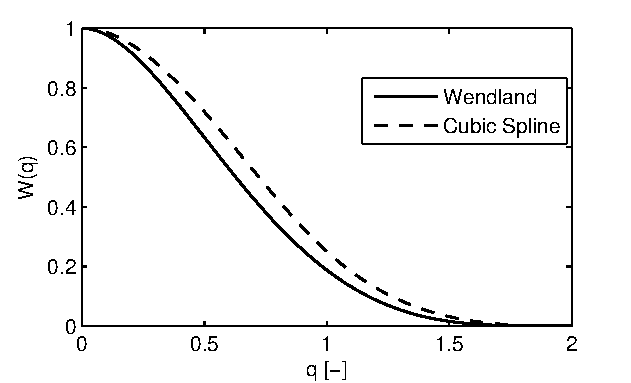
\includegraphics[width=0.49\linewidth]{Figures/3.Chapter/Kernels}
	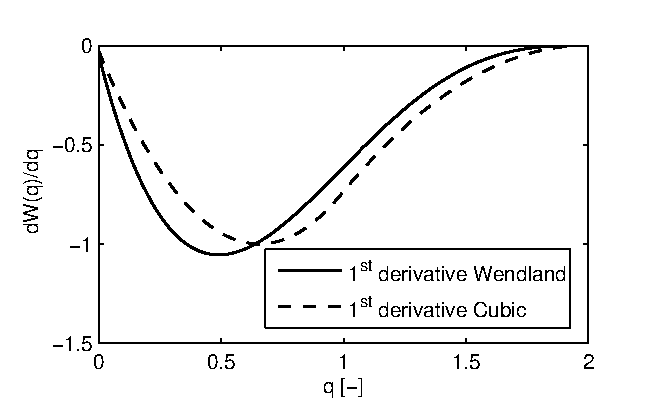
\includegraphics[width=0.49\linewidth]{Figures/3.Chapter/Kernels_deriv}
	\caption{Left - Wendland and Cubic spline kernels; Right - First derivatives.}
	\label{fig:kernel_wendland} 
\end{figure}
%
The kernels and the derivatives show very similar profiles, even tough they are one order apart. The cubic spline kernel is however known to cause tensile instability \cite{Monaghan-1999}, and requires corrections to definition \eqref{eq:Kernel_cubic}. According to \cite{Swegle-1995}, tensile instability seems to be directly related to the size of the region of the kernel where the second derivative is negative. Figure \ref{fig:kernel_wndland_d2} shows the second derivative of the considered kernels.

%
\begin{figure}[ht!]
	\centering 
	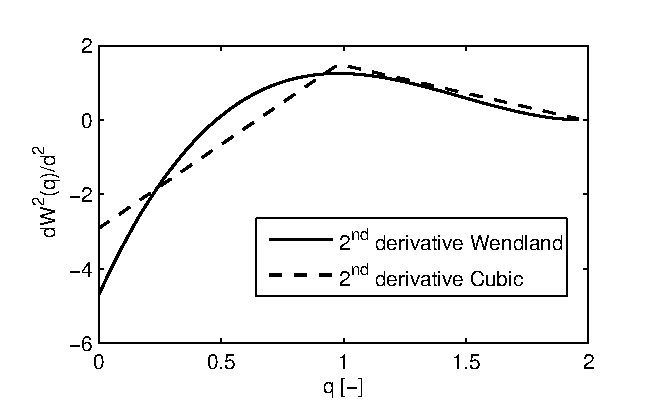
\includegraphics[width=0.49\linewidth]{Figures/3.Chapter/Kernels_2deriv}
	\caption{Second derivative of Wendland and Cubic spline kernels.}
	\label{fig:kernel_wndland_d2} 
\end{figure}
%
As can be noticed the size of these regions is similar, although the shape of the derivatives varies considerably. \cite{Macia-2011} performs an analysis of the performance of the Wendland kernel against a Gaussian kernel and finds that, even if apparently similar to the present comparison, the Wendland kernel out-performs other kernels considerably.


%%%%%%%%%%%%%%%%%%%%%%%%%%%%%%%%%%%%%%%%%%%%%%%%%%%%%%%%%%%%%%%%%%%%%%%%%%%%%%%%
\subsection{Discrete Interpolation}
\label{Subsec:discrete_interp}

As previously introduced, \ac{SPH} discretizes a continuous medium as a collection of Lagrangian interpolation nodes with mass. These points are called particles since they coincide with macroscopic material points that bear quantities such as velocity, density and position that change over time. Particle $i$ has a fixed mass of $m_i$, with volume $V_i$ and density $\rho_i$ related by

% 
\begin{equation} \label{eq:mass_volume_density}
V_i=\frac{m_i}{\rho_i}
\end{equation}
%
Assuming a reference density, a diameter $Dp$ can be set to compute the mass and reference volume of the particle.

In a strict Lagrangian framework, quantities of the particle will suffer a variation rate given by its Lagrangian derivative. For example, in the case of position and velocity

% 
\begin{equation} \label{eq:lagrang_posit}
\dot{\ve{r}}_i = \ve{v}_i = \frac{d\ve{r}_i}{dt}
\end{equation}
%
Expression \eqref{eq:lagrang_posit} contrasts with the Eulerian equivalent, since no advection terms are present, greatly simplifying the discretization.

The discretization of operators in \ac{SPH} is done by approximating the continuous integrals in section \ref{Subsec:Interpolation} by discrete summations. Employing a Riemann sum, one can write a scalar field as

% 
\begin{equation} \label{eq:discr_interp_1}
\left\langle {A} \right\rangle \left( {\ve{r}_i} \right) = \int_{\Omega '}  {A\left( {\ve{r}'} \right)\; W \left( {{\ve{r}_i} - {\ve{r}}', h} \right)d{{r}}'} \approx \sum_j{A_j V_j W(\ve{r}_{ij}, h)}
\end{equation}
%
The summation points are particle positions $\ve{r}_{j}$, where $A_j=A(\ve{r}_{j})$. $\ve{r}_{ij}$ represents $\ve{r}_{i}-\ve{r}_{j}$ and the volume of each $j$ particle accounts for the integration volume $d{\ve{r}}'$. Henceforth, without any loss of richness, the notation will be simplified: the subscripts $i$ and $j$ will tend to identify particles in the summation, $\ve{r}_{ij}$ will be used and it will be assumed that, dealing with a numerical approximation, the approximation notation will simply be represented by equality. The field is defined by the summation over all particles, but assuming compact support of the kernel this number is rendered finite. The sum is reduced to the particles inside the sphere of radius $\epsilon h$, as shown in Figure \ref{fig:kernel}

%
\begin{figure}[ht!]
	\centering 
	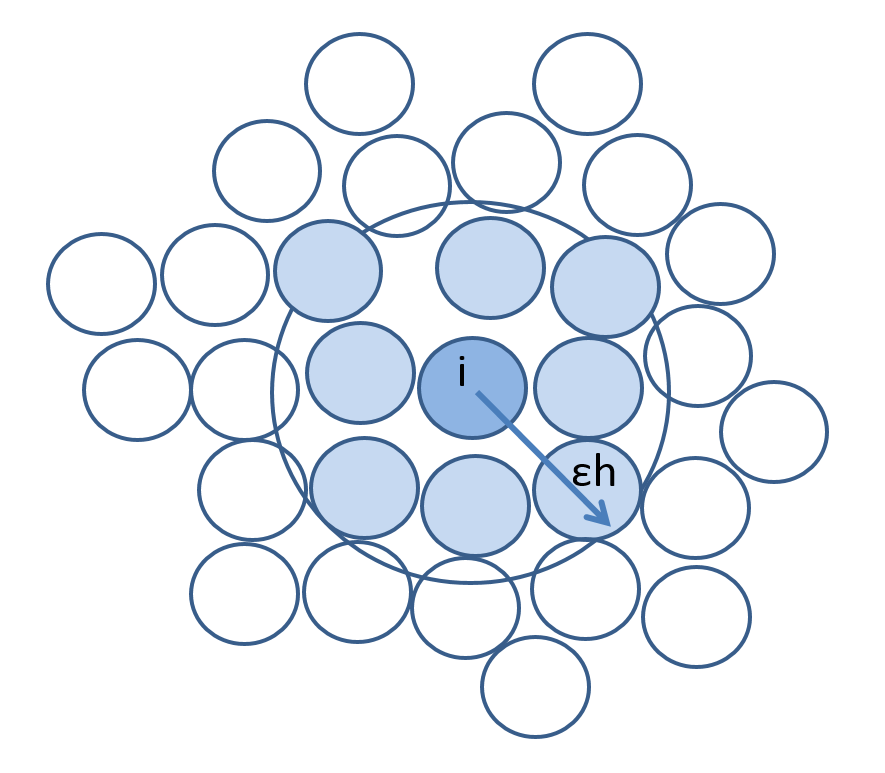
\includegraphics[width=0.40\linewidth]{Figures/3.Chapter/kernel}
	\caption{Summation extent for interpolation on particle $i$.}
	\label{fig:kernel} 
\end{figure}
%
In a 3 dimensions problem, the number of neighbors of a particle can range from a few tens to hundreds of points, summing an important disadvantage \ac{SPH} presents when compared with traditional, mesh-based methods: large computational cost.

Applying the discrete operator \eqref{eq:discr_interp_1} to vectorial quantities and notion \eqref{eq:grad_kernel_4} to differential operators we can write

% 
\begin{equation} \label{eq:discr_interp_2}
\begin{split}
A_i = \sum_j{A_j V_j W(\ve{r}_{ij}, h)} \\
\nabla {A}_i = \sum_j{A_j V_j \nabla W(\ve{r}_{ij}, h)} \\
\ve{A}_i = \sum_j{\ve{A}_j V_j W(\ve{r}_{ij}, h)} \\
\ve{\nabla} \cdot \ve{A}_i = \sum_j{ V_j \ve{A}_j \cdot \ve{\nabla} W(\ve{r}_{ij}, h)} 
\end{split}
\end{equation}
%

It should be noted that these expressions, although representing an exact derivative of the approximate function (considering no truncation effects on the kernel sampling), are written in a form that leads to a non zero derivative for a constant field. To ensure that gradients respect these properties one can write

% 
\begin{equation} \label{eq:discr_interp_3}
\nabla {A} = \frac{1}{\Phi}\left( \nabla(\Phi A)- A\nabla\Phi \right)
\end{equation}
%
where $\Phi$ is a differentiable function. In \ac{SPH} form

% 
\begin{equation} \label{eq:discr_interp_4}
\nabla {A}_i = \frac{1}{\Phi_i} \sum_j{\Phi_j V_j(A_j-A_i) \nabla W(\ve{r}_{ij}, h)}
\end{equation}
%
Equation \eqref{eq:discr_interp_4} returns a zero gradient for a constant field.  

Second derivatives can be estimated by differentiating an \ac{SPH} interpolant (Equation \eqref{eq:discr_interp_1}) twice:

% 
\begin{equation} \label{eq:2nd_der_sph_I}
\nabla^2 {A}_i  = \sum_j{A_j V_j \nabla^2 W(\ve{r}_{ij}, h)} 
\end{equation}
%
This expression, however elegant, presents a series of problems: i) it is very sensitive to particle disorder; ii) it is trivial to build a kernel whose second derivative changes sign on its defined region, possibly changing the sign of the second derivative independently of the behavior of the quantity, among other issues, properly explored by \cite{Brookshaw-1985, Monaghan-2005}. A more useful approach was proposed by \cite{Cleary-1996} and \cite{Morris-1997}

% 
\begin{equation} \label{eq:2nd_der_sph_II}
\nabla^2 {A}_i = \sum_j{A_j V_j \frac{\ve{r}_{ij}\cdot W(\ve{r}_{ij}, h)}{||\ve{r}_{ij}||^2}}
\end{equation}
%
This represents a hybrid combination of a finite difference derivative and a \ac{SPH} derivative. It has the advantage of bypassing the issues raised by taking a direct second derivative of the kernel function, at the expense of not fully conserving angular momentum \citep{Monaghan-2006}.


















\newpage
\section{Fluid discretization}
\label{sec:fluid-discretization}

This Section presents an attempt at discretizing Equations \eqref{eq:navier_cont} and \eqref{eq:navier_momentum}. With most particulate Lagrangian methods that is to say that the equations will be written with the corresponding discrete operators, in our case, the ones introduced in Section \ref{Subsec:discrete_interp}.

The continuity equation \eqref{eq:navier_cont} is traditionally discretized by employing the notion that $\rho \ve{\nabla} \cdot \ve{u} = \ve{\nabla} \cdot( \rho \ve{u}) - \ve{u} \cdot\ve{\nabla} \rho$, rendering equation \eqref{eq:navier_cont} as 
%
\begin{equation} \label{eq:sph_navier_cont}
	\frac{{d\rho_i }}{{dt}} = \sum_j{{m_j} \ve{u}_{ij} \cdot \ve{\nabla} W(\ve{r}_{ij}, h)}
\end{equation}
%
This is the equivalent of applying operator \eqref{eq:discr_interp_4} to approximate the $\ve{\nabla} \cdot \ve{u} $ field and taking $\Phi=\rho$. Equation \eqref{eq:sph_navier_cont} produces a zero divergence field for a constant $\ve{u}$ field. 

The approach of Sections \ref{Subsec:Interpolation} and \ref{Subsec:discrete_interp} was consistent with the designing of interpolation operators that would provide a desired accuracy. In particle methods, however, it becomes trivial and very tempting to interpret any equation in terms of pair-wise interaction between particles. For that purpose, we can agree that 

%
\begin{equation} \label{eq:physical_interp_I}
	\ve{\nabla} W(\ve{r}_{ij}, h) = \ve{r}_{ij}F(\ve{r}_{ij}, h)
\end{equation}
%
where $F(\ve{r}_{ij}, h) \leq 0$ is a function that respects Equation \eqref{eq:physical_interp_I}. The contribution of particle $j$ to the density variation of particle $i$ is then

%
\begin{equation} \label{eq:physical_interp_II}
	m_j\ve{u}_{ij} \cdot \ve{r}_{ij}F(\ve{r}_{ij}, h)
\end{equation}
%
This implies that approaching $ij$ particles i.e., for $\ve{u}_{ij} \cdot \ve{r}_{ij} \leq 0$, the interaction contributes with a positive density change, as our physical intuition expects. Equation \eqref{eq:sph_navier_cont} describes a medium that allows density changes, i.e., it is compressible. By allowing for \textit{some} compressibility the presented discretization is usually called \ac{WCSPH}. It has become the traditional \ac{SPH} way of modeling incompressible flows \citep{Monaghan-2005, Lee-2010}. Implementation is trivial since pressure is obtained from a \ac{EOS}, written so that the speed of sound is large enough to keep the relative density fluctuations small. \cite{Lee-2010} gives good insight into the relative accuracy of the pressure field of both \ac{WCSPH} and an incompressible approach, with the later being superior in most situations. Forcing incompressibility however, demands the solution of a large and potentially sparse Poisson problem at every time-step, built by defining a boundary at the free surface, that needs to be traced accurately. When dealing with highly distorted flows this is a major computational drawback and undermines the Lagrangian nature of the calculation. More details of the \ac{WCSPH} formulation are discussed in Section \ref{sec:eos}.

The pressure gradient of the Navier-Stokes equation (\eqref{eq:navier_momentum}) can be discretized in a number of ways. \cite{Gingold-1982} and \cite{Violeau-2012} used the discrete approximation of the Lagrangian of a particle system, using operators \eqref{eq:discr_interp_2} and \eqref{eq:discr_interp_4}. The same operators can be used directly to discretize the term in Equation \eqref{eq:navier_momentum}, leading to

%
 \begin{equation} \label{eq:sph_pressure_momentum}
\frac{\ve{\nabla}p_i}{\rho_i} = \sum_j{m_j \left( \frac{p_i}{\rho_i^2} +\frac{p_j}{\rho_j^2}\right) \ve{\nabla} W(\ve{r}_{ij}, h)},
\end{equation}
%
\noindent a symmetrical, balanced form of the pressure term that respects the action reaction principle. This implies that linear and angular momentum are conserved exactly by \eqref{eq:sph_pressure_momentum}. The second term of the second member in Equation \eqref{eq:navier_momentum} refers to the shear stresses, and it involves a second derivative of the velocity. As mentioned in Section \ref{Subsec:discrete_interp}, applying the SPH operators directly to the second derivative is avoided since it is too sensitive to particle disorder and limits the choice of the kernel functions. 

Three approaches to modeling this term are presented: the artificial viscosity model introduced by \cite{Gingold-1982}, the laminar viscosity model by introduced by \cite{Morris-1997} and the \ac{SPS} terms, properly presented in \cite{Dalrymple-2006} and discussed in Section \ref{sec:sps}.

\cite{Gingold-1982} introduced a momentum dissipating term in the form of a viscosity, designed to treat shock-tube problems. This form of numerical viscosity also mitigates problems due to instabilities arising in the system coming from the unstructured behavior of the particles, as well as accumulation of acoustic energy from integration errors during a simulation without dissipation. It is written as
%
\begin{equation}
\begin{split} 
\label{eq:sph_artificial_visc_I}
{
\ve{\Pi} _{i}} = \sum_j\left\{ {\begin{array}{*{20}{c}}
  {\frac{ \displaystyle { - \alpha {{\bar c}_{ij}}{\mu _{ij}}}}{\displaystyle {{{\bar \rho }_{ij}}}}\ve{\nabla}W(\ve{r}_{ij}, h)} \\ \\
  0 
\end{array}} \right.{\text{    }}\begin{array}{*{20}{c}}
  \text{if}\;\;\;{{{\ve{u}}_{ij}}\cdot{{\ve{r}}_{ij}} < 0} \\ \\
  \text{if}\;\;\;{{{\ve{u}}_{ij}}\cdot{{\ve{r}}_{ij}} \geqslant 0} 
\end{array} \;\;\; 
\hbox{with} \;\;\; {\mu _{ij}} = \frac{{({{\ve{u}}_{ij}}\cdot{{\ve{r}}_{ij}}}h)}{{{{r}}_{ij}^2}},
\end{split}
\end{equation}
%
\noindent where $c$ is the sound celerity and $\alpha$ is a parameter subject to calibration. This expression is traditionally used due to its simple implementation, conservation of linear and angular momentum and because it converges to $\mu {\ve{\nabla}^2}{\ve{u}}$ as $h \rightarrow 0$ \citep{Issa-2004}. It is however considered dissipative regarding shear and vorticity, and the case-dependent $\alpha$ parameter confirms its empirical nature.

\cite{Morris-1997}, influenced by the work of \cite{Cleary-1996}, proposed to model the shear viscosity by 

\begin{equation} \label{eq:sph_morris_laminar}
	\ve{\Pi}_{i} = \sum_j m_j \left( \frac{4\nu \ve{r_}{ij} \cdot \ve{\nabla}W(\ve{r}_{ij}, h) }{(\rho_i + \rho_j){{r}}_{ij}^2} \right)\ve{u}_{ij} 
\end{equation}
%
where $\nu$ is the actual kinematic viscosity of the fluid, defined as $\nu=\mu/\rho$. This expression conserves linear momentum but not angular momentum \citep{Colagrossi-2011}. Recent ideas over the local consistency of Expression \eqref{eq:sph_morris_laminar}, particularly in when the kernel is truncated, have been discussed by \cite{Colagrossi-2011} and \cite{Gonzalez-2009}.


The momentum equation (\eqref{eq:navier_momentum}) can now be written as
%\begin{equation} \label{eq:sph_navier_momentum}
%\begin{split}
%	\frac{{d{\boldsymbol{v}_i}}}{{dt}} = -\sum_j{m_j \left( \frac{p_i}{\rho_i^2} +\frac{p_j}{\rho_j^2} \right) \boldsymbol{\nabla} W(\boldsymbol{r}_{ij}, h)} +\\+ \sum_j m_j \left( \frac{4\mu \boldsymbol{r_{ij}} \boldsymbol{\nabla}W(\boldsymbol{r}_{ij}, h) }{(\rho_i + \rho_j)(|r_{ij}|^2 +\eta^2 )} \right)\boldsymbol{v}_{ij} + \sum_j{m_j \left( \frac{\tau_i}{\rho_i^2} +\frac{\tau_j}{\rho_j^2} \right) \boldsymbol{\nabla} W(\boldsymbol{r}_{ij}, h)} + {{\boldsymbol{g}}} 
%\end{split}
%\end{equation}
%%
\begin{equation} \label{eq:sph_navier_momentum_I}
	\frac{{d{\boldsymbol{u}_i}}}{{dt}} = -\sum_j{m_j \left( \frac{p_i}{\rho_i^2} +\frac{p_j}{\rho_j^2} \right) \boldsymbol{\nabla} W(\boldsymbol{r}_{ij}, h)} + \ve{\Pi}_{i} + \ve{g}
\end{equation}
%


%%%%%%%%%%%%%%%%%%%%%%%%%%%%%%%%%%%%%%%%%%%%%%%%%%%%%%%%%%%%
\subsection{Turbulence modeling}
\label{sec:sps}

Expressions \eqref{eq:sph_artificial_visc_I} and \eqref{eq:sph_morris_laminar} attempt to account for shear stresses developed at the scale of the interparticle interactions, $h$. Turbulent fluid flow however, may present very small local scales, depending on the Reynolds number, $R_e$ \citep{Batchelor-2000, pope-2000}. Attempting to model all of these scales is designated by \ac{DNS}, where no turbulent closures are needed. This imposes a serious limit on the range of possible $R_e$, since computational resources are limited. Opposite to this, the \ac{RANS} rely on closure models to estimate the stresses that arise even from large, energy-carrying structures. Another approach naturally compatible with our framework is to use \ac{LES} techniques, that can be understood as a intermediate between \ac{DNS} and \ac{RANS}. The idea is that the governing equations are spatially averaged over a length scale of the order of the numerical discretization. The contribution of the large structures to momentum and energy transfer is computed directly and only the effects of the smallest scales of turbulence are modeled. The hope is that, since the small scales tend to be more homogeneous and universal \citep{pope-2000}, the models can be simpler and require fewer adjustments when applied to different flows than similar models for the \ac{RANS}. 

To obtain the motion equations of the resolved scales, large and small scales must be separated. \ac{LES} is based on the definition of a filtering operation: a resolved variable is defined as

%
\begin{equation} \label{eq:eq_les_filter}
	\left\langle A \right\rangle(\ve{r})=\int_\Omega{A(\ve{r}')G\left( {{\ve{r}}, {\ve{r}}';\left\langle \Delta \right\rangle} \right)d{\ve{r}}'}  , 
\end{equation}
%
where $G$ is the filter function, the $\left\langle \; \right\rangle$ operator represents a generic spatial averaging and $\left\langle \Delta \right\rangle$ is the filter-width associated with the wavelength of the smallest scale retained by the filtering operation. Thus, the filter function determines the size and structure of the small scales. A special note should be given regarding the idea of the integral interpolant behind \ac{SPH} (Equation \eqref{eq:interpolant_1}) and the filtering operation of \ac{LES}. Since both \ac{SPH} and \ac{LES} share the same mathematical structure, it should come as no surprise that the combination of the methods seems very atractive to modelers.

\cite{Gotoh-2001} introduced this type of subgrid scaling for their incompressible \ac{MPS} method, as did \cite{Lo-2002} for their incompressible SPH method. For a compressible fluid, sub-particle scaling requires the use of special averaging, with Favre-averaging being the typically chosen in the literature. It is written as

%
\begin{equation} \label{eq:favre-average}
	\left\langle A \right\rangle=\frac{\left\langle\rho A\right\rangle}{\left\langle\rho\right\rangle}
\end{equation}
%
By using Favre-averaging, no new terms are introduced in the conservation equations, except for the \ac{SPS} terms. This means that Equations \eqref{eq:sph_navier_cont} and \eqref{eq:sph_navier_momentum_I} are implicitly in their filtered form, assuming $\left\langle A \right\rangle=A$\footnote{An acceptable abuse of notation since the averaged scale is indeed our working scale, no ambiguity is introduced.}. For the momentum Navier-Stokes equation, the application of a flat-top spatial filter yields \citep{Yoshizawa-1986} 

%
\begin{equation} \label{eq:navier_momentum_filtered}
		\frac{d\left\langle\ve{u}\right\rangle}{dt}= -\frac{1}{\left\langle\rho\right\rangle}\ve{\nabla}\left\langle p\right\rangle + \frac{1}{\left\langle\rho\right\rangle}\mu \ve{\nabla}^2\left\langle\ve{u}\right\rangle + \frac{1}{\left\langle\rho\right\rangle} \ve{\nabla}\cdot\ve{\tau}^* + \ve{g},
\end{equation}
%
where $\ve{\tau}^*$ is the \ac{SPS} tensor. Several proposals exist for the form of the tensor. Eddy-viscosity models try to reproduce the global exchange of energy between the resolved and unresolved stresses by mimicking the drain of energy associated with the turbulence energy cascade \citep{Batchelor-2000}. \cite{Yoshizawa-1986} proposed an eddy-viscosity model for weakly compressible turbulent flows using a multiscale direct-interaction approximation method. The anisotropic part of the \ac{SPS} is parametrized using the Smagorinsky (1963) model, while the \ac{SPS} energy is modeled by a  separate term

%
\begin{equation} \label{eq:sph_sps_visc}
	\frac{\ve{\tau}^*}{\left\langle\rho\right\rangle} = 2\nu_t \left( \left\langle\ve{D}\right\rangle - \frac{1}{3}\ve{\delta}\text{tr}\left(\left\langle\ve{D}\right\rangle\right) \right) - \frac{2}{3}C_I \Delta^2\ve{\delta}|\left\langle\ve{D}\right\rangle|^2,
\end{equation}
%
where $\nu_t=(C_S\Delta)^2|\left\langle\ve{D}\right\rangle|$ is the eddy viscosity, $C_S=0.1677$ is the Smagorinsky constant, $C_I=6.6\times10^{-3}$ and  $|\left\langle\ve{D}\right\rangle|=(2\left\langle\ve{D}\right\rangle\left\langle\ve{D}\right\rangle)^{1/2}$ \citep{Martin-al-2000}.

 
In \ac{SPH} notation, the \ac{SPS} term receives the same treatment as the pressure gradient term, in Equation \eqref{eq:sph_pressure_momentum}:

%
 \begin{equation} \label{eq:sph_sps_term}
\ve{\Pi}^{SPS}_{i} = \sum_j{m_j \left( \frac{\ve{\tau}^*_i}{\rho_i^2} +\frac{\ve{\tau}^*_j}{\rho_j^2}\right) \cdot \ve{\nabla} W(\ve{r}_{ij}, h)},
\end{equation}
%
where strain rate tensor is computed directly by approximating the velocity gradients with operator \eqref{eq:discr_interp_4} ($\Phi=\rho$). The $\Delta$ filter-width is typically taken as the distance between particles.


%%%%%%%%%%%%%%%%%%%%%%%%%%%%%%%%%%%%%%%%%%%%%%%%%%%%%%%%
\subsection{Density and pressure fields}
\label{sec:eos}

The \ac{WCSPH} formulation introduced by Equation \eqref{eq:sph_navier_cont} demands the usage of an \ac{EOS} to link the pressure and density fields. The most commonly employed \ac{EOS} is called Tait's Equation \citep{Batchelor-2000}, and is usually used to describe barotropic fluids:

%
\begin{equation} \label{eq:sph_state_equation}
	p_i = \frac{\rho_0 C_s^2}{\gamma} \left[ \left( \frac{\rho_i}{\rho_0} \right)^{\gamma} -1 \right]
\end{equation}
%
\noindent where $\rho_0$ is a reference density, $C_s$ is the numerical sound celerity and $\gamma=7$ for a fluid like water. It is used for free-surface flow because it assumes negligible atmospheric, or background, pressure.
$C_s=\sqrt{\partial p / \partial \rho}|_{\rho_0}$ \citep{Batchelor-2000} can be chosen large enough to render relative density fluctuations small, i.e., since

%
\begin{equation} \label{eq:sph_state_equation_cs}
	\frac{|\delta\rho_i|}{\rho_i} \sim \frac{u_i^2}{C_s^2}
\end{equation}
%
$C_s$ can be chosen as any percentage of the maximum velocity in the flow to ensure that the maximum density fluctuation is one order of magnitude lower. Typically $C_s$ is taken as $10\max u_i$, guaranteeing that $\max({|\delta\rho_i|}/{\rho_i}) \sim 0.01$. By using the first term of a Taylor expansion of Equation \eqref{eq:sph_state_equation_cs}, a linearized \ac{EOS} can be written as

%
\begin{equation} \label{eq:sph_state_equation_linear}
	p_i = {C_s^2}(\rho_i-\rho_0)
\end{equation}
%
This is built assuming locally smooth density gradients, and is usually used in the absence of a free-surface.

Equation \eqref{eq:sph_state_equation} represents a very stiff density field, and together with the natural disordering of the Lagrangian particles, high-frequency low amplitude oscillations are found to populate the density scalar field \citep{Molteni-2009}. The explored strategy in this work is to use a diffusive term in the continuity equation, now written as

%
\begin{equation} \label{eq:sph_navier_cont_delta_sph}
	\frac{{d\rho_i }}{{dt}} = \sum_j{{m_j} \ve{u}_{ij} \cdot \ve{\nabla} W(\ve{r}_{ij}, h)+\Phi_i}
\end{equation}
%
where

%
\begin{equation} \label{eq:delta_sph_molteni}
	\Phi_i =  2 \delta_\Phi h C_s \sum_j{(\rho_j-\rho_i) \frac{\ve{r}_{ij} \cdot \ve{\nabla} W(\ve{r}_{ij}, h)}{{r}_{ij}^2} \frac{m_j}{\rho_j}},
\end{equation}
%
This represents the original $\delta$-\ac{SPH} formulation by \cite{Molteni-2009}, due to the free parameter $\delta_\Phi$, that needs to be attributed a suitable value. It can be explained simply as the addition of the Laplacian of the density field to the continuity equation. \cite{Antuono-2012} has presented a careful analysis of the influence of this term in the system, by decomposing the Laplacian operator, observing the converge of the operators and performing linear stability analysis to inspect the influence of the $\delta_\Phi$ diffusive coefficient. Equation \eqref{eq:delta_sph_molteni} represents exactly a diffusive term in the domain bulk. The behavior changes close to open boundaries such as free-surface. Due to truncation of the kernel (there are no particles being sampled outside of an open boundary), the first order contributions of \eqref{eq:delta_sph_molteni} are not null \citep{Antuono-2010}, resulting in a net force applied to the particles. This effect is not considered relevant for non-hydrostatic situations, where this force is many orders of magnitude inferior to any other force involved. Corrections to this effect were proposed by \cite{Antuono-2010}, but involve the solution of a renormalization problem for the density gradient, with considerable computational cost.



%%%%%%%%%%%%%%%%%%%%%%%%%%%%%%%%%%%%%%%%%%%%%%%%%%%%%%%%
\subsection{Boundary Conditions}
\label{sec:BCs}

Boundary conditions must respect the ideas developed in Section \ref{subsec:boundary_cond}, particularly, that continuity of stresses across any interface must be respected. Another apparent advantage of particulate methods is that the condition is inherently satisfied since particles will respect Equations \eqref{eq:navier_cont} and \eqref{eq:navier_momentum} via their discrete forms, Equations \eqref{eq:sph_navier_cont} and \eqref{eq:sph_navier_momentum_I}. In \ac{SPH} however, the kernel is truncated near the boundaries and the imposition of a correct stress field at solid interfaces is demanding. The typical attempt at a solution is to complete the kernel on these regions, by introducing a series of boundary particles that may respect a different set of equations. Four major approaches are used for this effect: i)ghost particles, ii)repulsive particles, iii)dynamic particles and iv)boundary integrals. 

Ghost particles were initially devised by \cite{Randles-1996} in order to respect a no-slip condition at the same time that the kernel is not truncated. If a fluid particle is close to a solid boundary, for ($r_{ij}<h$), a new particle is generated as the specular image of the incident one, as the scheme in Figure \ref{fig:Ghost_particles}. 
%
\begin{figure}[H]
	\centering
	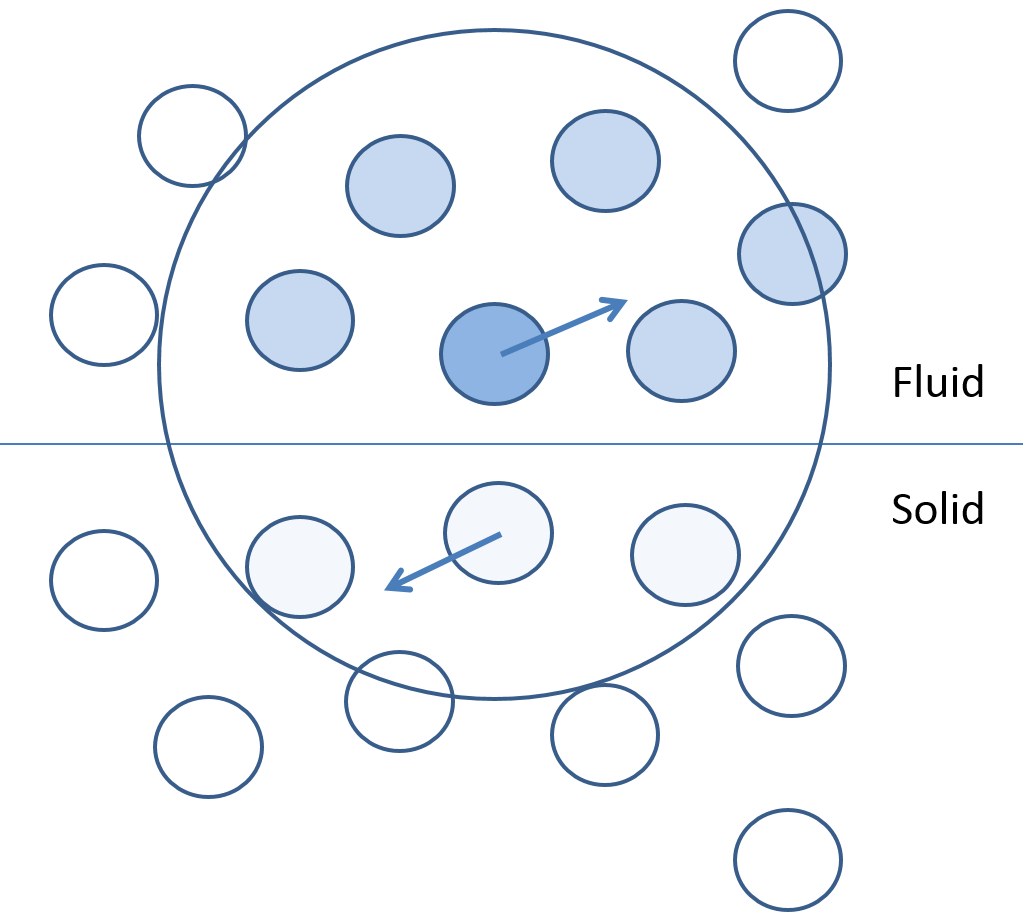
\includegraphics[width=0.45\linewidth]{Figures/3.Chapter/Ghost_particles}
	\caption{Scheme of ghost particles boundary condition.}
	\label{fig:Ghost_particles} 
\end{figure}
%

Both particles have the same density, but opposite normal and tangential velocities. Two disadvantages arise with this approach: complex geometries are extremely difficult to model (sharp angles, thin plates, hollow boxes) and the number of particles in the system may vary at each time step, a further implementation complication, explored in Section \ref{cap:chapter_hpc}. 


Repulsive particles \citep{Monaghan-1999} represent stationary particles that do not respect the conservation equations, but instead apply \textit{ad-hoc} forces to approaching fluid particles. The forces may be based on Lennard-Jones potentials, and a series of interpolation procedures are carried out to assure the continuity of a force field perceived by a fluid particle moving in an arbitrary direction from the boundary, as represented in Figure \ref{fig:repulsive_particles}.
%
\begin{figure}[H]
	\centering
	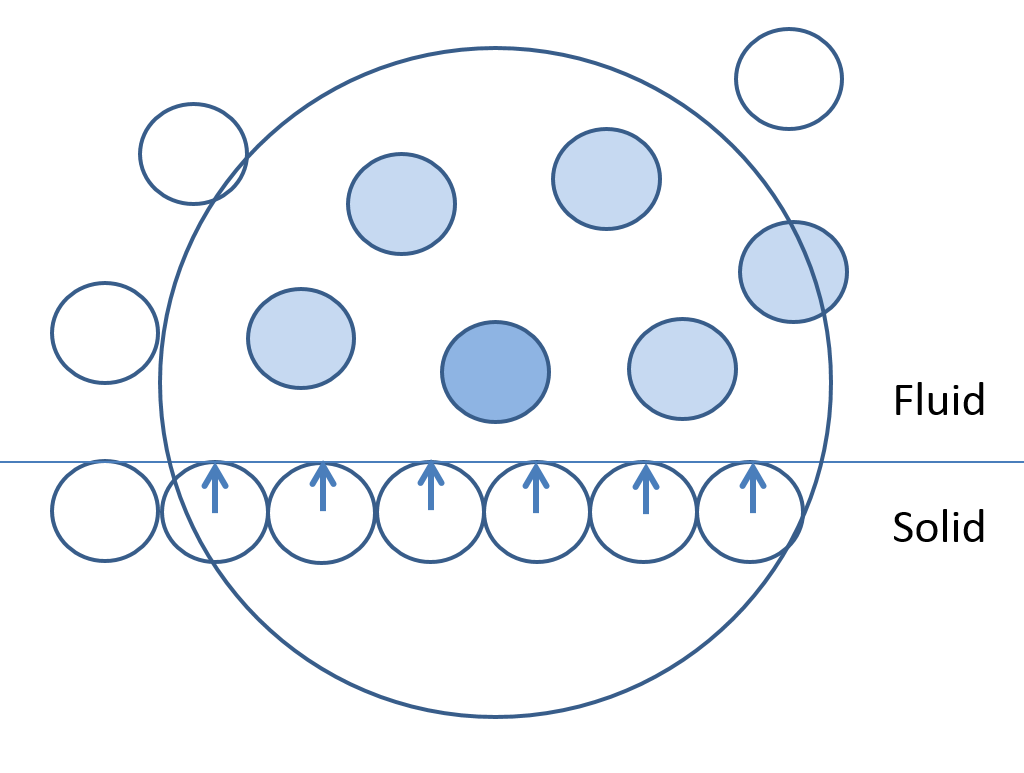
\includegraphics[width=0.45\linewidth]{Figures/3.Chapter/Repulsive_particles}
	\caption{Scheme of repulsive particles boundary condition.}
	\label{fig:repulsive_particles} 
\end{figure}
%

Dynamic particles were introduced by \cite{Dalrymple-2000} and further studied by \cite{Crespo-2007}, that devised them as fluid particles with an externally imposed motion. The particles respect Equations \eqref{eq:sph_navier_cont} and \eqref{eq:sph_navier_momentum_I} but their position is not given by integrating the velocity in time. A static boundary will have zero velocity (traditional arrangement in Figure \ref{fig:Dynamic_particles}) and a moving boundary will have a prescribed motion.
%
\begin{figure}[H]
	\centering
	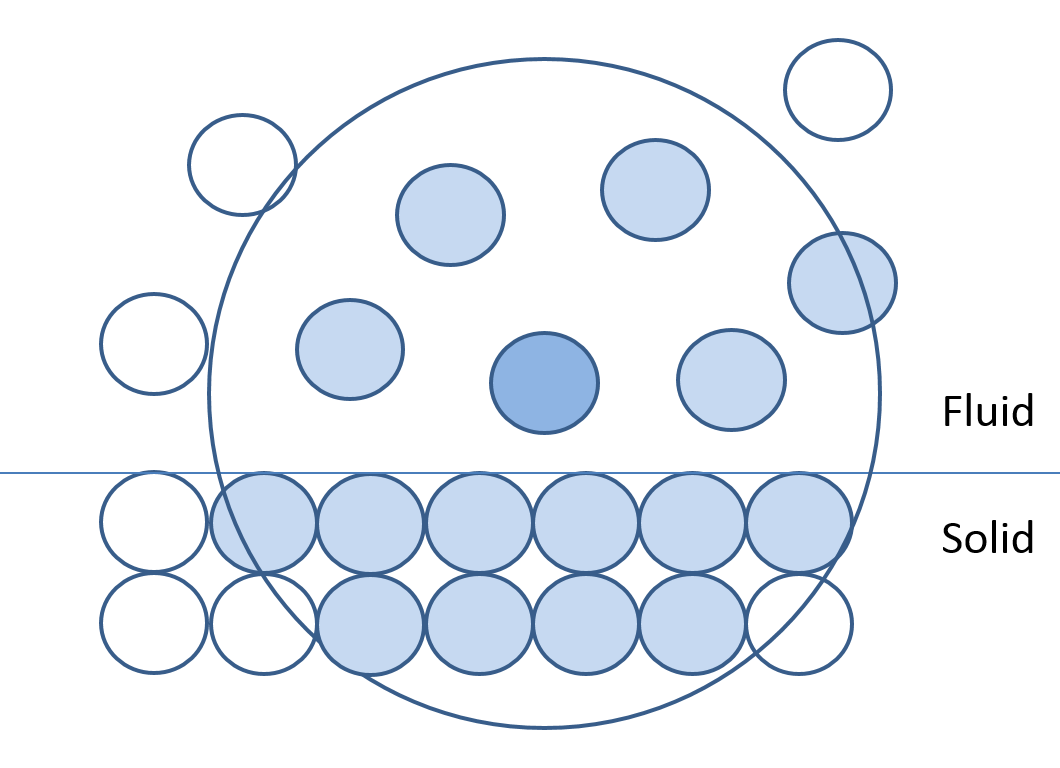
\includegraphics[width=0.45\linewidth]{Figures/3.Chapter/Dynamic_particles}
	\caption{Scheme of dynamic particles boundary condition.}
	\label{fig:Dynamic_particles} 
\end{figure}
%

A known difficulty of this formulation is the overestimation of the density \citep{Price-2008,Saitoh-2013}, resulting from an entropy jump across the fluid/solid interface. This results in an increased distance of fluid-solid particles due to the added force from the pressure gradient, effectively disturbing the viscous forces computed at that interface \citep{Colagrossi-2003}.

Boundary integral ideas are being explored in order to complete the kernel around boundaries, namely, analytically summing the missing terms. The boundary integral conditions \citep{Ferrand-al-2013, Mayrhofer-al-2015} are promising but still face many challenges related to complex geometries and efficient implementations.

This work will employ dynamic boundary conditions throughout, due to the simplicity and potential of the implementation. The solid body discretization presented in Section \ref{sec:solid-discretization} will also use the same framework.




\newpage
\section{Solid discretization: combining SPH and DEM}
\label{sec:solid-discretization}

The purpose of this Section is to devise a framework where the dynamics of solid bodies of arbitrary shape can be discretized in a way that solid-fluid interactions become trivial in the context of the fluid discretization presented in Section \ref{sec:fluid-discretization}. Section \ref{sec:solid-discretization_body} presents that general framework, where discrete equations for rigid body dynamics are introduced, generalizing the source of accelerations affecting a body. 

The \ac{DEM} model is introduced in Section \ref{sec:solid-discretization_force}, where the particular case of solid-solid interaction is explored. Traditional \ac{DEM} models are analyzed, as well as their numerical properties.

The result of this section is a \ac{DCDEM}, fully respecting the requirements of an accurate and robust model for the treatment of solid bodies with 6 \ac{DOF} in a multiphase setting.


\subsection{Rigid body discretization}
\label{sec:solid-discretization_body}

In the domain frame reference, the equations for a rigid body $I$ can be written as
%
\begin{equation} \label{eq:rigid_linear_newton}
	M_I\frac{d\ve{V}_I}{dt}=\sum_i \ve{F_i}
\end{equation}

\begin{equation} \label{eq:rigid_angular_newton}
	\ve{I}_I\frac{d\ve{\Omega}_I}{dt}=\sum_i(\ve{r}_i-\ve{R}_I)\times \ve{F_i},
\end{equation}
%
where body $I$ possesses a mass $M_I$, velocity $\boldsymbol{V}_I$, inertial tensor $\boldsymbol{I}_I$, angular velocity $\boldsymbol{\Omega}_I$ and center of gravity $\boldsymbol{R}_I$, and is subjected to an arbitrary number of forces $\ve{F_i}$, applied at points $\ve{r_i}$. 

In a particulate method it is trivial to idealize sub sets of particles in the domain whose variables are integrated in time with a different set of equations. If one uses Newton's equations for rigid body dynamics, then, that system of particles represents a rigid body. If body $I$ is a collection of particles\footnote{In this section $I$ is used for both the index of the rigid body in question and as the set of indexes from the particles that constitute the body. The abuse of notation is employed since in this context, they are semantically coincident.}, then the right side of Equations \eqref{eq:rigid_linear_newton} and \eqref{eq:rigid_angular_newton} can easily be discretized by

%
\begin{equation} \label{eq:rigid_linear}
	M_I\frac{d\ve{V}_I}{dt}=\sum_{k\in I} m_k \frac{{d{\ve{u}_k}}}{{dt}}
\end{equation}
%
\begin{equation} \label{eq:rigid_angular}
	\ve{I}_I\frac{d\ve{\Omega}_I}{dt}=\sum_{k\in I}m_k(\ve{r}_k-\ve{R}_I)\times \frac{{d{\ve{v}_k}}}{{dt}}
\end{equation}
%
$m_k {{d{\boldsymbol{u}_k}}}/{{dt}}$ represents the force by unit mass applied to particle $k$, belonging to body $I$. This force encompasses body forces (gravity), fluid resultants as well as the result of any rigid contact that might occur. This is inline with the work of \cite{Koshizuka-1998}, that first applied this idea in the context of \ac{MPS}.

Expressions \eqref{eq:rigid_linear} and \eqref{eq:rigid_angular} are obtained directly from applying \eqref{eq:rigid_linear_newton} and \eqref{eq:rigid_angular_newton} to a system of particles, i.e., they inherently conserve linear and angular momentum, as they are simple conservation laws. This is an advantage of particulate Lagrangian discretizations, since they are an exact representation of particle systems if the closure terms are also exact. For this system, it is simple to write the center of mass $\ve{R}_I$ and inertia tensor $\ve{I}_I$

%
\begin{equation} \label{eq:rigid_center_inertia}
	\ve{R}_I=\frac{1}{n_I}\sum_{k\in I} \ve{R}_k; \;\;\;\;\;\;\; \ve{I}_I=\sum_{k\in I}=m_k[\ve{r}_k-\ve{R}_I][\ve{r}_k-\ve{R}_I]
\end{equation}
%
where $n_I$ is them number of particles that constitute body $I$, $[\ve{r}_k-\ve{R}_I]$ is the skew-symmetric matrix built from $\ve{r}_k-\ve{R}_I$. Keeping in the domain frame reference implies that these quantities need to be recomputed whenever the system suffers an acceleration. 

Forces resulting from solid-fluid interaction are computed with Equation \eqref{eq:sph_navier_momentum_I}, where the viscous formulation provides a viscous drag closure. No \textit{ad-hoc} terms are added, since all the dynamics are a result of the fundamental, particle-wise, solution of Equations \eqref{eq:rigid_linear} and \eqref{eq:rigid_angular}.

This formulation can be seen as an extension of the dynamic boundary conditions introduced in Section \ref{sec:BCs}. As such, it suffers from the same overestimation of the density across the fluid/solid interface \cite{Price-2008,Saitoh-2013}, resulting from an entropy jump. The inclusion of the $\delta$-SPH diffusive term in Equation \eqref{eq:sph_navier_cont_delta_sph} allows for an apparently correct density estimation across the interface, as explored in the Results Section. The particles belonging to body $I$ are then moved according to

%
\begin{equation} \label{eq:rigid_propag_vel}
	\ve{u}_k= \ve{V}_I+\ve{\Omega}_I \times (\ve{r}_k-\ve{R}_I),
\end{equation}
%
\textit{i.e.}, the velocity given by propagating the rigid body velocities.


\subsection{Force discretization: the DEM model}
\label{sec:solid-discretization_force}

Forces $m_k {{d{\boldsymbol{u}_k}}}/{{dt}}$ will rise whenever a particle interacts with another. In the particular case of a solid-solid collision, the contact force is decomposed into $\ve{F}_n$ and $\ve{F}_t$, normal and tangential components respectively. Both of these forces will take forms explored in Section \ref{sec:solid_model}, with the addition of viscous dissipation effects. This is because two colliding bodies undergo a deformation which will be somewhere between perfectly inelastic and perfectly elastic, usually quantified by the normal restitution coefficient

%
\begin{equation} \label{eq:rest_coeff_def}
	e_n=-\frac{v_n|_{t=t^n}}{v_n|_{t=0}}, \;\;\;\; e\in[0,1]
\end{equation}
%
where $t=t^n$ is the instant at the end of collision and $t=0$ is the instant immediately before.

Forces are further decomposed into a repulsion force, $\boldsymbol{F}^r$, arising from the elastic deformation of the material, and a damping force, $\boldsymbol{F}^d$, for the viscous dissipation of energy during the deformation. Other dissipative mechanisms, such as plastic deformation and emission of elastic waves, excited from impact, will not be considered. The elastic waves are always present, but carry very little energy \citep{Shaefer-1996}, and are usually disregarded. Plastic deformation is not considered directly as its effects can, to some extent, be included in the viscous dissipation terms.

Figure \ref{fig:dem_scheme} generally illustrates the proposed viscoelastic DEM mechanism between two interacting particles.

%
\begin{figure}[ht!]
	\centering
	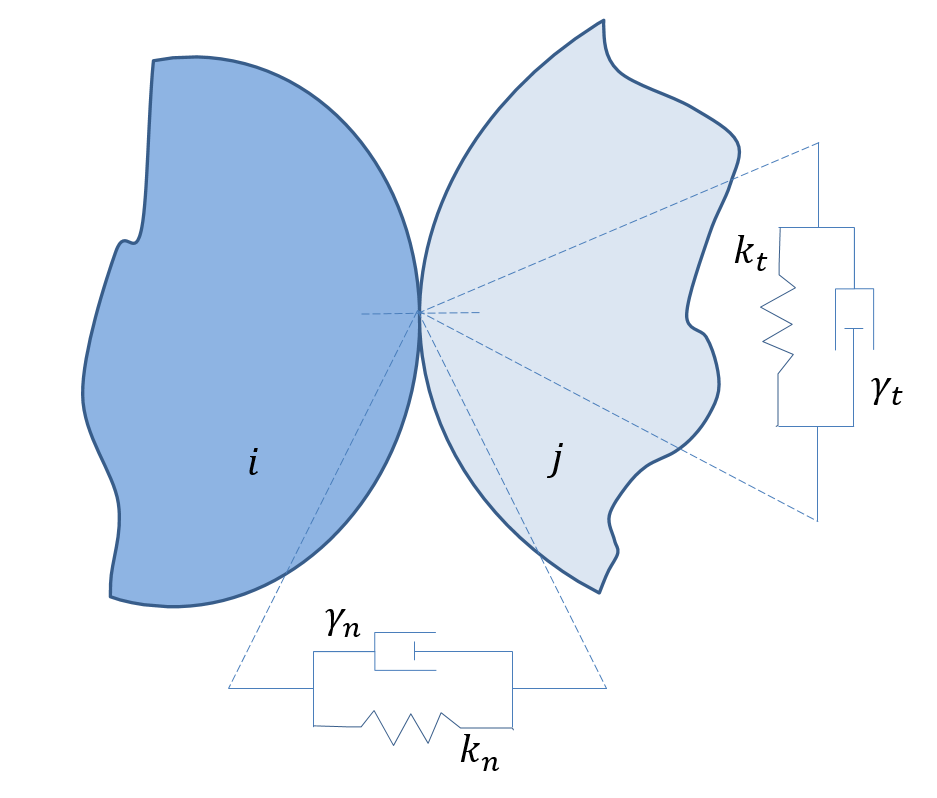
\includegraphics[width=0.60\linewidth]{Figures/3.Chapter/DEM_contacts}
	\caption{Scheme of DEM mechanism.}
	\label{fig:dem_scheme} 
\end{figure}
%
Every interaction is conceptualized as a system of springs and dampers. A general expression for the normal force in such viscoelastic model will be

%
\begin{equation} \label{eq:normal_viscoelastic_I}
	\ve{F}_{n,ij}=\ve{F}_n^r+\ve{F}_n^d=k_{n,ij}\delta_{ij}^{p_1}\ve{e}_{ij}-\gamma_{n,ij}\delta_{ij}^{p_2}\dot{\delta}_{ij}\ve{e}_{ij},
\end{equation}
%
where $k_{n,ij}$ is the normal stiffness constant of pair $ij$, $\delta_{ij}=\max(0, (d_i+d_j)/2-|\ve{r_{ij}}|)$ is the particle overlap, $\ve{e}_{ij}$ is the unit vector between the two mass centers and $\gamma_{n,ij}$ is the normal damping constant. For $p_1=p_2=1$, the mechanism is linear, corresponding to a simple damped harmonic resonator. An analytical solution \citep{Shaefer-1996} shows that this leads to a constant normal restitution coefficient, independent of the impact velocity

%
\begin{equation} \label{eq:linear_restitution_coeff}
	e_{n,ij}=\exp\left( -\frac{\gamma_{n,ij}}{2M^*}t_{c,ij} \right)
\end{equation}
%
where $M^*={m_im_j}/({m_i+m_j})$ and $t_{c,ij}$ is the contact duration, given by

%
\begin{equation} \label{eq:linear_tc}
	t_{c,ij}=\pi \left( \frac{k_{n,ij}}{M^*}- \left( \frac{\gamma_{n,ij}}{2M^*} \right)^2 \right)^{-1/2}
\end{equation}
%
Experimental studies using pendulum devices indicate that the $e_n$ and $t_c$ should depend on impact velocity however. Figures \ref{fig:Restitution_coeff} and \ref{fig:t_c_exp} both compiled by \cite{Kruggel-Emden-2007}, show that dramatic variations of these quantities may be registered.

%
\begin{figure}[ht!]
	\centering
	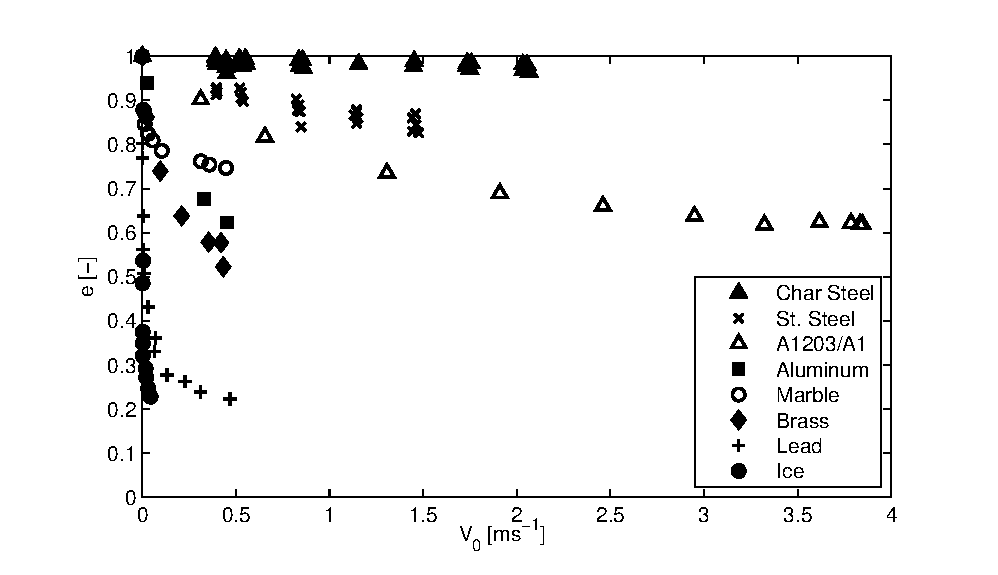
\includegraphics[width=0.73\linewidth]{Figures/3.Chapter/e_vo}
	\caption{Restitution coefficient $e$ as a function of initial normal velocity $V_0$ \citep{Kruggel-Emden-2007}.}
	\label{fig:Restitution_coeff} 
\end{figure}
%

%
%\begin{figure}[ht!]
%	\centering
%	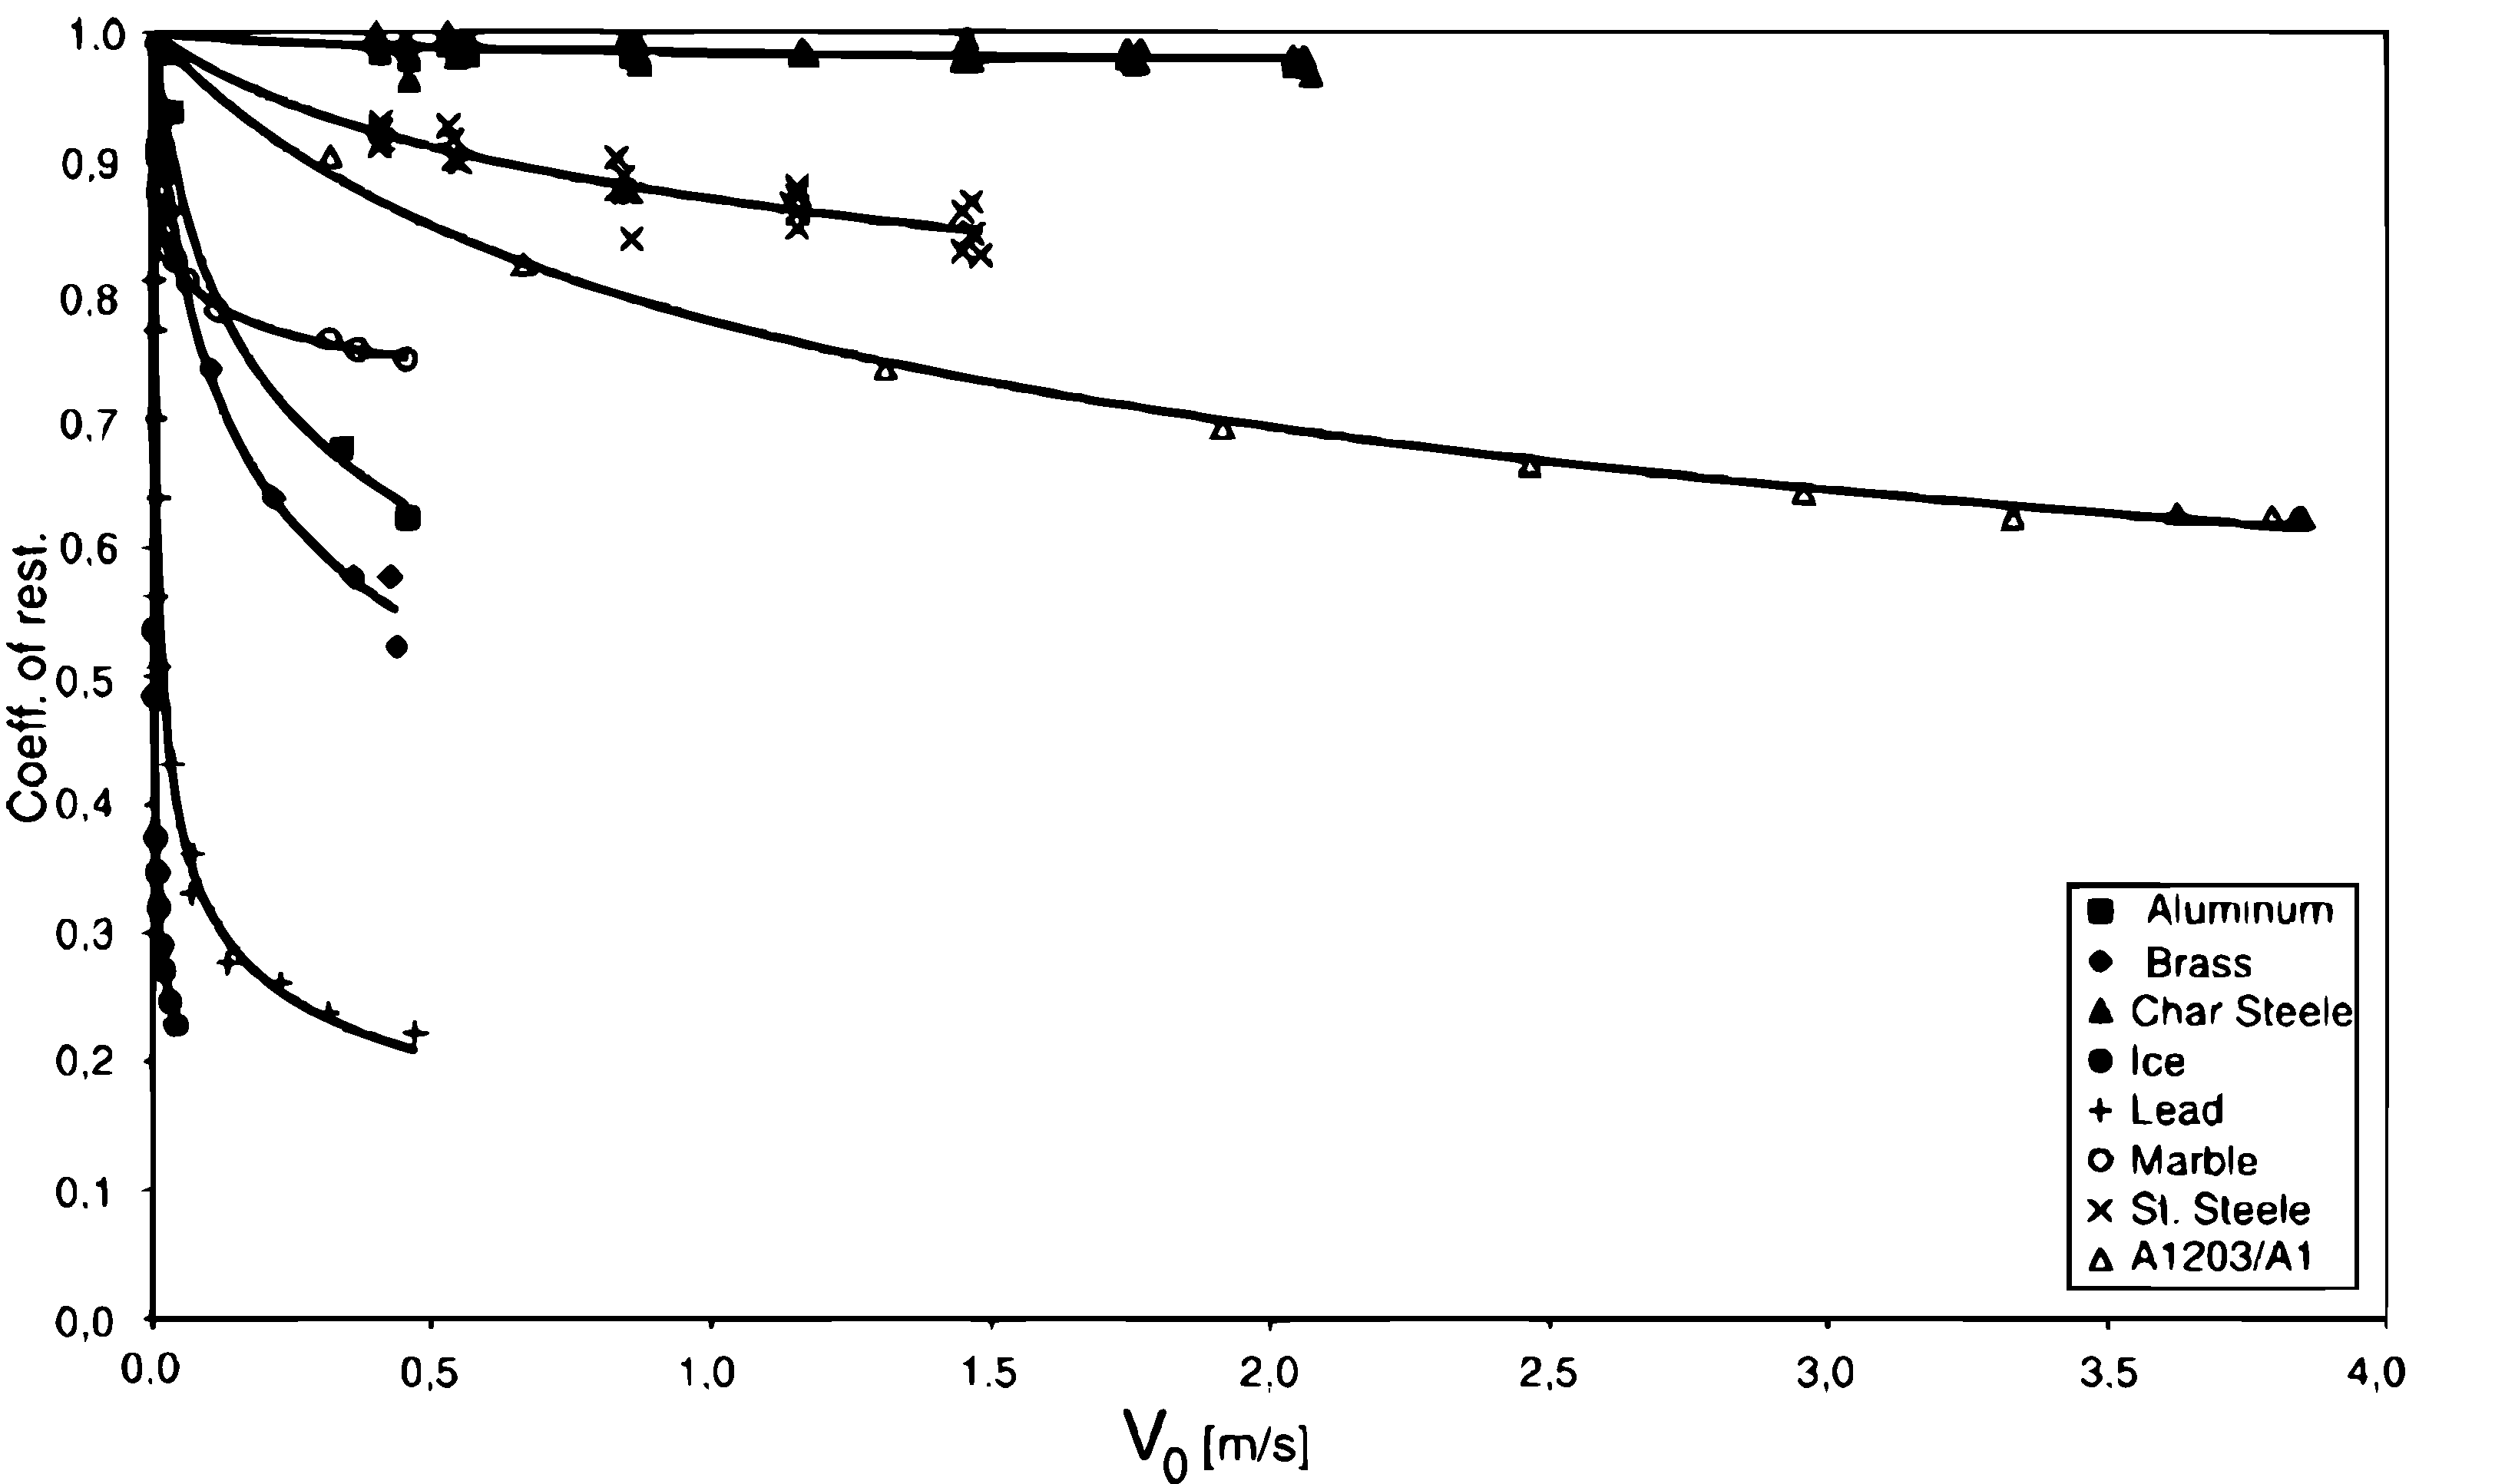
\includegraphics[width=0.80\linewidth]{Figures/3.Chapter/rest_coeff_exp}
%	\caption{Restitution coefficient $e$ as a function of impact normal velocity $V_0$ \citep{Kruggel-Emden-2007}.}
%	\label{fig:Restitution_coeff} 
%\end{figure}
%
%
\begin{figure}[ht!]
	\centering
	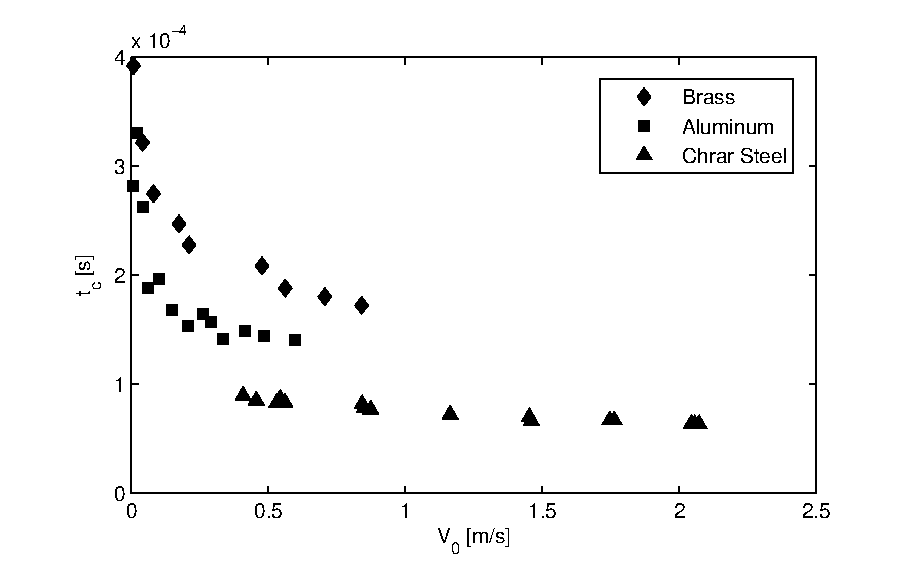
\includegraphics[width=0.70\linewidth]{Figures/3.Chapter/tc_vo}
	\caption{Duration of contact $t_c$ as a function of the impact normal velocity $V_0$ \citep{Kruggel-Emden-2007}.}
	\label{fig:t_c_exp} 
\end{figure}
%
%
%\begin{figure}[ht!]
%	\centering
%	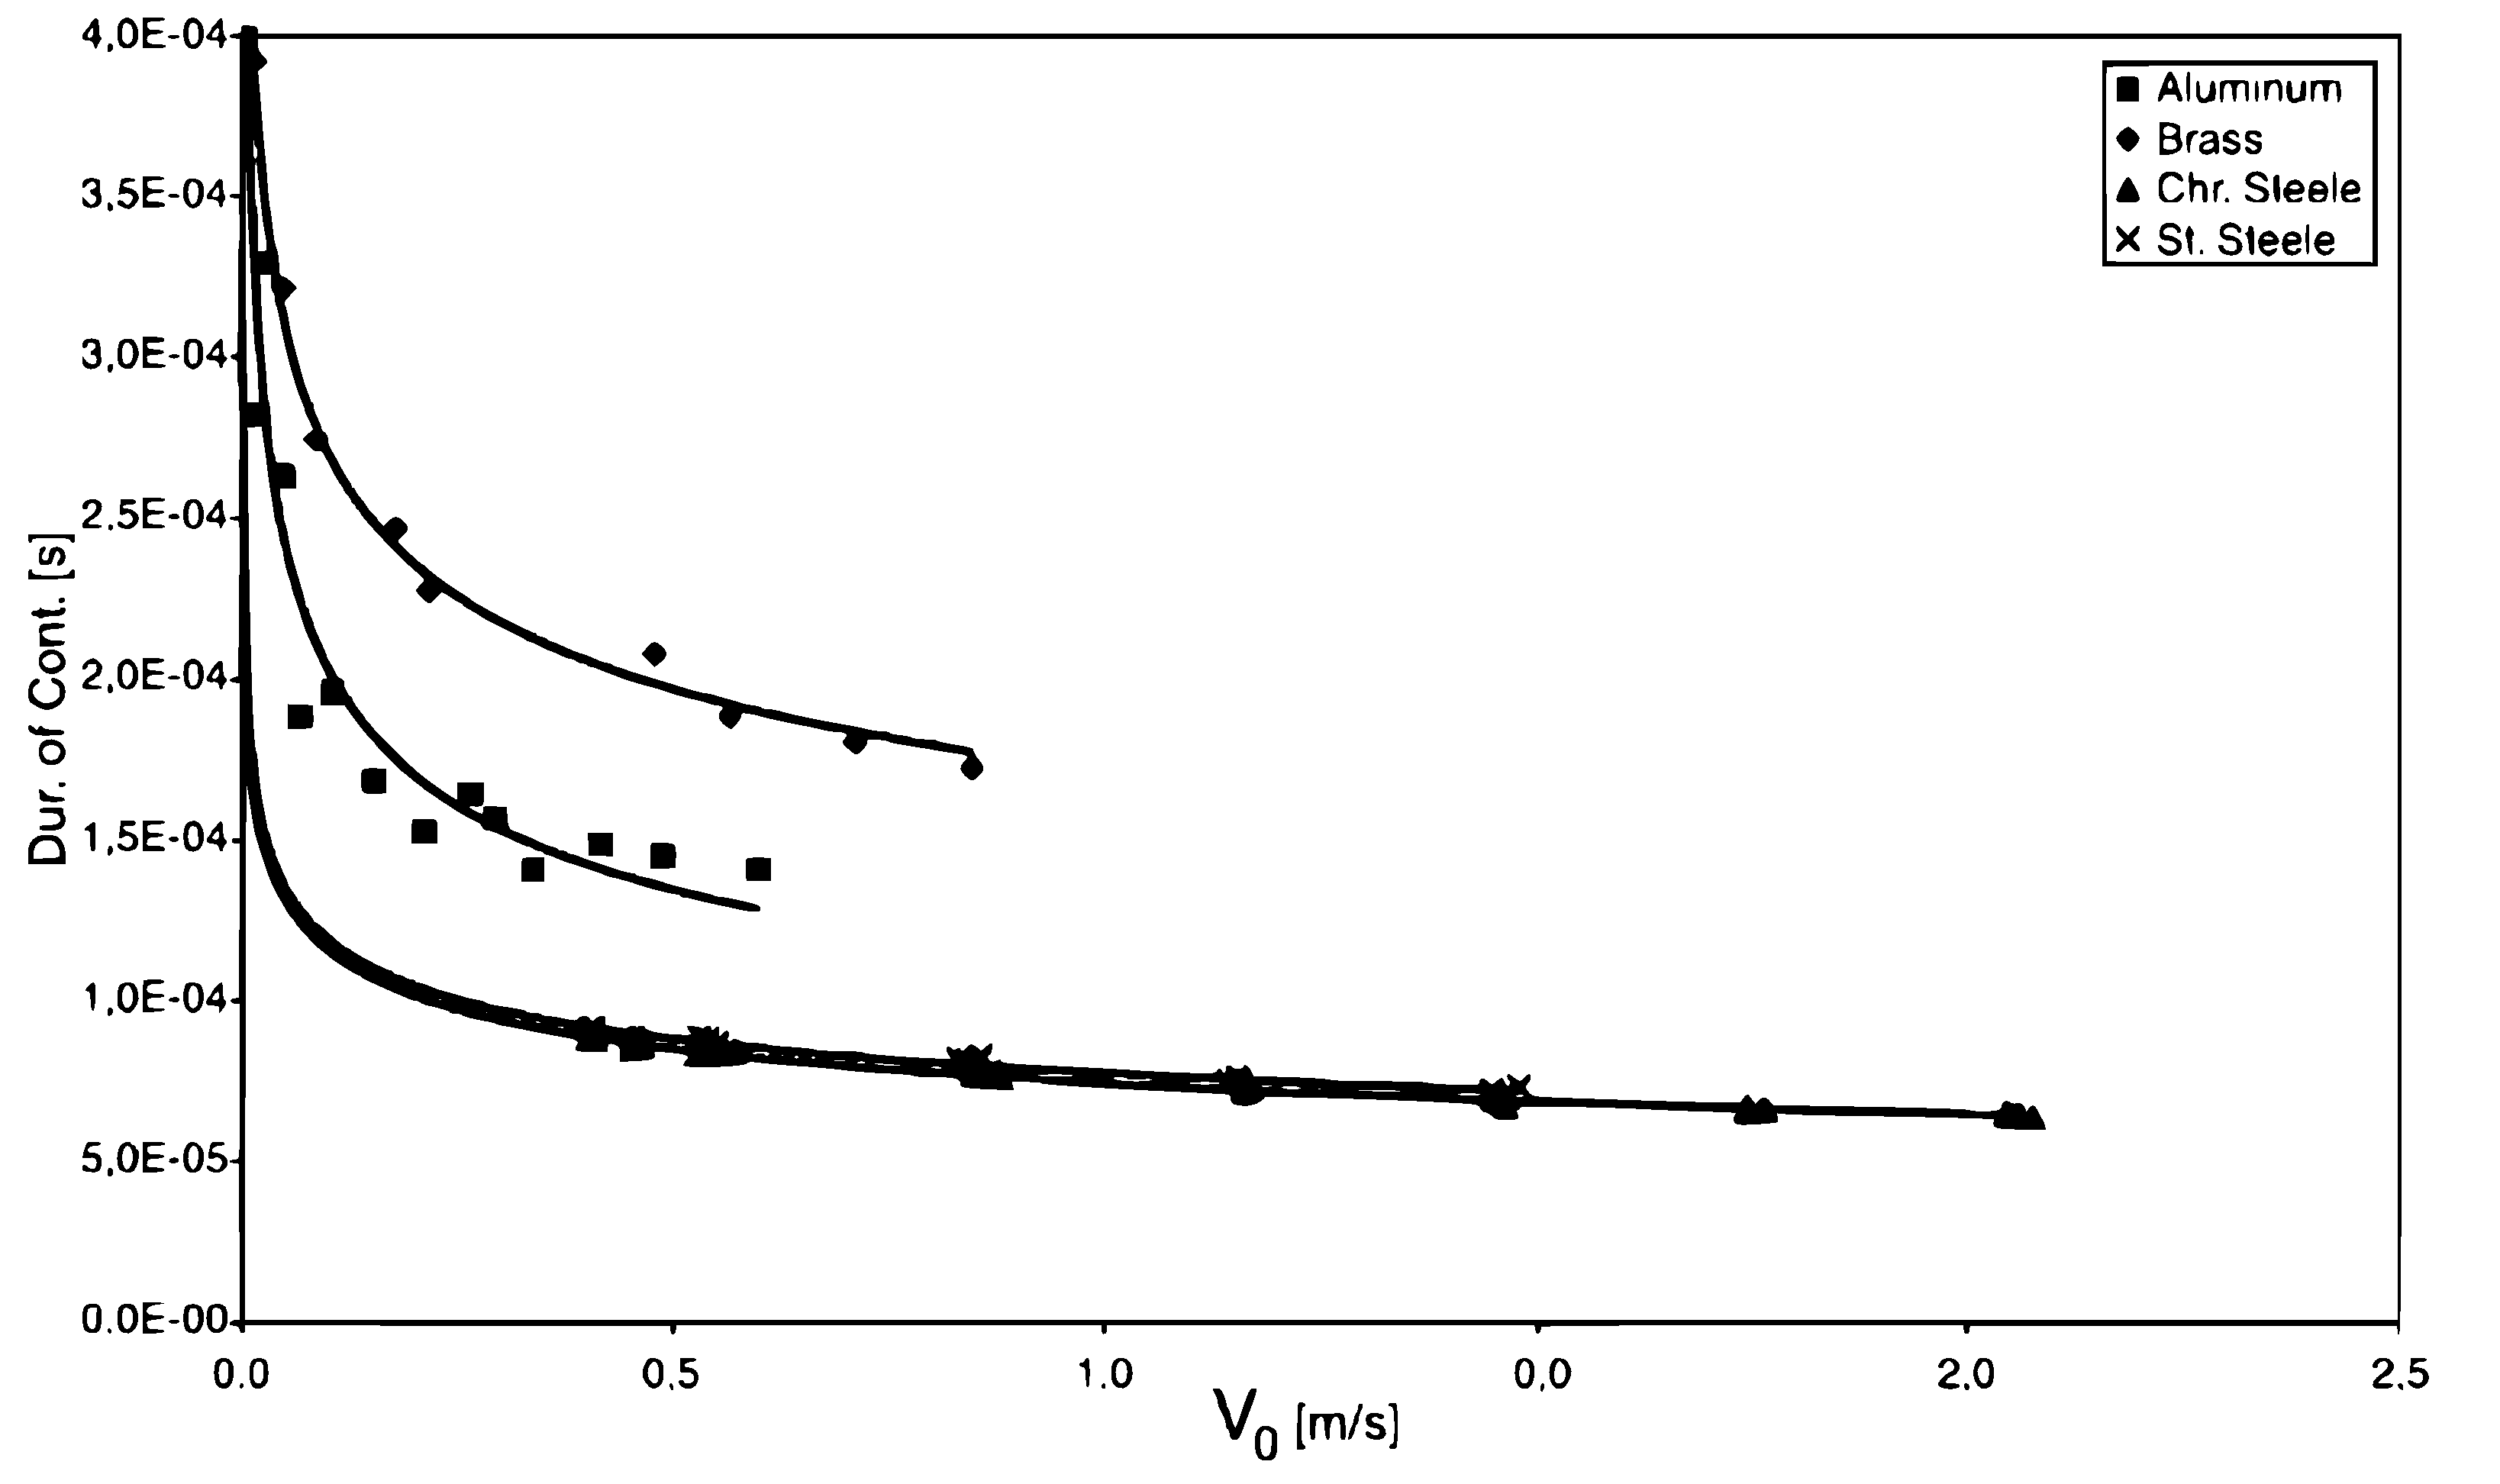
\includegraphics[width=0.80\linewidth]{Figures/3.Chapter/impact_time}
%	\caption{Duration of contact $t_c$ as a function of the impact normal velocity $V_0$ \citep{Kruggel-Emden-2007}.}
%	\label{fig:t_c_exp} 
%\end{figure}
%

Non-linear models allow to overcome the limitation imposed by a constant restitution coefficient and contact duration. \cite{Kuwabara-1987}, \cite{Brilliantov-1996} and \cite{Brilliantov-2001} proposed a fully non-linear model that reads

\begin{equation} \label{eq:non_linear_hertz_normal}
	\ve{F}_{n,ij}=\ve{F}_n^r+\ve{F}_n^d=k_{n,ij}\delta_{ij}^{3/2}\ve{e}_{ij}-\gamma_{n,ij}\delta_{ij}^{1/2}\dot{\delta}_{ij}\ve{e}_{ij},
\end{equation}
%
The stiffness, recovering the elastic Hertz model from Section \ref{sec:solid_model}, is given by a form of Equation \eqref{eq:hertz_III} 

%
\begin{equation} \label{eq:rigidity_hertz}
	k_{n,ij}=\frac{4}{3}E^*\sqrt{R^*}
\end{equation}
%
Considering exclusively the repulsive part of Equation \eqref{eq:non_linear_hertz_normal}, \cite{Shaefer-1996} notes that $t_{c,ij}$ is no longer independent from the normal velocity impact $v_{n,ij}$

%
\begin{equation} \label{eq:non_linear_tc}
	t_{c,ij}=3.21 \left( -\frac{M^*}{k_{n,ij}} \right)^{2/5}v_{n,ij}^{-1/5}
\end{equation}
%
implying that there is no longer an intrinsic time scale to collisions, as expected from experimental data.

\cite{Brilliantov-1996} and \cite{Brilliantov-2001} proposed that the viscous damper coefficient $\gamma_{n,ij}$ is a material property, obtainable from the bulk viscosities of the materials in collision and the local curvature at impact point. However, very little studies have been devoted to bulk viscosities and as a consequence $\gamma_{n,ij}$ is traditionally treated as a calibration parameter. \cite{Cummins-2011} writes an expression for $\gamma_{n,ij}$ depending exclusively on a normal restitution coefficient

%
\begin{equation} \label{eq:gamma_dem}
	\gamma_{n,ij}=-\frac{\log{e_{n,ij}}}{\sqrt{\pi^2+\log^2{e_{n,ij}}}}
\end{equation}
%
Expression \eqref{eq:gamma_dem} used in the context of a non-linear model, is ambiguous. In practice, a constant value for $e_{n,ij}$ will be used to compute $\gamma_{n,ij}$, that will lead to a non-constant, effective $e_{n,ij}$, depending on the impact velocity.

Figure \ref{fig:e_hertz} shows $e_{n,ij}$ as a function of $v_{n,ij}$, for the linear model and for the non-linear Hertz model (Expression \eqref{eq:non_linear_hertz_normal})

%
\begin{figure}[ht!]
	\centering
	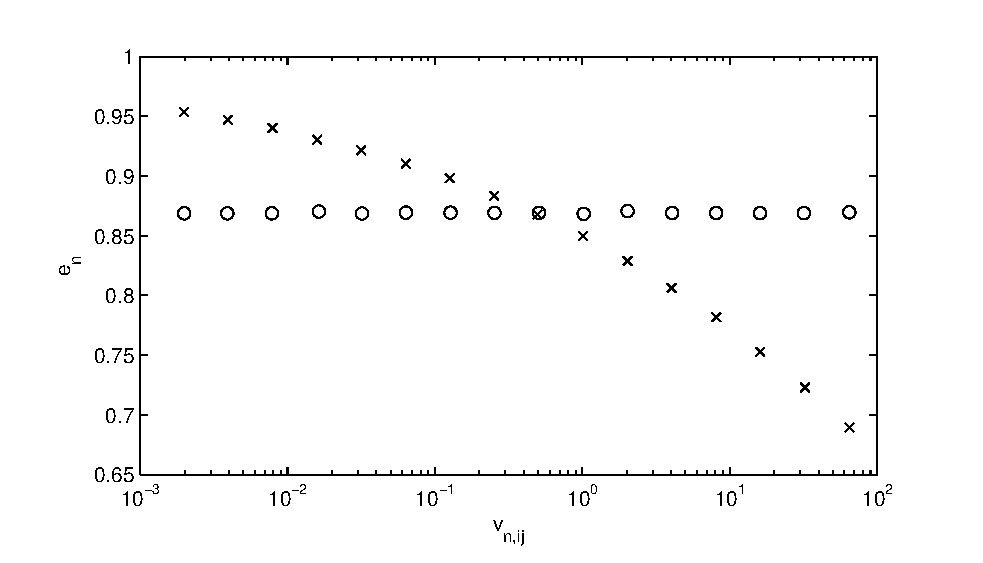
\includegraphics[width=0.80\linewidth]{Figures/3.Chapter/e_hertz}
	\caption{Normal restitution coefficient $e_{n,ij}$ as a function of the impact normal velocity $v_{n,ij}$. Linear force ($\circ$), Non-linear Hertz ($\times$)}
	\label{fig:e_hertz} 
\end{figure}
%
For the linear case $k_n=7.32\times10^6$ Nm$^{-1}$ and $\gamma_n=2.06$ kg s$^{-1}$, resulting in $e_n=0.87$. For the non-linear model, $\gamma_n=190$ m$^{-1/2}$s$^{-1}$, in order to produce comparable $e_n$ in the selected $v_{n,ij}$ range. As expected, the linear model produces a constant $e_n$. Force \eqref{eq:non_linear_hertz_normal} leads to an inversely proportional $e_{n,ij}$ with $v_{n,ij}$, i.e., $(1-e_{n,ij})\sim v_{n,ij}^{1/5}$, in agreement with experimental results (Figure \ref{fig:Restitution_coeff}).


Regarding tangential contacts, friction is modeled using the same model, as indicated in Figure \ref{fig:dem_scheme}. The mechanism can be reproduced by a linear dash-pot 

%
\begin{equation} \label{eq:elastic_fric}
	\ve{F}_{t,ij}=\ve{F}_t^r+\ve{F}_t^d=k_{t,ij}\delta^t_{ij}\ve{e}^t_{ij}-\gamma_{t,ij}\dot{\delta}^t_{ij}\ve{e}^t_{ij}
\end{equation}
%
where the stiffness and damping constants are derived to be

%
\begin{equation} \label{eq:fric_coeffs}
	k_{t,ij}=2/7k_{n,ij}; \;\;\;\;\; \gamma_{t,ij}=2/7\gamma_{n,ij},
\end{equation}
%
as to insure internal consistency of the time scales required for stability \citep{Hoomans-2000}. This mechanism models the static and dynamic friction mechanisms by a penalty method. The body does not statically stick at the point of contact, but is constrained by the spring-damper system. This force must be bounded above by the Coulomb friction law introduced by Equation \eqref{eq:coulomb_friction}. The Coulomb law is modified with a sigmoidal function in order to make it continuous around the origin regarding the tangential velocity \citep{Vetsch-2011}:

%
\begin{equation} \label{eq:fric_I}
	\ve{F}_{t,ij}=\min(\mu_{fIJ} \ve{F}_{n,ij} \tanh (8\dot{\delta}^t_{ij})\ve{e}^t_{ij};\;\; \ve{F}_{t,ij}),
\end{equation}
%
\noindent where $\mu_{fIJ}$ is the friction coefficient at the contact of $I$ and $J$ and is simply taken as the average of the two friction coefficients of the distinct materials.
\section{Time Integration and Stability Region}
\label{sec:dt}

The ordinary differential equations described in Sections \ref{sec:fluid-discretization} and \ref{sec:solid-discretization} may be integrated in time using a stable method. Traditionally Symplectic schemes are preferred in Hamiltonian systems due to the time-reversibility in the absence of dissipative terms, as well as implicit conservation properties \citep{Monaghan-2005}, leading to a lesser energy drift in long computations. Both \ac{SPH} and \ac{DEM} methods use the Symplectic scheme due to these characteristics. An explicit second-order with time accuracy of $O(dt^2)$ Symplectic integrator is used, using two half-steps with a predictor-corrector strategy:

%
\begin{equation} \label{eq:symplectic_predictor}
	Q_i^{n+1/2}= Q_i^{n}+\frac{1}{2}\Delta t \frac{dQ_i^{n}}{dt}
\end{equation}
%
where $Q$ takes the form of $\rho$, $\ve{r}$ or $\ve{u}$, to integrate for density, position and velocity, respectively. For the corrector step

%
\begin{equation} \label{eq:symplectic_predictor_II}
	Q_i^{n+1}= Q_i^{n+1/2}+\frac{1}{2}\Delta t \frac{dQ_i^{n+1/2}}{dt}
\end{equation}
%
where the corrected velocity $\ve{u}_i^{n+1}$ is used to update the corrected position $\ve{r}_i^{n+1}$ and both are used to compute the corrected density $\rho_i^{n+1}$.

The stability region of numerical schemes is traditionally assessed with a \ac{CFL} condition. This condition relates the length of the time step to a function of the spatial discretization and the maximum speed with which information can travel in the physical space. In the \ac{WCSPH} scheme, this translates to

%
\begin{equation} \label{eq:sph_stability_region_I}
\begin{split}
	\Delta t_1 = C \min_i \left( \frac{h}{C_s} \right)
\end{split}
\end{equation}
%
where $C$ is the \ac{CFL} parameter. For traditional explicit schemes $C\in[0;1]$. \cite{Monaghan-1989} recognized the diffusive nature of the artificial viscosity formulation (Equation \ref{eq:sph_artificial_visc_I}) and added the diffusive signal to the velocity signal, resulting in 
%
\begin{equation} \label{eq:sph_stability_region_II}
\begin{split}
	\Delta t_1 = C \min_i \left( \frac{h}{C_s + \max_j|\mu_{ij}|} \right)
\end{split}
\end{equation}
%

Another \ac{CFL} criterion can be derived by using particle accelerations \citep{Monaghan-1992}, ensuring that no particle penetration occurs:
%
\begin{equation} \label{eq:sph_stability_region_III}
	\Delta t_2 = C \min_i \left( \frac{h}{{|d\ve{u}_i/dt|}} \right)^{1/2}
\end{equation}
%

The stability region must also include the restrictions from the \ac{DEM} computations between two interacting solid particles, belonging to two different solids. Expression \eqref{eq:non_linear_tc} provides an estimate for the contact duration. \cite{Lemieux-2008}, \cite{Campbell-1985} and \cite{Brilliantov-2001} propose that fifty time steps is enough to resolve a contact without introducing significant errors in the force computation. As such, the \ac{DEM} criteria reads

%
\begin{equation} \label{eq:DEM_stability_region_I}
	\Delta t_3=\frac{t_{c,ij}}{50}=\frac{3.21}{50} \left( \frac{M^*}{k_{n,ij}} \right)^{2/5}v_{n,ij}^{-1/5}
\end{equation}
%
where $M^*$ is taken as the reduced mass of the rigid bodies, composed of several particles. The global time step can now be chosen as 
%
\begin{equation} \label{eq:sph_stability_region}
	\Delta t_ \leq C \min_i \left( \Delta t_1; \Delta t_2; \frac{\Delta t_3}{C} \right)
\end{equation}
%

%\cleardoublepage
%% %%%%%%%%%%%%%%%%%%%%%%%%%%%%%%%%%%%%%%%%%%%%%%%%%%%%%%%%%%%%%%%%%%%%%%
% Dummy Chapter:
% %%%%%%%%%%%%%%%%%%%%%%%%%%%%%%%%%%%%%%%%%%%%%%%%%%%%%%%%%%%%%%%%%%%%%%

% %%%%%%%%%%%%%%%%%%%%%%%%%%%%%%%%%%%%%%%%%%%%%%%%%%%%%%%%%%%%%%%%%%%%%%
% The Introduction:
% %%%%%%%%%%%%%%%%%%%%%%%%%%%%%%%%%%%%%%%%%%%%%%%%%%%%%%%%%%%%%%%%%%%%%%
\fancychapter{Applications}
\label{cap:chapter_apps}

\textit{Fulfilling the objectives of the dissertation, fringe areas (in the sense that there is hardly any numerical tool that tackled these issues without serious simplifications) are explored in this chapter. These are intrinsically preliminary results and analysis of the solutions. There are no complete set of measurements on any of these cases and, as such, validation of the solution can not be performed directly. It is the hope of the author that the model can inspire more research on this class of topics, by presenting the first available interactive sketch on them.\\
For the sake of completeness, simulation times are included. All of the simulations were performed on a Nvidia Titan GPU from 2013.}

\section{Coastal Geomorphology}
\label{sec:coastal_geomorphology}

The Portuguese coast presents high tsunami inundation risk in comparison with other locations of the Atlantic Europe due to its close location in relation to the Azores-Gibraltar plate boundary.
The Portuguese coastline presents several high-energy sedimentary deposits\footnote{Typically associated with intense wave activity, promoting resuspension and transport of larger particles.} associated with onshore depositional activity from the AD 1755 Lisbon event, with both large and small boulders located above mean sea level and occurring between Lisbon and the central Algarve attributed to deposition by this and older tsunamis \citep{Scheffers-2005, Costa-2008}. Furthermore, the western Portuguese coast is also very exposed to Atlantic storms, and wave power associated with wind-generated waves is also very high \citep{Oliveira-2011}. 

Such characteristics make the western coast of Portugal an important study area regarding entrainment and transport of large clasts (including megaclasts) by storm or tsunami waves, a matter that has been profusely discussed in the literature in the last decade. Although the exact mechanism that originates such deposits still lacks an exact comprehension, several authors used conventional numerical solutions that simulate particle transport, sometimes with contradictory results \citep{Nandasena-2011, Kain-2012}. The biggest challenge has been the differentiation of the events (storm or tsunami), and the reconstruction of wave parameters (e.g. wave height, length, direction) responsible for the entrainment and transport of these megaclasts. Conceptual efforts have been made to distinguish between the two, with the most popular approach being \cite{Nott-2003} methodology, that attempts to differentiate the two origins in a variety of dynamic and geological environments, but disregarding local features.

A practical example of such phenomena can be observed in Praia das Ma\c{c}\~{a}s, Portugal. The location is a pocket beach encased in a high energy exposed cliffed coast. The geology consists of Cretaceous soft marls alternated with resistant limestone. A seaward sloping close to $80$ m wide stepped rock platform develops at the cliff toe. The step characteristics are controlled by practically vertical fractures and the thickness of the resistant limestone layers, typically close to $1$ m. In Figure \ref{fig:boulders_exp}, two boulders that suffered transport are identified.

%
\begin{figure}[ht!]
	\centering
	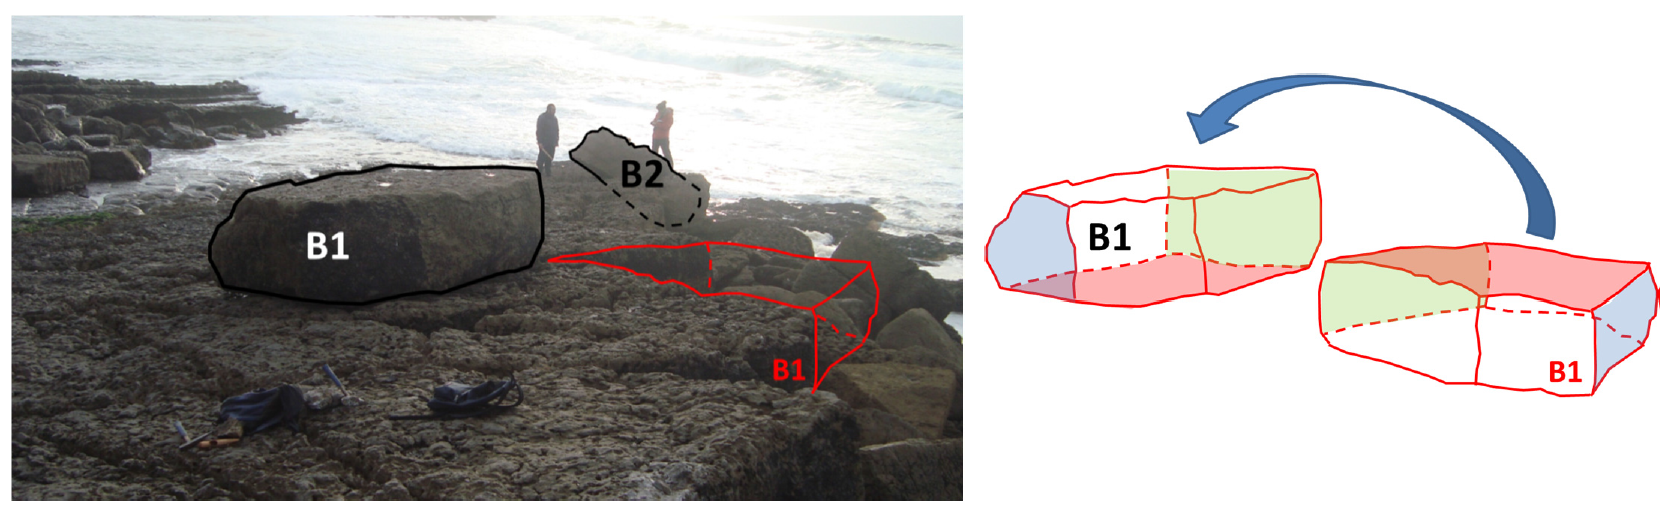
\includegraphics[width=0.85\linewidth]{Figures/6.Chapter/boulders_exp} 
	\caption{Praia das Ma\c{c}\~{a}s, Portugal. Boulder identification and orientation. \cite{Oliveira-2011}}
	\label{fig:boulders_exp} 
\end{figure}
%

Boulder B1 is $2.80\times2.0\times1.0$ m and weighs approximately 14 ton. It appears to have suffered a rotation and a small translation from the initial position. In this exploratory Section, the proposed model is applied as an inverse-problem, attempting to reproduce the dislodgement of megaclast, i.e, it is hypothesized that the pattern of deposition may be partially explained by actually modeling specific events in real geometries, attempting to recover the final observed state. 

The geometry of the problem is idealized but represents the key features of the overhanging layers related with fractures, bedding and differential erosion of sub-horizontal layers that originated block B1. In plan view, concave and convex coastline shapes are tested to assess the influence of momentum accumulation. A paddle with prescribed motion was used to generate a wave with $40\;m$ wavelength and $15\;m$ height, reproducing a large storm wave that breaks at the beach section. The lateral dimension is periodic to avoid any wall effects and the $2.84\times10^6$ particles are a result of $Dp=0.10\;m$ resolution, forcing 13 h long computations for 25 s events. The megaclast is assumed to be homogeneous limestone, with $E=4.5\times10^8 Nm^{-2}$, $\nu=0.15$ and $\mu=0.60$. Figures \ref{fig:boulders_I} to \ref{fig:boulders_IV} show the evolution of the system as the wave impacts the overhanging boulder.

%
\begin{figure}[ht!]
	\centering
	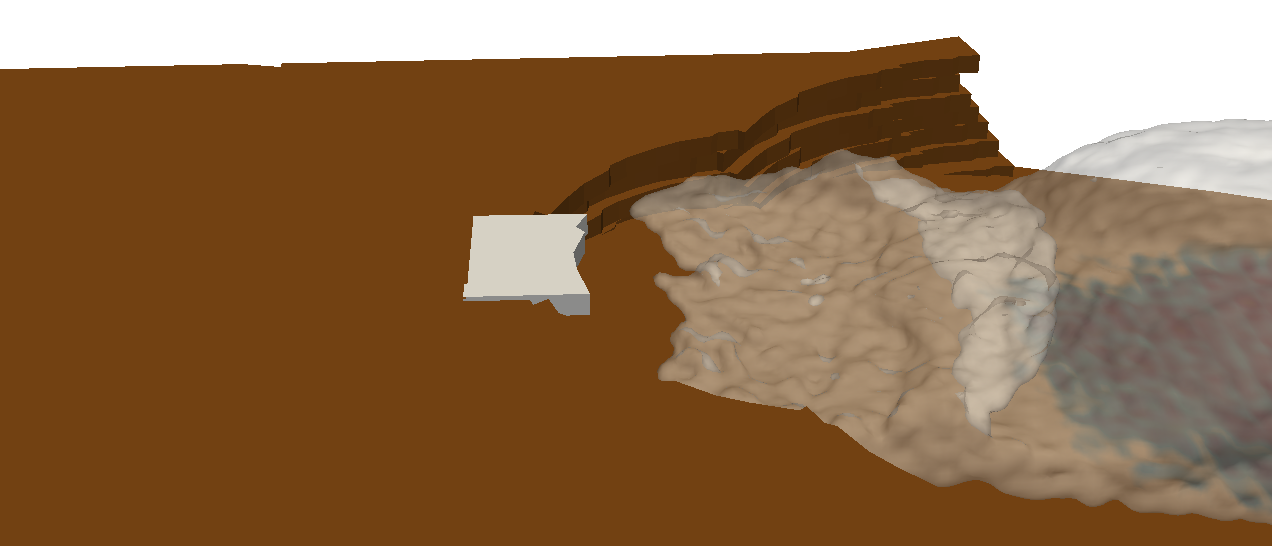
\includegraphics[width=0.42\linewidth]{Figures/6.Chapter/concave_105} 
	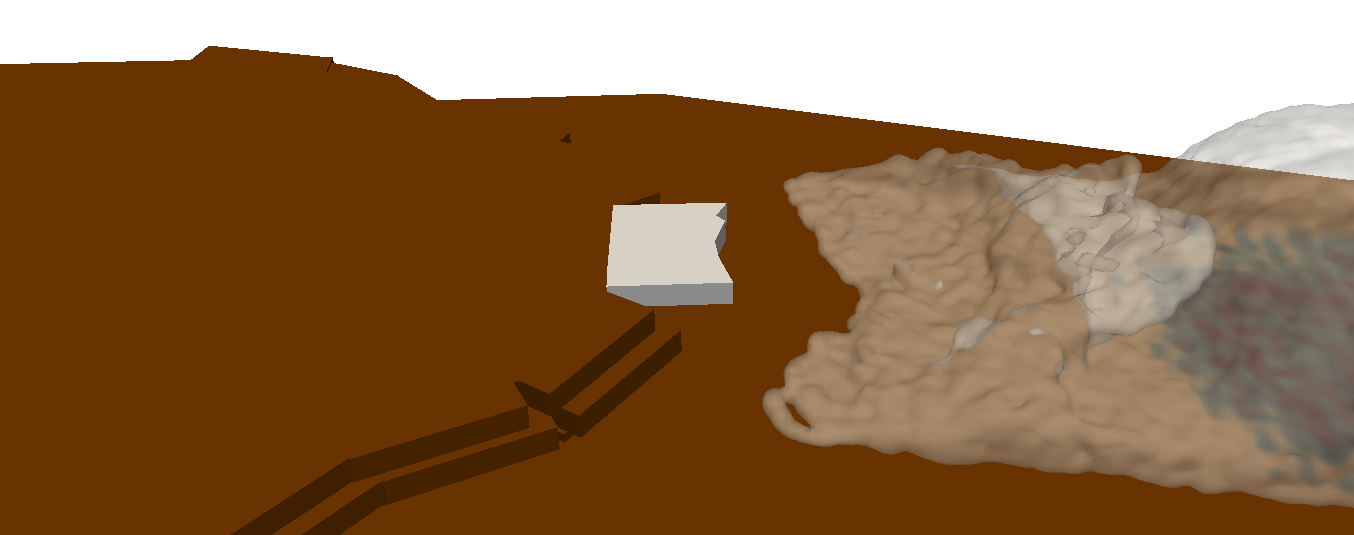
\includegraphics[width=0.42\linewidth]{Figures/6.Chapter/convex_105}
	%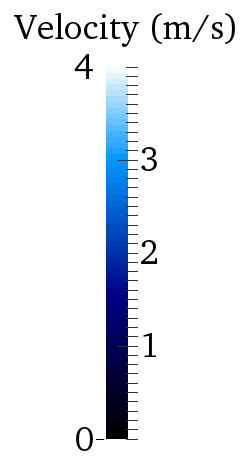
\includegraphics[width=0.13\linewidth]{Figures/6.Chapter/label} 
	\caption{Concave and convex geometries, $t=10.5$ s.}
	\label{fig:boulders_I} 
\end{figure}
%

%
\begin{figure}[ht!]
	\centering
	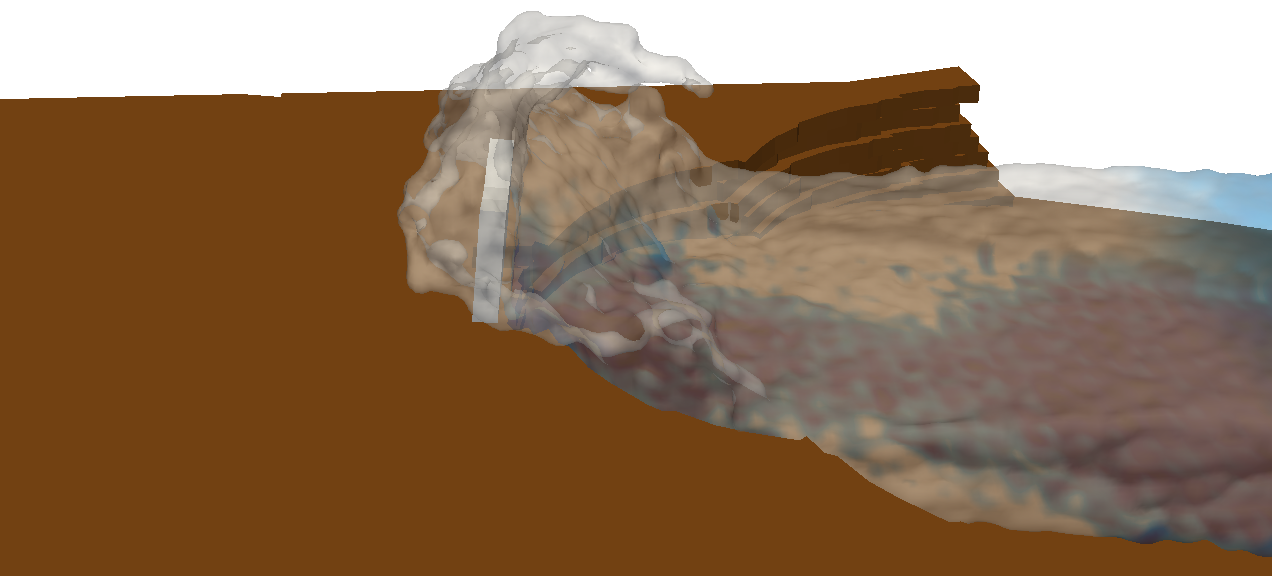
\includegraphics[width=0.42\linewidth]{Figures/6.Chapter/concave_115} 
	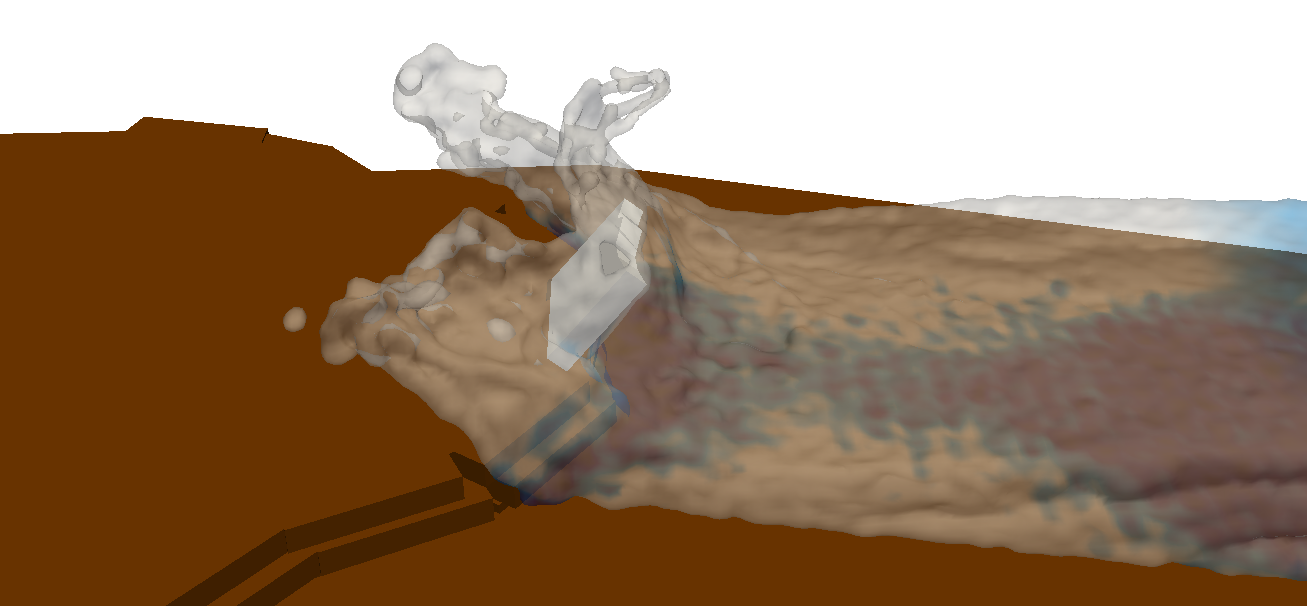
\includegraphics[width=0.42\linewidth]{Figures/6.Chapter/convex_115} 
	%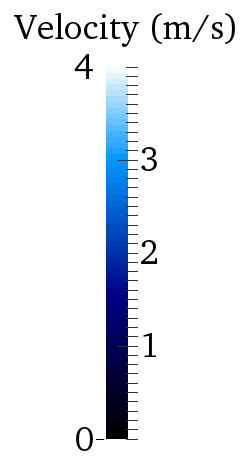
\includegraphics[width=0.13\linewidth]{Figures/6.Chapter/label} 
	\caption{Concave and convex geometries, $t=11.5$ s.}
	\label{fig:boulders_II} 
\end{figure}
%

%
\begin{figure}[ht!]
	\centering
	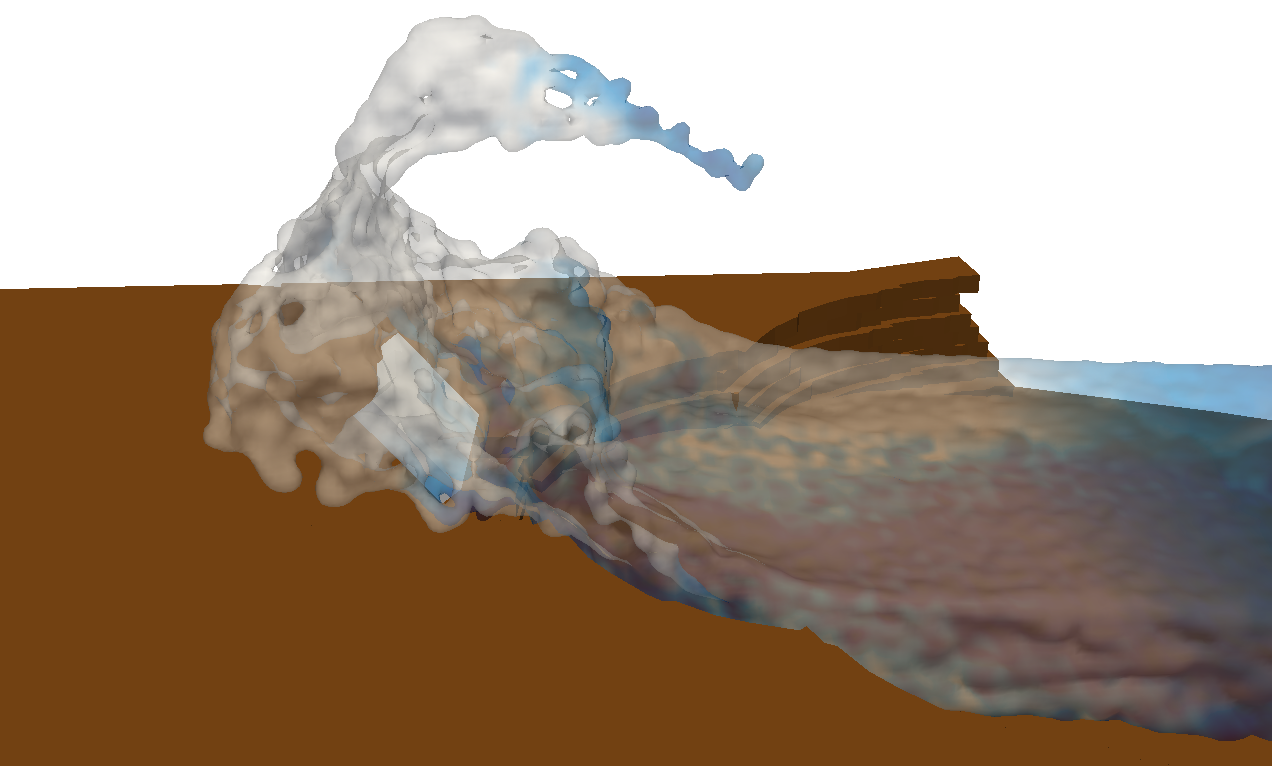
\includegraphics[width=0.42\linewidth]{Figures/6.Chapter/concave_120} 
	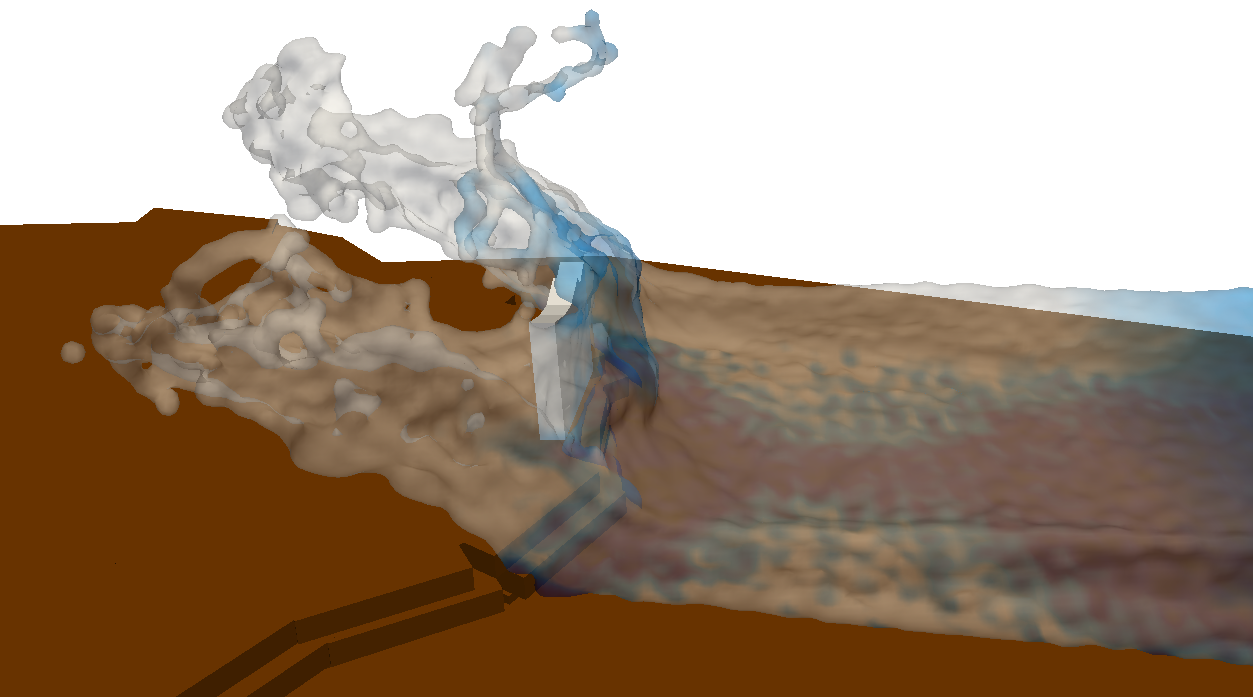
\includegraphics[width=0.42\linewidth]{Figures/6.Chapter/convex_120} 
	%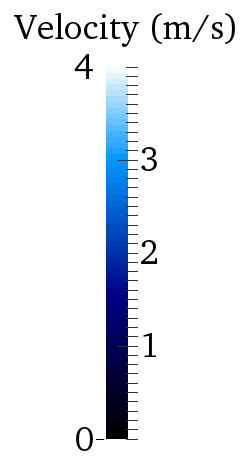
\includegraphics[width=0.13\linewidth]{Figures/6.Chapter/label} 
	\caption{Concave and convex geometries, $t=12.0$ s.}
	\label{fig:boulders_III} 
\end{figure}
%

%
\begin{figure}[ht!]
	\centering
	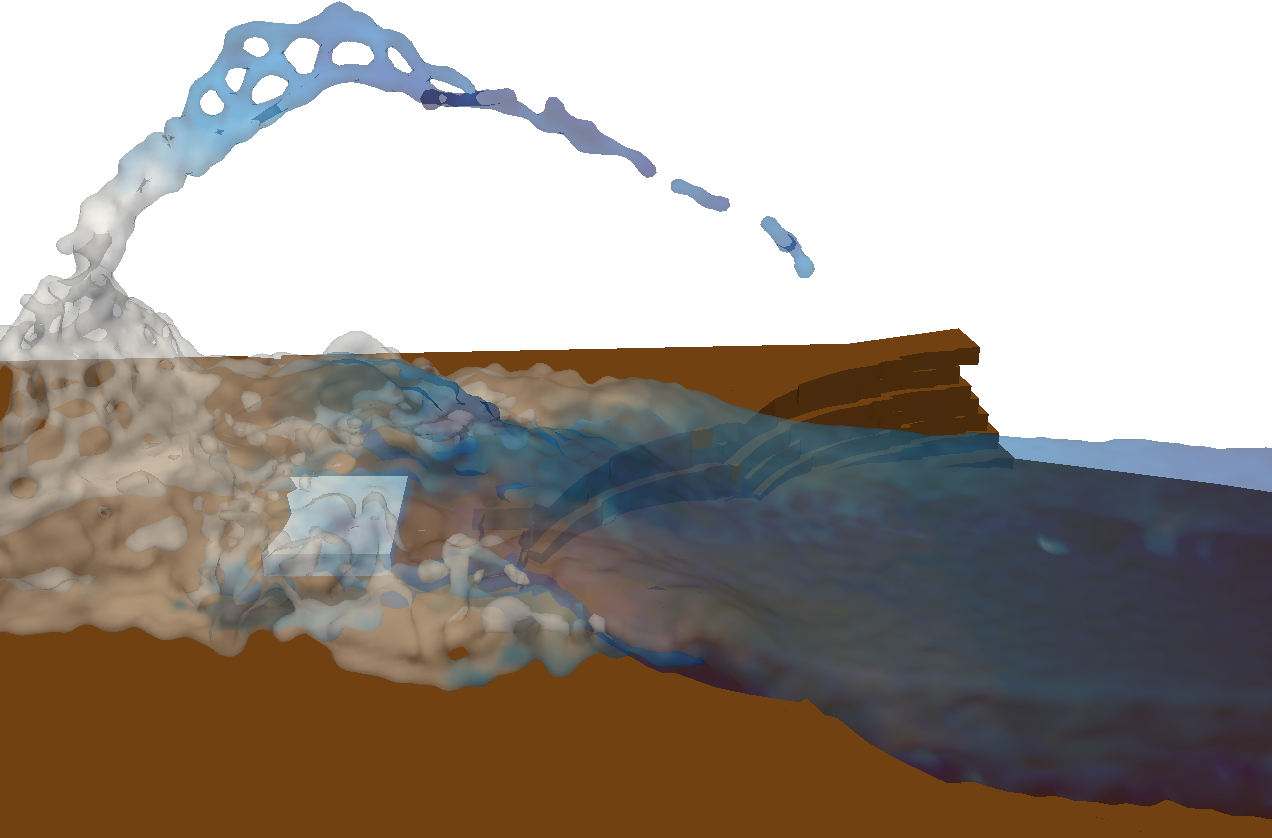
\includegraphics[width=0.42\linewidth]{Figures/6.Chapter/concave_130} 
	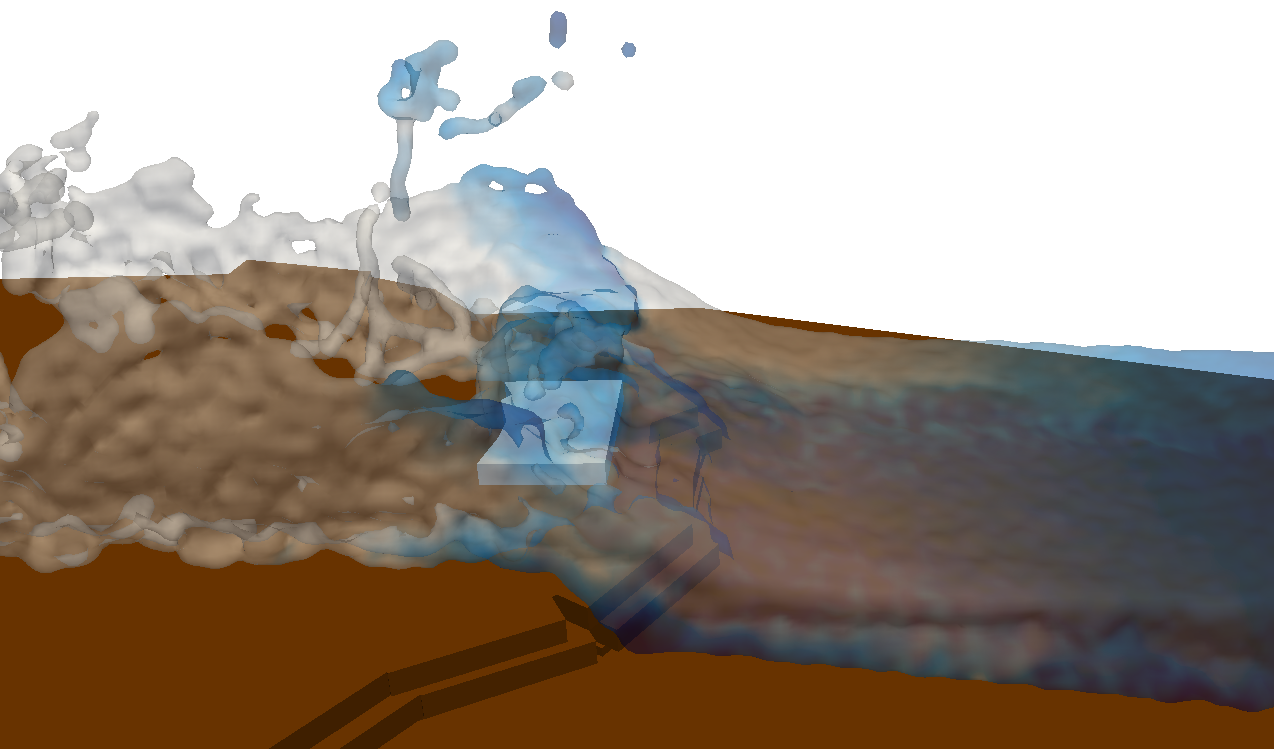
\includegraphics[width=0.42\linewidth]{Figures/6.Chapter/convex_130} 
	%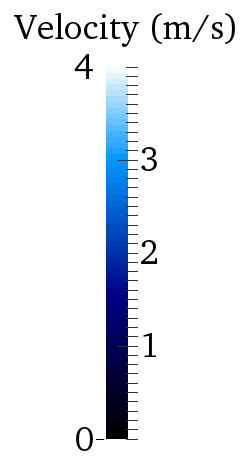
\includegraphics[width=0.13\linewidth]{Figures/6.Chapter/label} 
	\caption{Concave and convex geometries, $t=13.0$ s.}
	\label{fig:boulders_IV} 
\end{figure}
%

Differences in concave to convex geometries are within expectation: momentum seems to be concentrated in the concave case, as the megaclast rotates faster (Figure \ref{fig:boulders_III}) and is transported around $1$ m further comparing to the convex case. 

Another fundamental aspect of the phenomenon is overhanging versus supported geometry. Two contact forces are responsible for the dislodgement of the boulders: pressure and momentum flux. The main working force is the momentum flux, but the work of both for the boulder movement is proportional to the area exposed. Figures \ref{fig:boulders_V} and \ref{fig:boulders_VI} show the pressure field on the impact locus. 

%
\begin{figure}[ht!]
	\centering
	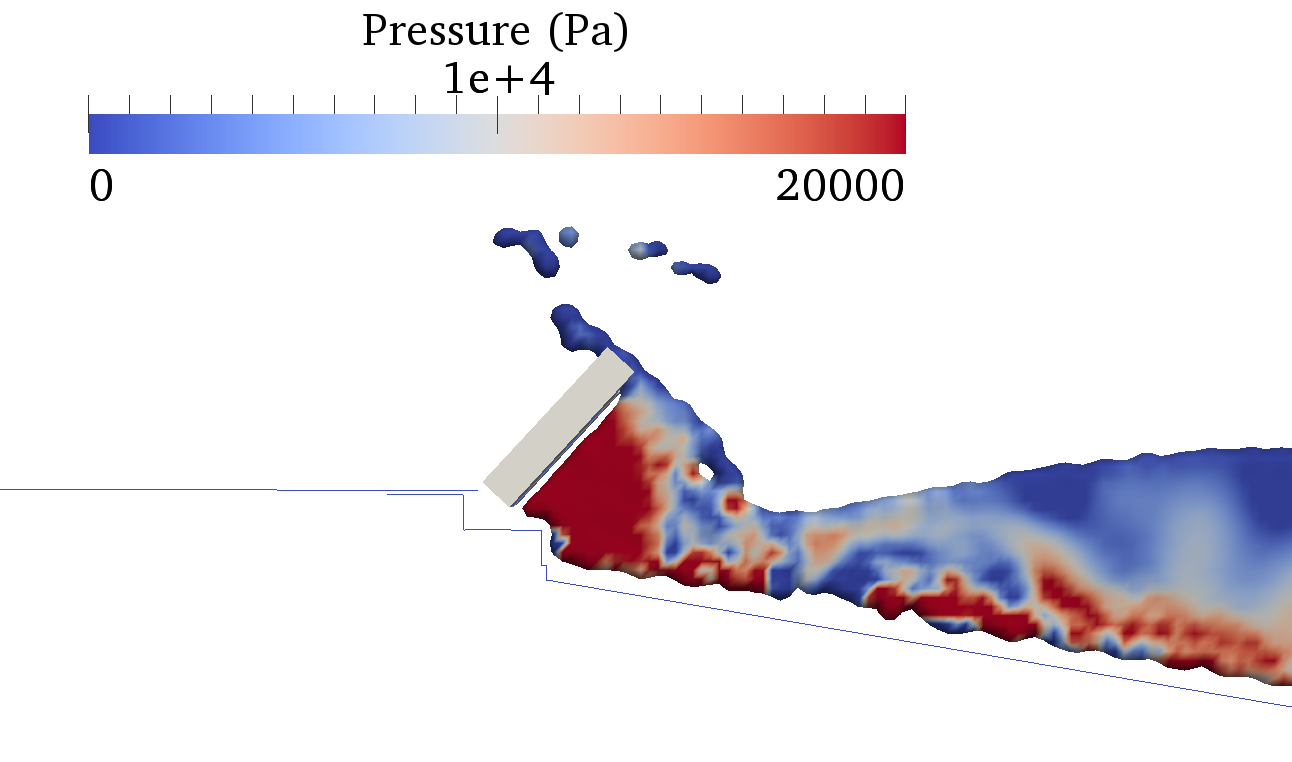
\includegraphics[width=0.48\linewidth]{Figures/6.Chapter/2D_press_norm_I} 
	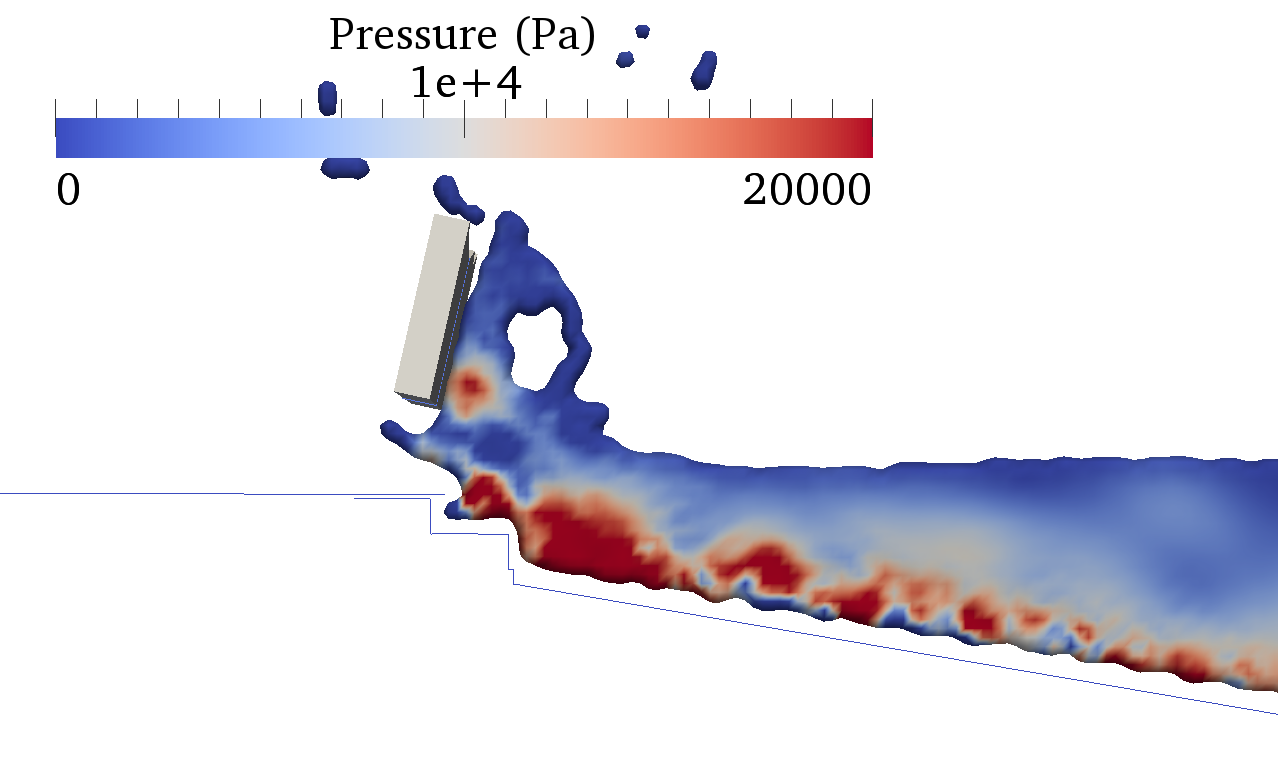
\includegraphics[width=0.48\linewidth]{Figures/6.Chapter/2D_press_norm_II}
	\caption{Concave geometry. Vertical plane over domain axis. Overhanging case. Left-$t=10.9$ s, right-$t=11.5$ s.}
	\label{fig:boulders_V} 
\end{figure}
%

%
\begin{figure}[ht!]
	\centering
	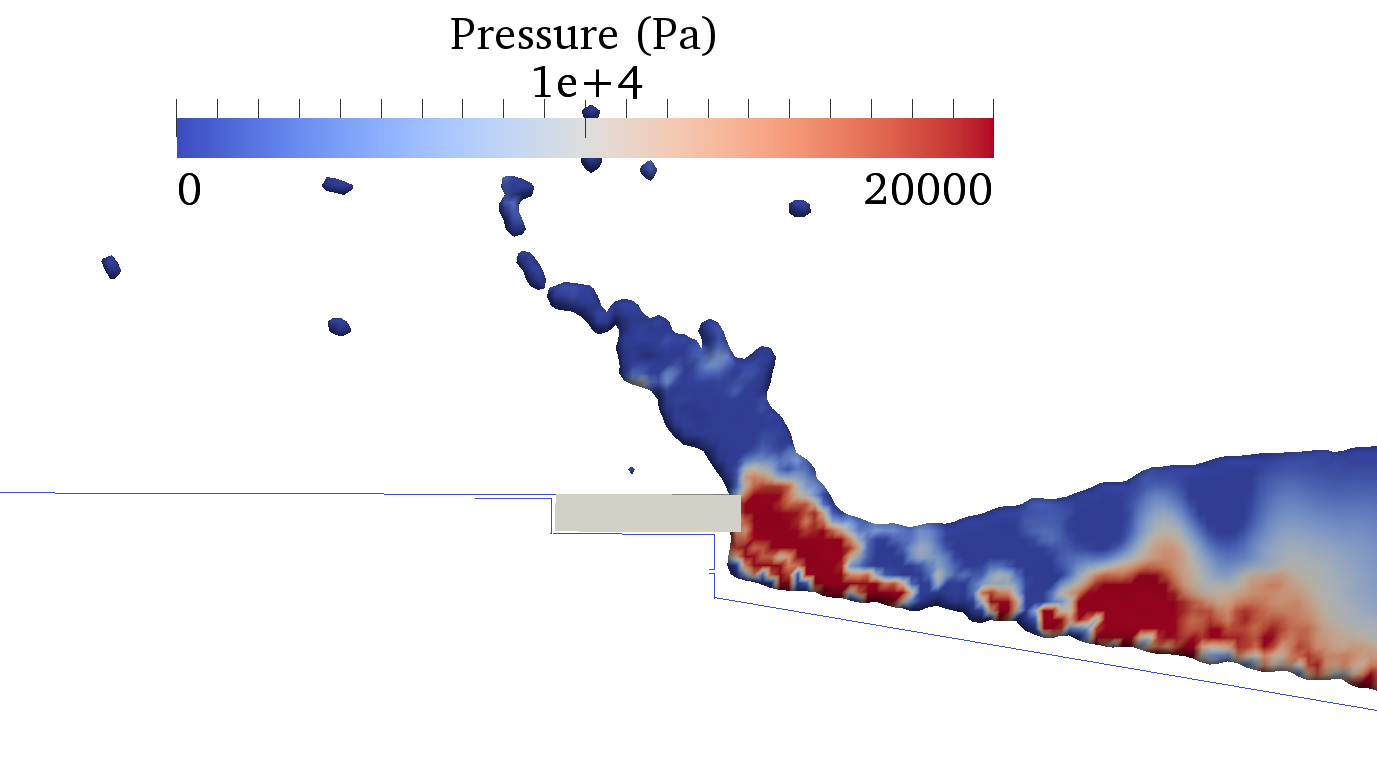
\includegraphics[width=0.48\linewidth]{Figures/6.Chapter/2D_press_flat}
	\caption{Concave geometry. Vertical plane over domain axis. Supported case. $t=11.5$ s.}
	\label{fig:boulders_VI} 
\end{figure}
%

As expected, a significant pressure build-up occurs in the impact locus. The cavity in the overhanging configuration allows the contact forces to produce work on the boulder, in contrast with the supported case.

The local (micro to meso-scale) geomorphological conditions in rocky coastal contexts strongly control the capability of waves to entrain and transport large particles upward and inland. The flow modulation induced by these features is not adequately addressed by conventional numerical solutions and requires the application of models capable of explicitly resolving the momentum transfer between phases and take into account complex geometrical considerations.





%%%%%%%%%%%%%%%%%%%%%%%%%%%%%%%%%%%%%%%%%%%%%%%%%%%%%%%%%%%
\section{Sines Port}
\label{sec:sines}

The Sines Container Terminal, called Terminal XXI, is a major infrastructure in the Portuguese coast, currently capable of handling 1,100,000 TEU, with plans of extending up to 1,700,000 TEU. As mentioned in Section \ref{sec:coastal_geomorphology} Portugal's Atlantic coast, especially southwards of Lisbon, is subject to a non negligible risk of tsunami waves caused by seismic events that occur offshore. These results show the influence of a wave in stacked containers and other obstacles in a reduced subsection of the quay, detailed in Figure \ref{fig:sines_map}.

%
\begin{figure}[ht!]
	\centering
	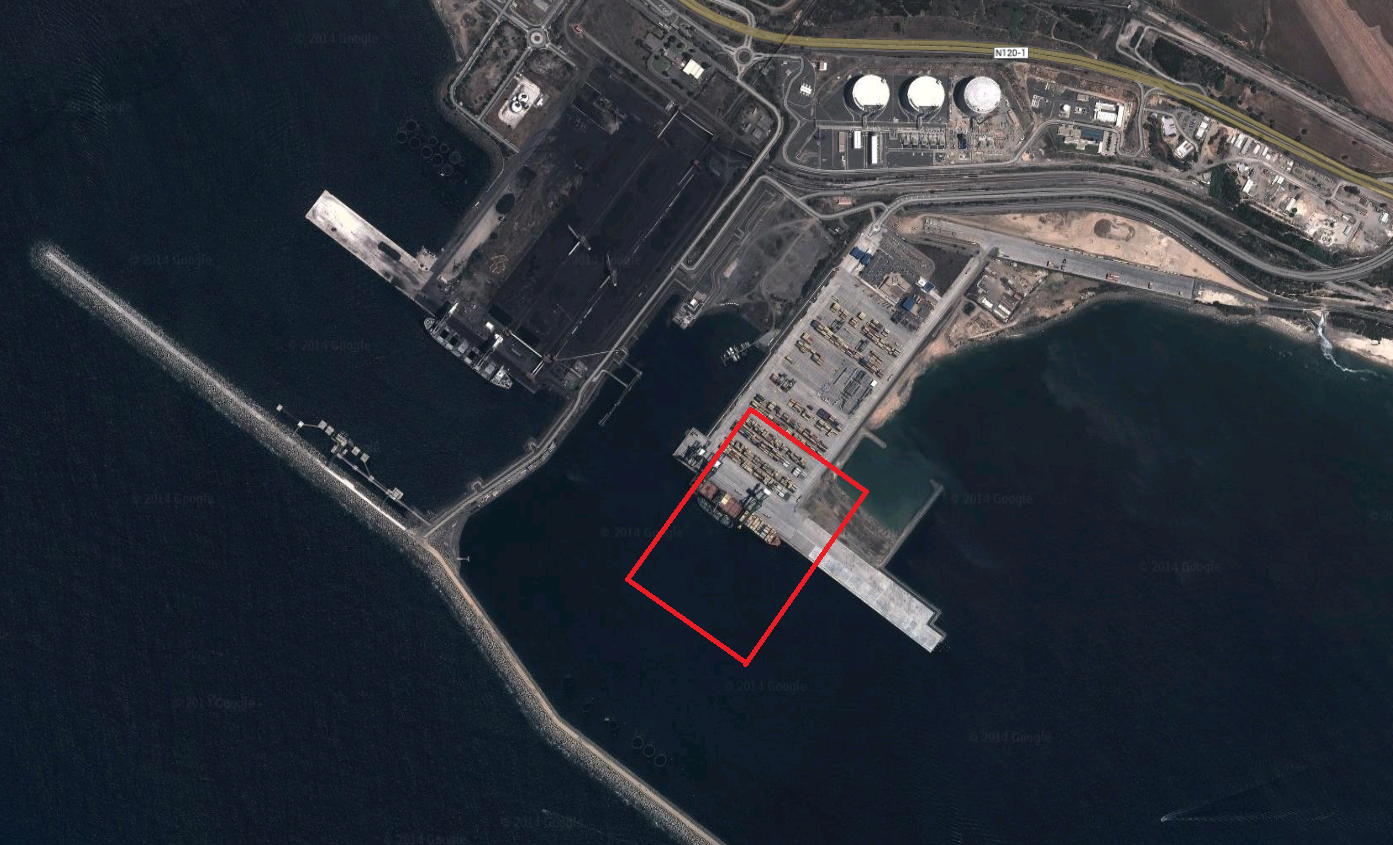
\includegraphics[width=0.80\linewidth]{Figures/6.Chapter/map_sines_domain} 
	\caption{Aerial view of the Terminal XXI of the Sines Port. Red square indicates the computational domain.}
	\label{fig:sines_map} 
\end{figure}
%

The section of the harbor is partially protected by a breakwater to the east, neglected in this case to simplify the behavior of the wave on the area of interest. The chosen domain originates an excess of $12\times10^6$ particles, for a $Dp=0.5$ m, resulting in a 57 h long computation for the 60 s event. The type of wave to be generated must observe some limitations, since the wavelength must be less than the domain extent, to avoid issues at the boundaries. As stated, the breakwater is disregarded, not having any influence in the simulated wave. The equations used to generate the solitary wave were \citep{Dean-Dalrymple-1991}

%
\begin{equation} \label{eq:solitary_wave}
	V=\sqrt{\frac{4D^3}{3H}}; \;\;\; \eta(x')=\frac{D}{\cosh^2\left(\frac{x'}{V}\right)} ; \;\;\; v(x')=\eta(x')\sqrt{\frac{-g}{D}}
\end{equation}
%
where $D$ is the fluid depth, $H$ is the maximum wave height, $\eta=D+H$ and $x'$ is a coordinate normal to the wave axis measured from the wave apex. Propagating a wave from a synthetic tsunami generates a wave height of $15$ m, corresponding, according to equations \eqref{eq:solitary_wave} to a top velocity of about $5.6\;\text{ms}^{-1}$ and wavelength of approximately $130$ m, against the expected several hundreds of an actual tsunami \cite{mavbaptista-2011}. The initial conditions of the system can be seen in Figure \ref{fig:sines_ini_cond}.

%
\begin{figure}[ht!]
	\centering
	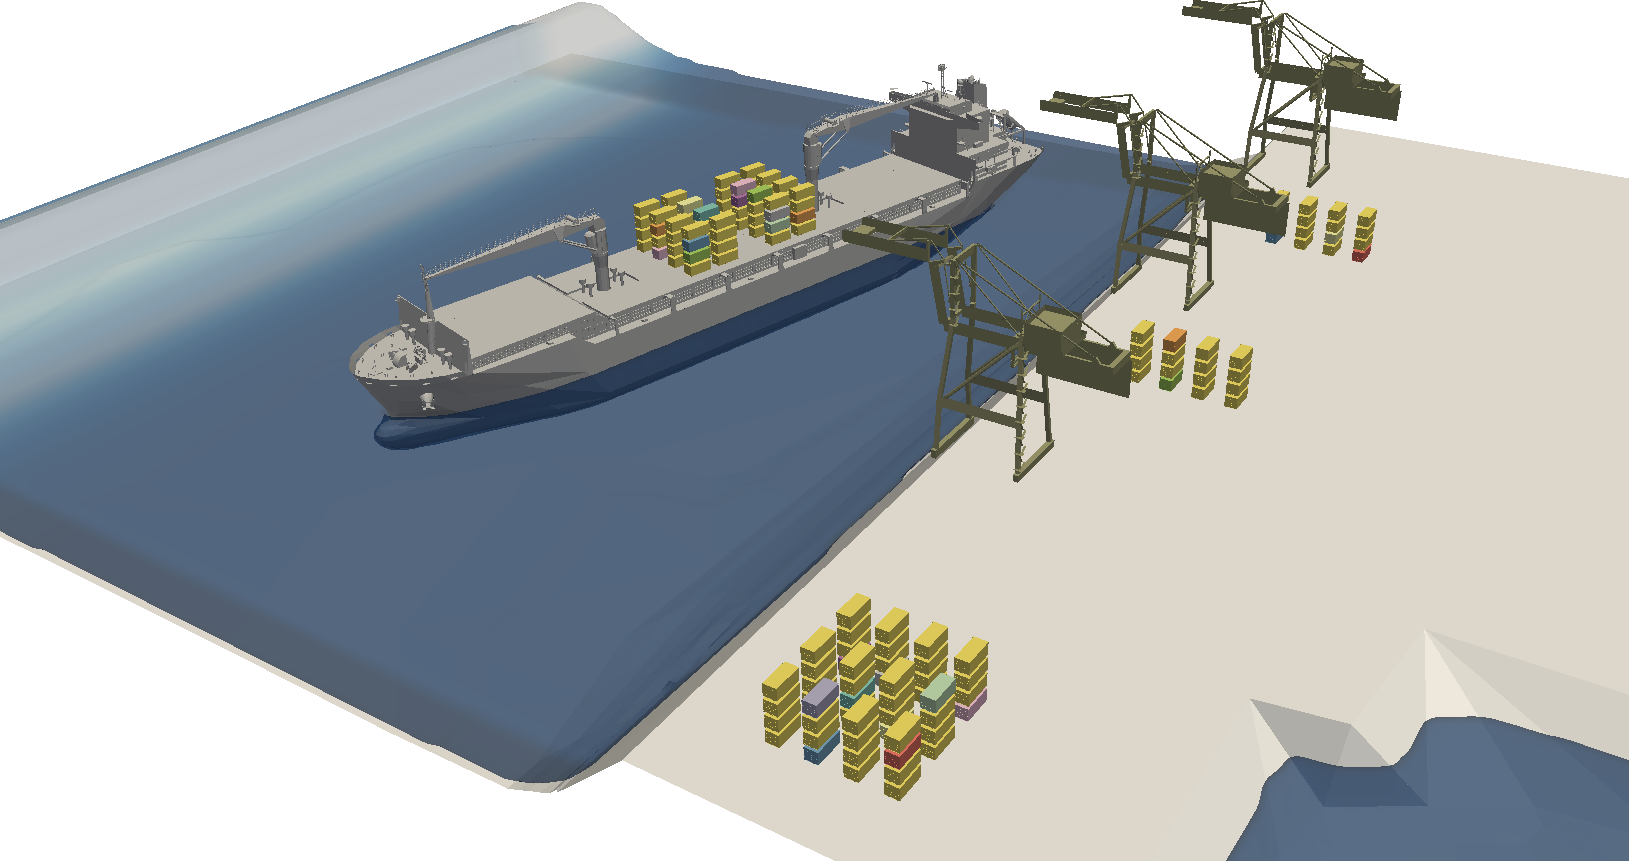
\includegraphics[width=0.95\linewidth]{Figures/6.Chapter/sines_ini_cond_II} 
	\caption{Initial conditions of the system.}
	\label{fig:sines_ini_cond} 
\end{figure}
%

The direction of the wave is normal to the quay wall structure. A cargo ship is placed in the domain, as well as a total of 143 ship containers, 64 of which on the ship. The ship has a density of $\rho=0.3\rho_{w}$ and the center of gravity was made to coincide with that of the actual ship. The geometry consists of the actual 3D scan of a ship hull, and was discretized as hollow, since no information on the internal structure of the ship is available and it would result in the most accurate inertia tensor. The ship containers are assumed half-full and as such with a $\rho=2.5\rho_{w}$ density. Each individual body has 6 degrees of freedom, no restrictions are applied, and are made of steel. The gantry cranes are also made of steel but are represented as fixed boundaries and the terrain was considered limestone. Table \ref{tab:material_props_sines} details the parameters used in the simulations. The \emph{CFL} constant was used as $C=0.2$, artificial viscosity with $\alpha=0.05$ and $h=\sqrt{3Dp^2}$.

%
\begin{table}[h]
\centering
\begin{tabular}{l|l|llll}
 & Material & $E\;[Nm^{-2}]$ & $\nu_p\;[-]$  & $e\;[-]$ & $\mu_f\;[-]$\\ \hline
Containers/Gantry cranes/Ship & Steel & $200\times10^9$ & $0.30$ & $0.85$ & $0.55$ \\
Terrain & Limestone & $4.5\times10^9$ & $0.15$ & $0.80$ & $0.60$
\end{tabular}
\caption{Young modulus, Poisson coefficient, restitution coefficient and friction coefficient used in the simulations.}
\label{tab:material_props_sines}
\end{table}
%

The wave travels approximately $7$ s until it hits the ship. The large acceleration immediately causes the instabilization of the most forward container stacks. Figure \ref{fig:sines_t38} represents the beginning of the ship motion and one can notice the beginning of the instabilization of the containers on the port-side.
\begin{figure}[H]
	\centering
	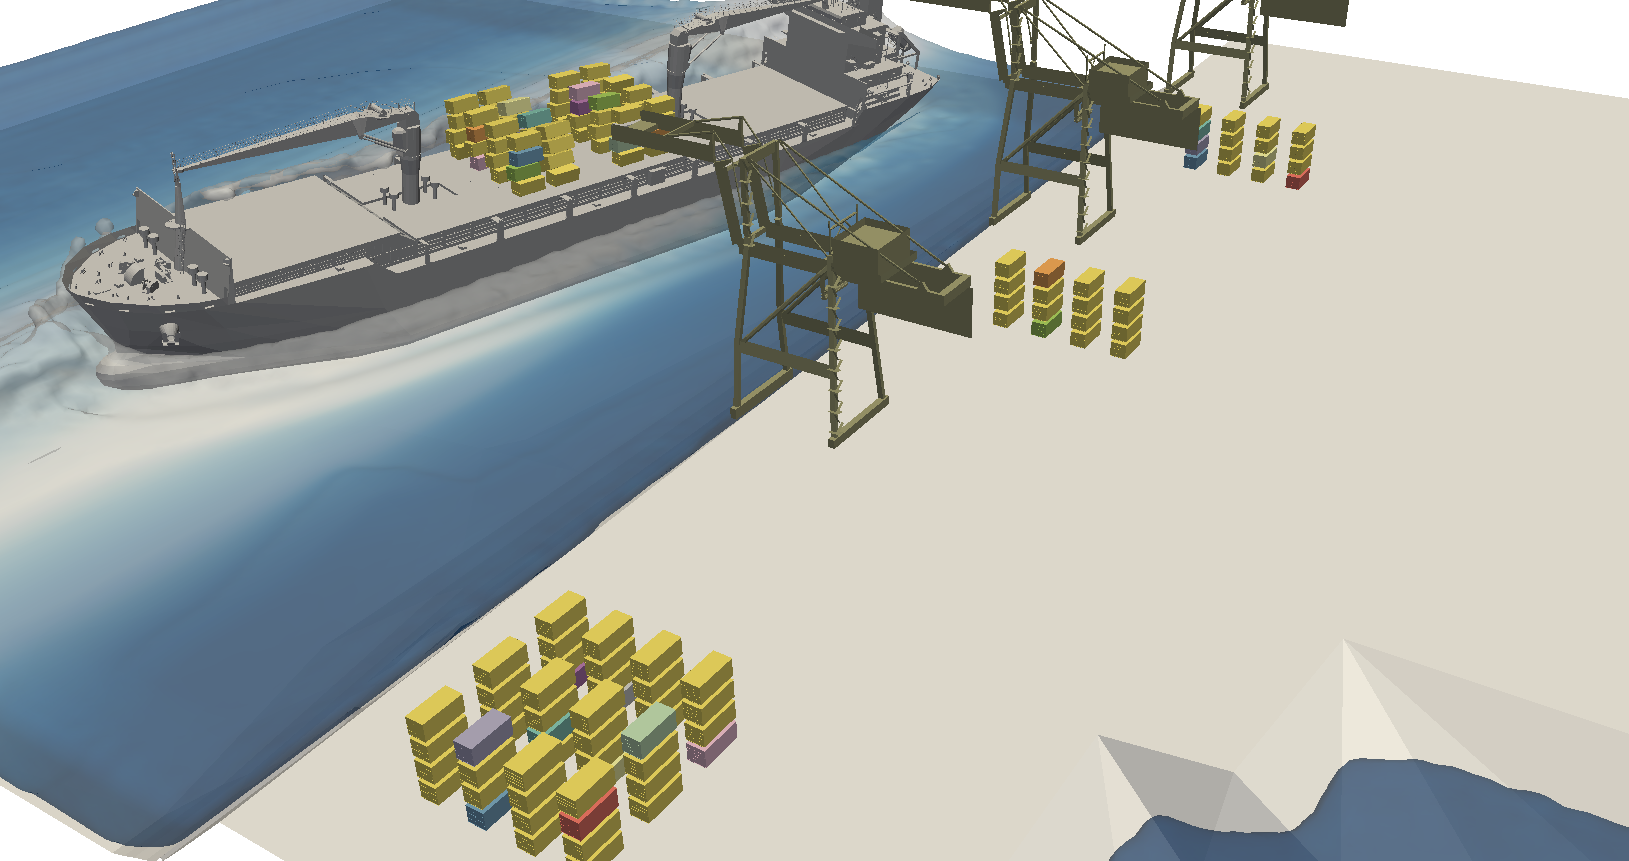
\includegraphics[width=0.95\linewidth]{Figures/6.Chapter/sines_t38_II} 
	\caption{General view of the application case, $t=7.6$ s.}
	\label{fig:sines_t38} 
\end{figure}
%

Figure \ref{fig:sines_t60}, at $t=12.0$ s, shows the container motion after the wave passage. 
\begin{figure}[H]
	\centering
	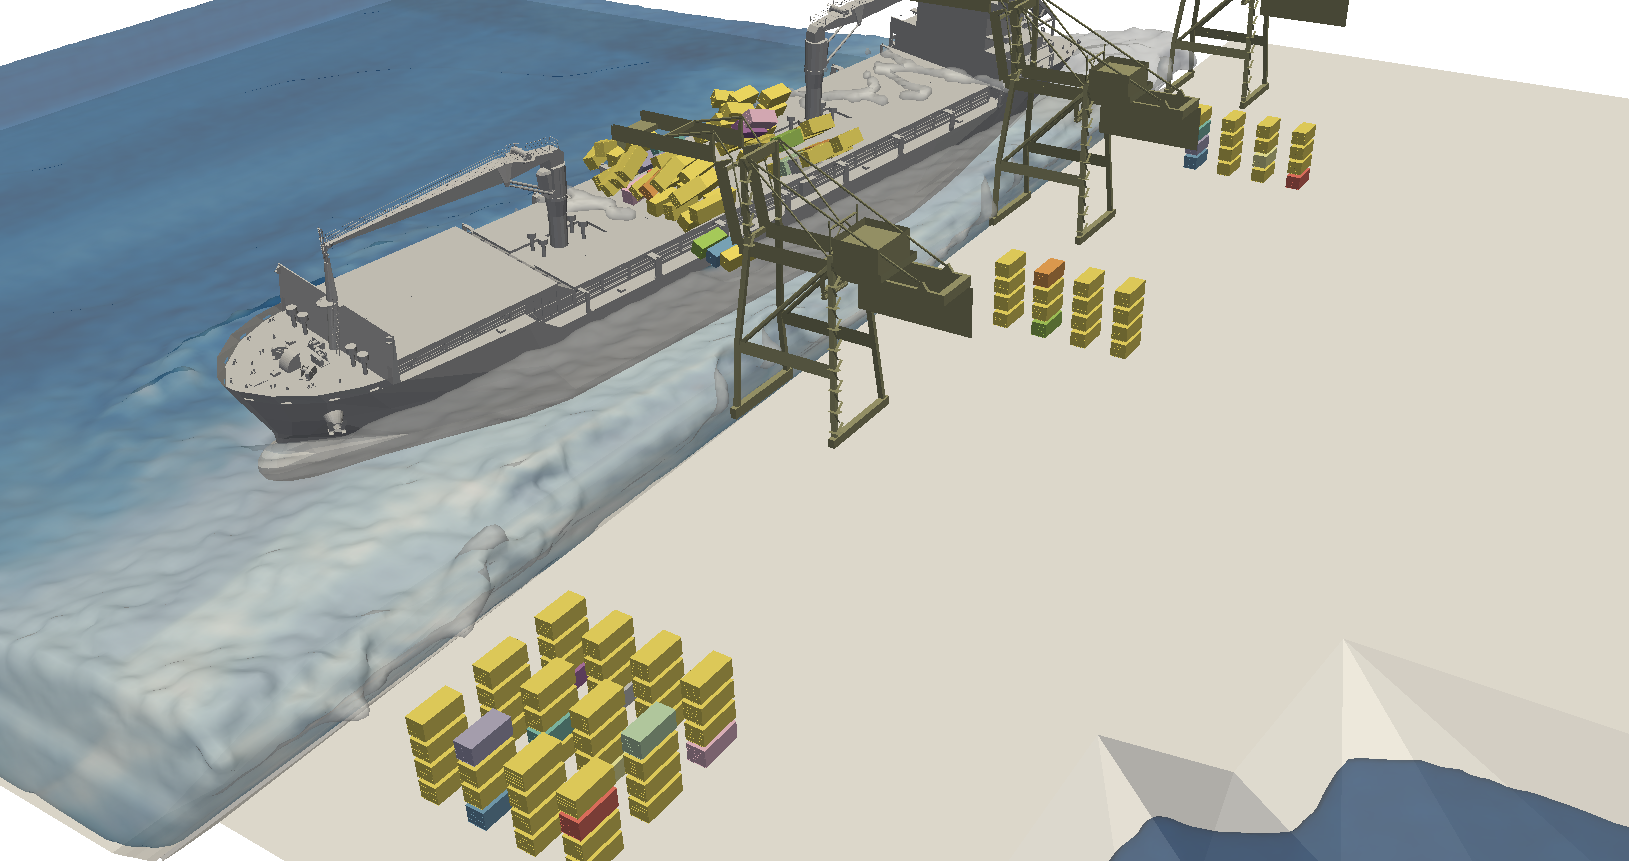
\includegraphics[width=0.95\linewidth]{Figures/6.Chapter/sines_t60_II} 
	\caption{General view of the application case, $t=12.0$ s.}
	\label{fig:sines_t60} 
\end{figure}
%

Figures \ref{fig:sines_t70} and \ref{fig:sines_t90}, at $t=14.0$ s and $t=18.0$ s, respectively, demonstrate the wave overtopping the quay and deforming at the base of the gantry cranes and the container stacks. 
\begin{figure}[H]
	\centering
	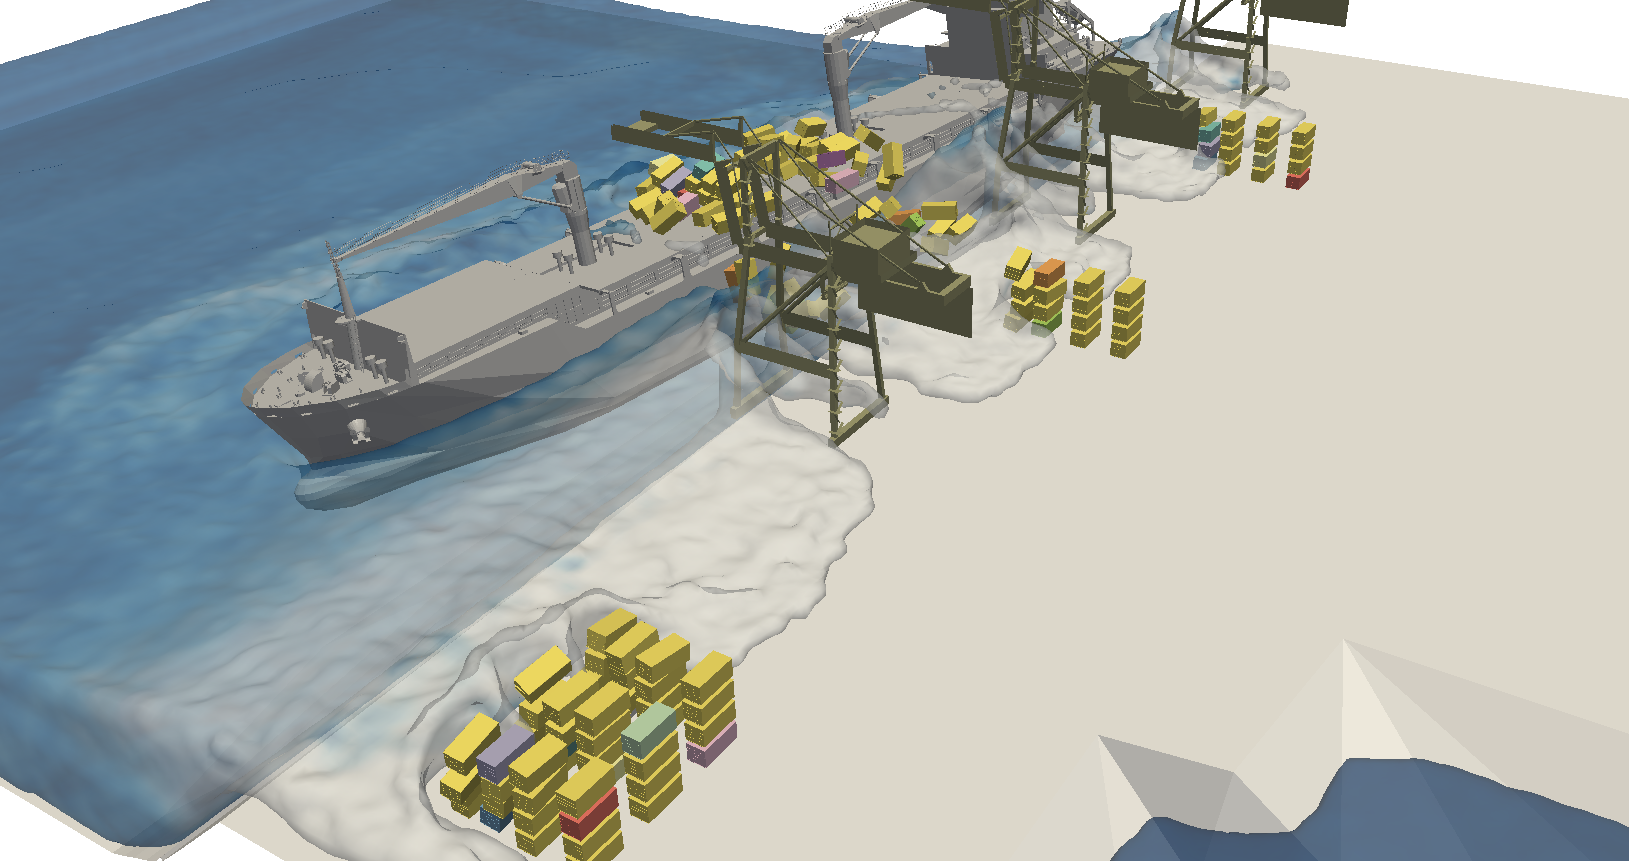
\includegraphics[width=0.95\linewidth]{Figures/6.Chapter/sines_t70_II} 
	\caption{General view of the application case, $t=14.0$ s.}
	\label{fig:sines_t70} 
\end{figure}
%
%
\begin{figure}[H]
	\centering
	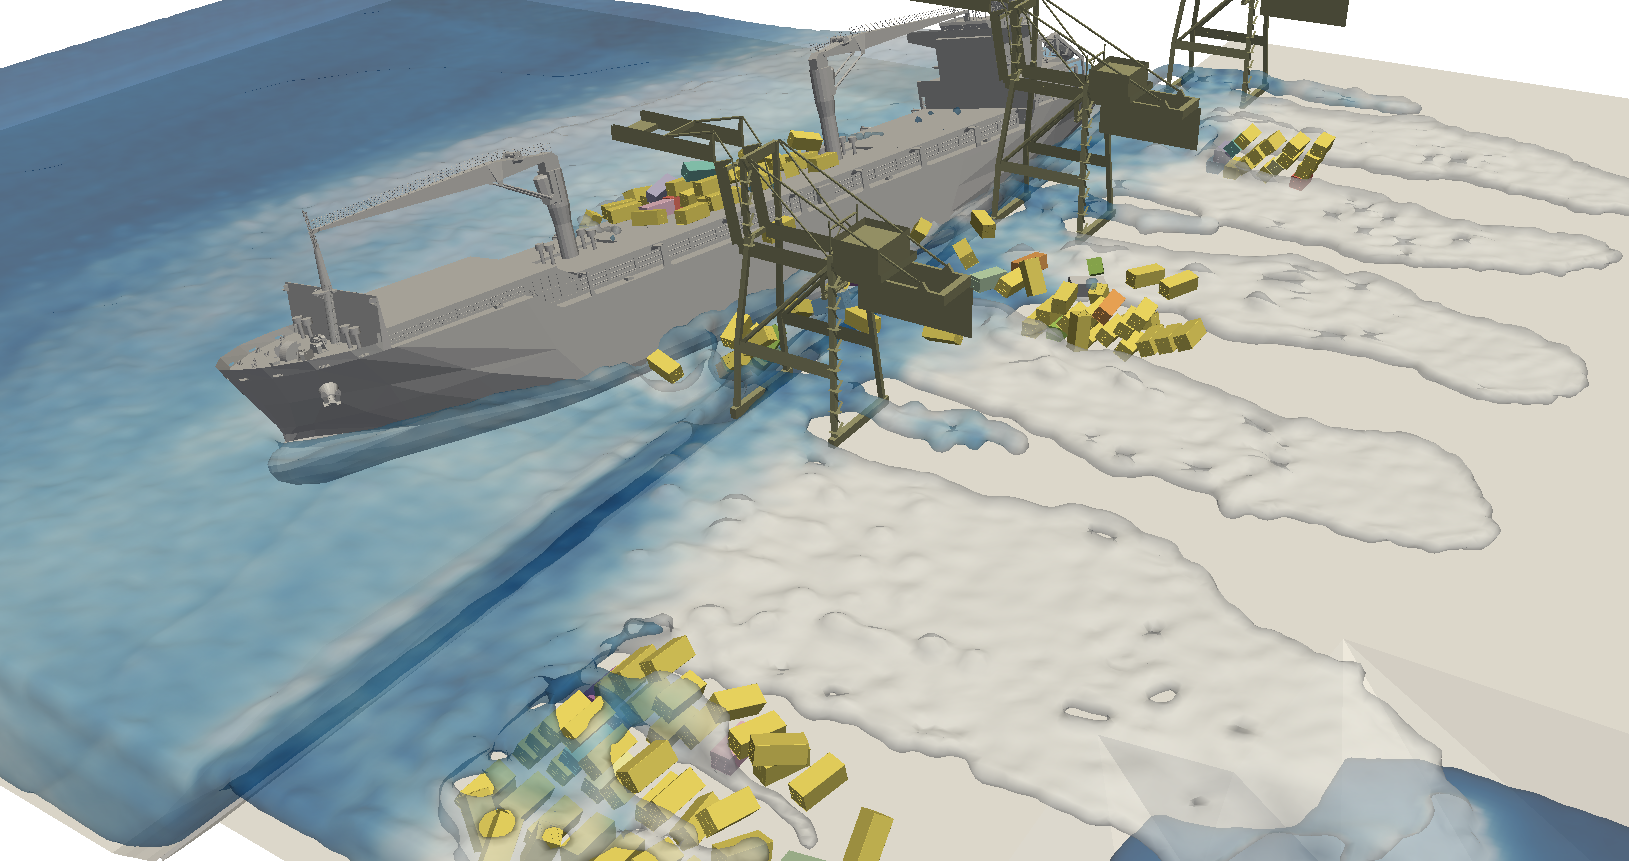
\includegraphics[width=0.95\linewidth]{Figures/6.Chapter/sines_t90_II} 
	\caption{General view of the application case, $t=18.0$ s.}
	\label{fig:sines_t90} 
\end{figure}
%
Instabilization of the piles is evident, with complex contact events being treated with no aberrant results. Containers initially aboard the ship are now in the water, most of them between the ship hull and the harbor structure.

Figure \ref{fig:sines_t300}, at $t=60.0$ s, show the state of the system at the end of simulated time.
\begin{figure}[H]
	\centering
	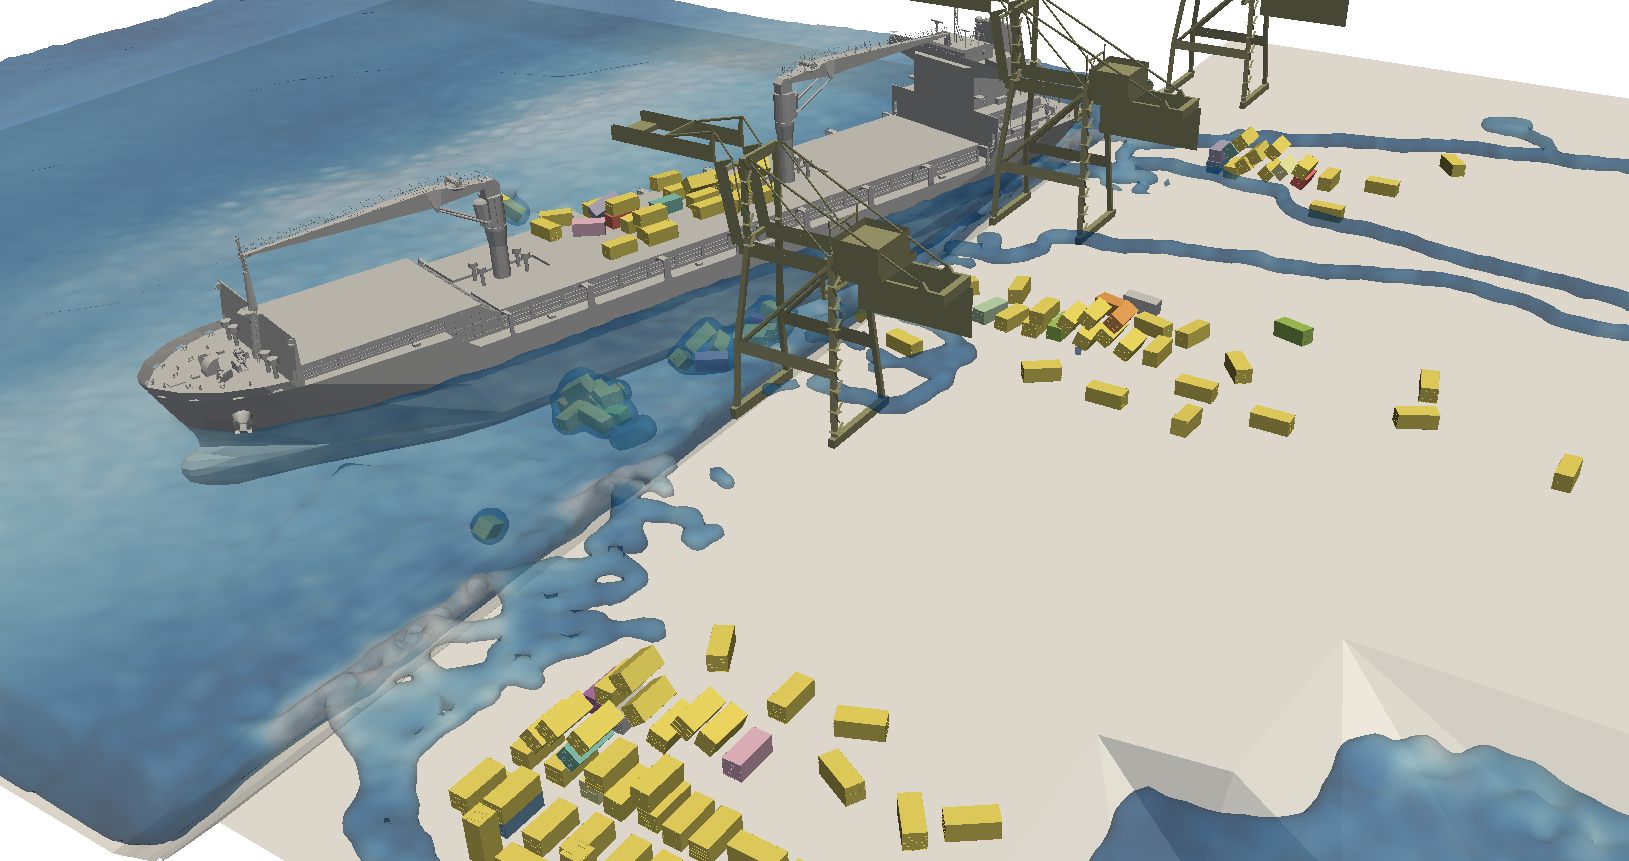
\includegraphics[width=0.95\linewidth]{Figures/6.Chapter/sines_t300_II} 
	\caption{General view of the application case, $t=60.0$ s.}
	\label{fig:sines_t300} 
\end{figure}
%
Some containers were dragged a considerable length, over $100\times$ its own characteristic dimensions. Large piles of containers can be seen, formed after the initial configurations were perturbed, since the wave did not have enough momentum to transport all the containers.

With a more detailed perspective over a set of containers, Figure \ref{fig:cont_t70}, at $t=14.0$ s, shows the instant immediately after wave impact. 
%
\begin{figure}[H]
	\centering
	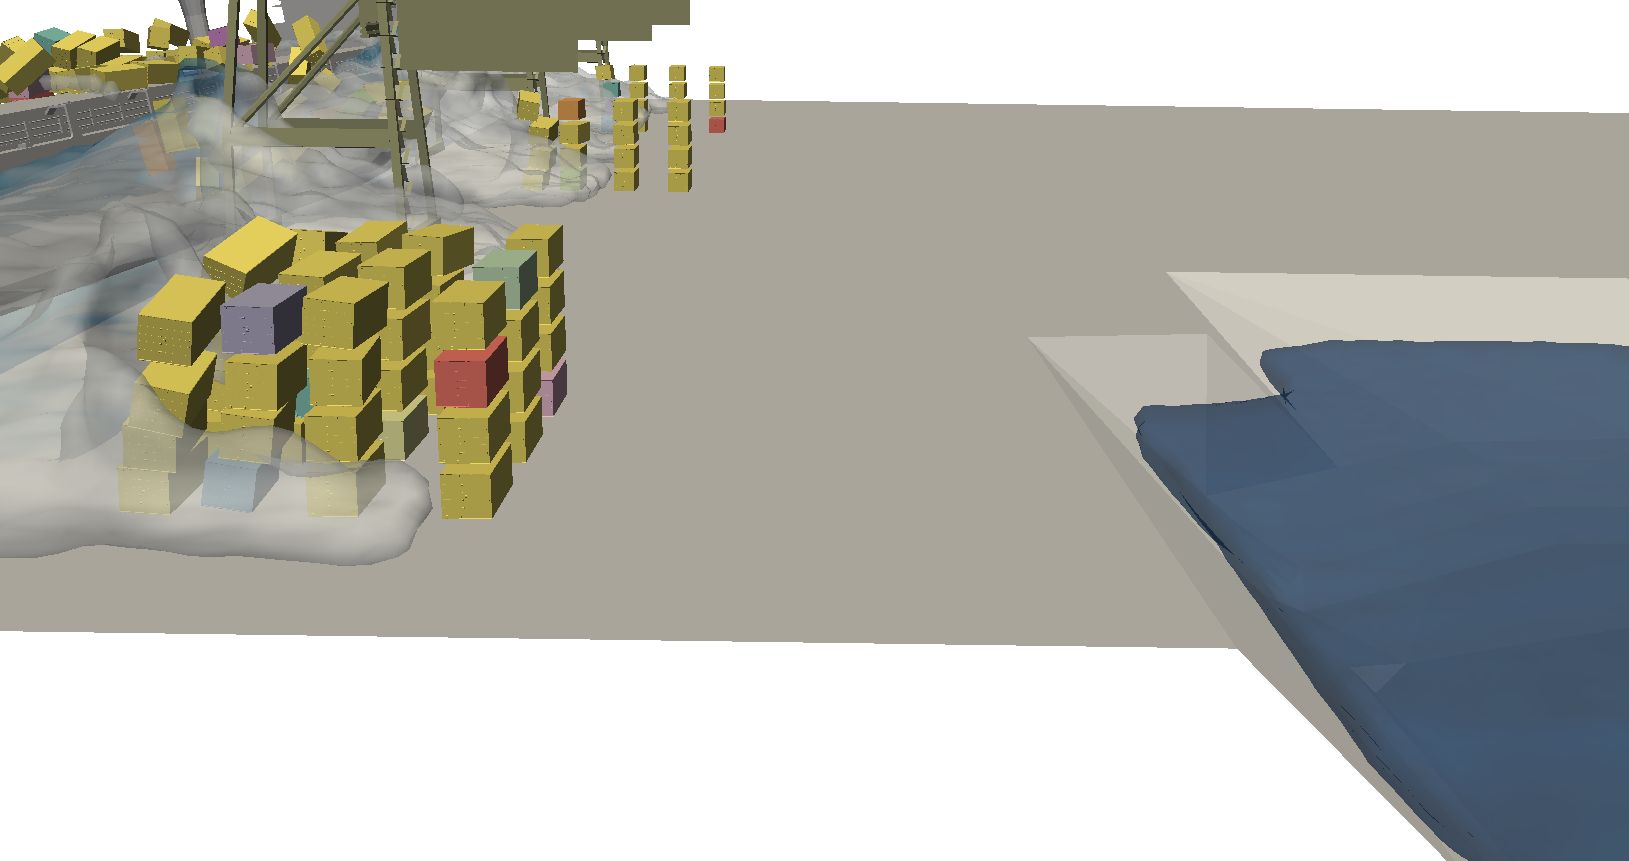
\includegraphics[width=0.95\linewidth]{Figures/6.Chapter/cont_t70} 
	\caption{Details of a set of container stacks, $t=14.0$ s.}
	\label{fig:cont_t70} 
\end{figure}
% 

Figures \ref{fig:cont_t80},\ref{fig:cont_t85} and \ref{fig:cont_t90} show the collapse of the set of containers due to the impact of the wave. Little motion of the containers is due to sustained transport, most of the momentum arises from the potential energy in the vertical pile and short contact forces due to the collisions. 
%
\begin{figure}[H]
	\centering
	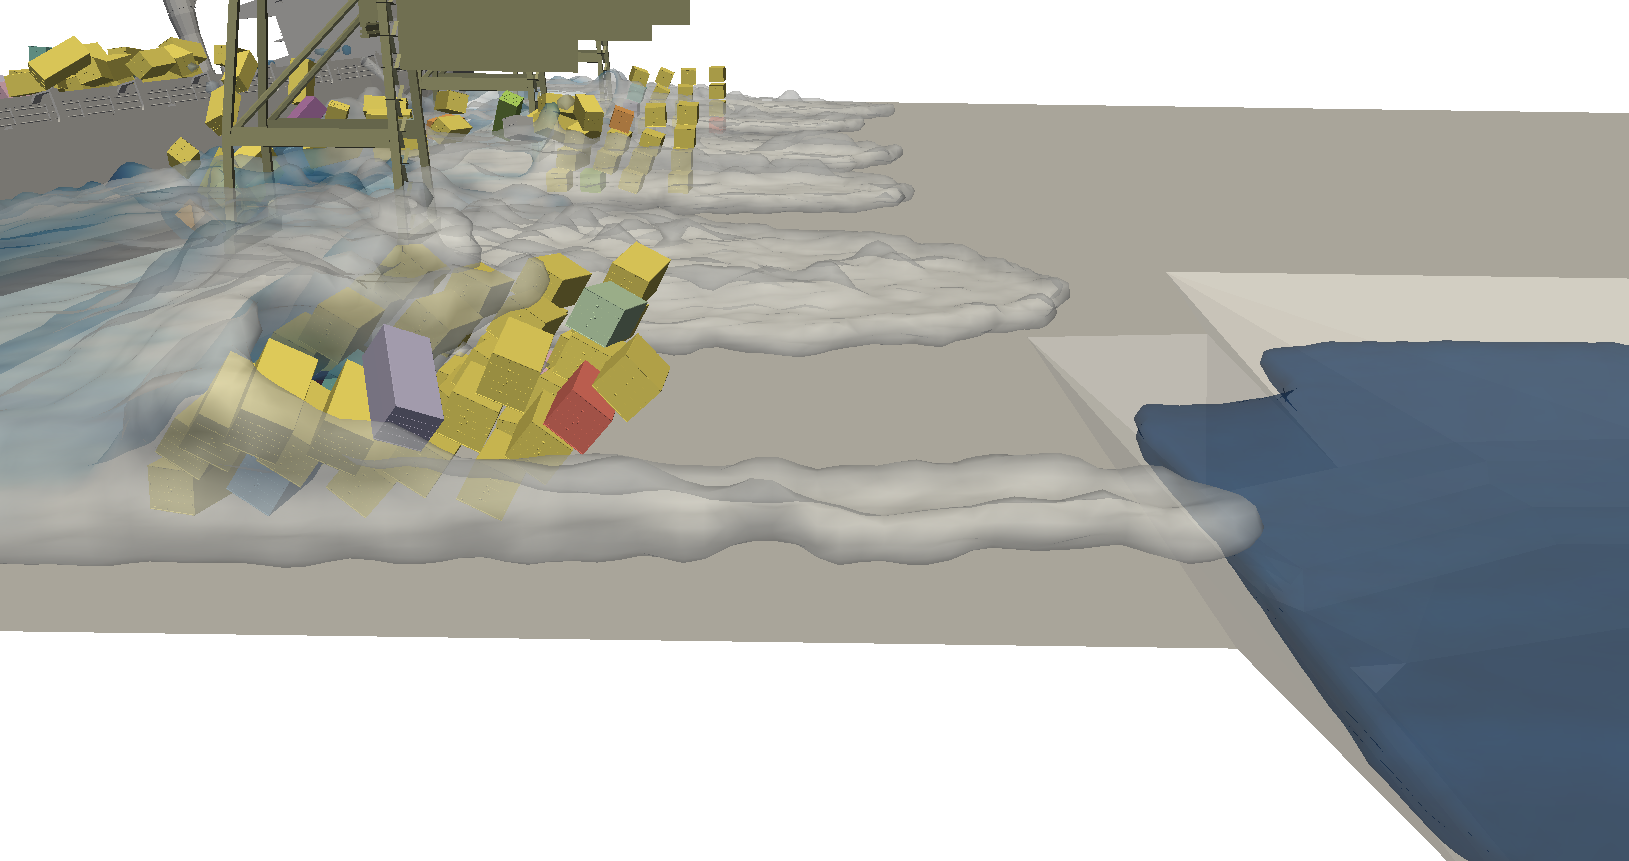
\includegraphics[width=0.95\linewidth]{Figures/6.Chapter/cont_t80} 
	\caption{Details of a set of container stacks, $t=16.0$ s.}
	\label{fig:cont_t80} 
\end{figure}
%
%
\begin{figure}[H]
	\centering
	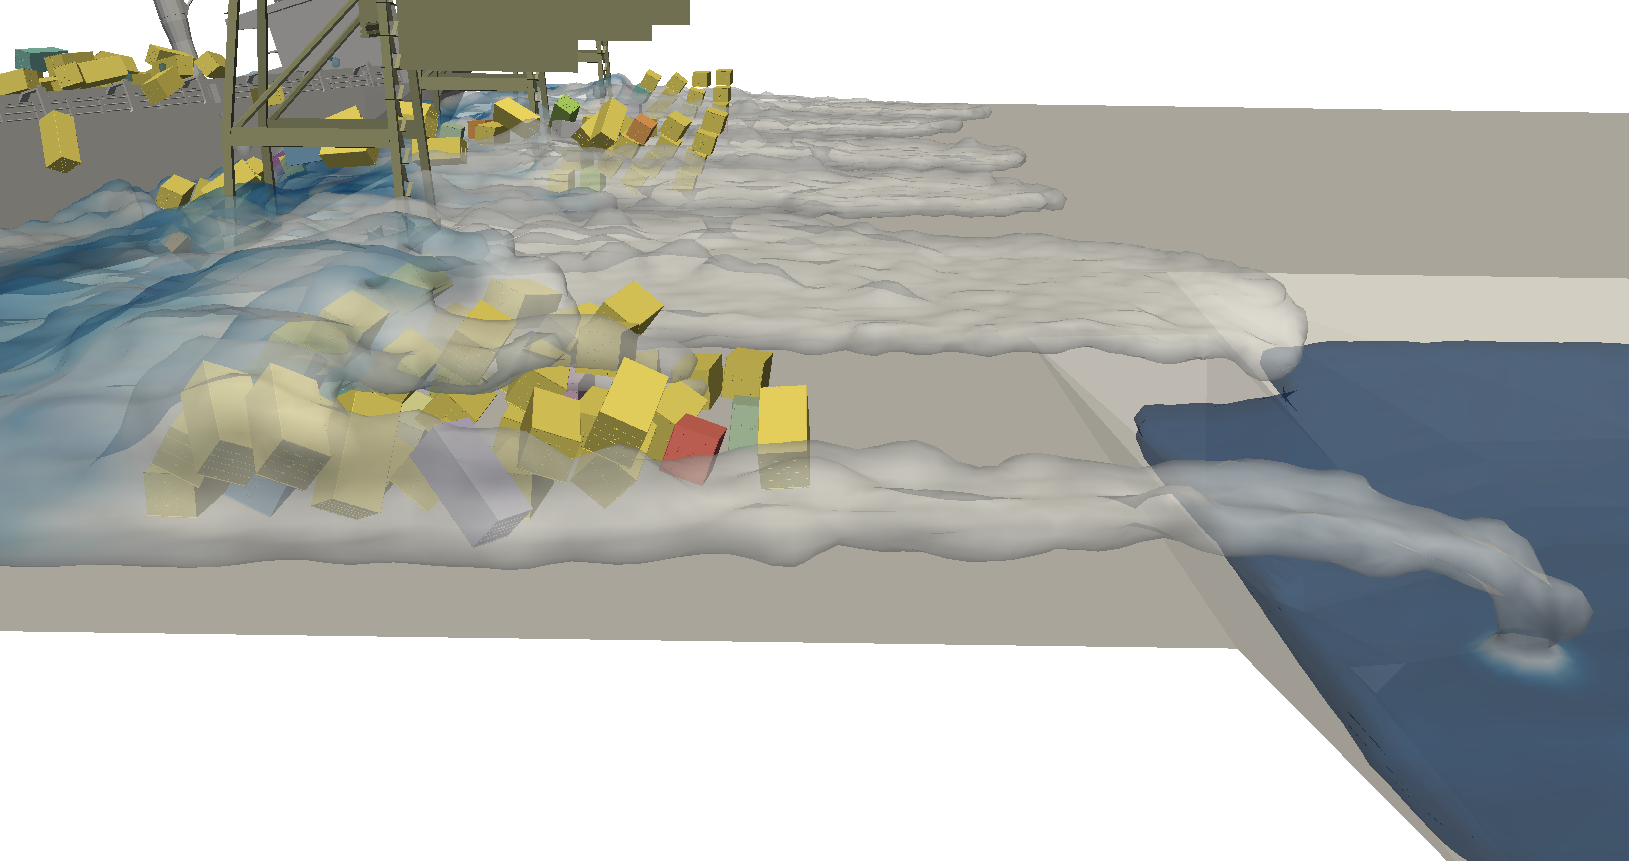
\includegraphics[width=0.95\linewidth]{Figures/6.Chapter/cont_t85} 
	\caption{Details of a set of container stacks, $t=17.0$ s.}
	\label{fig:cont_t85} 
\end{figure}
%
%
\begin{figure}[H]
	\centering
	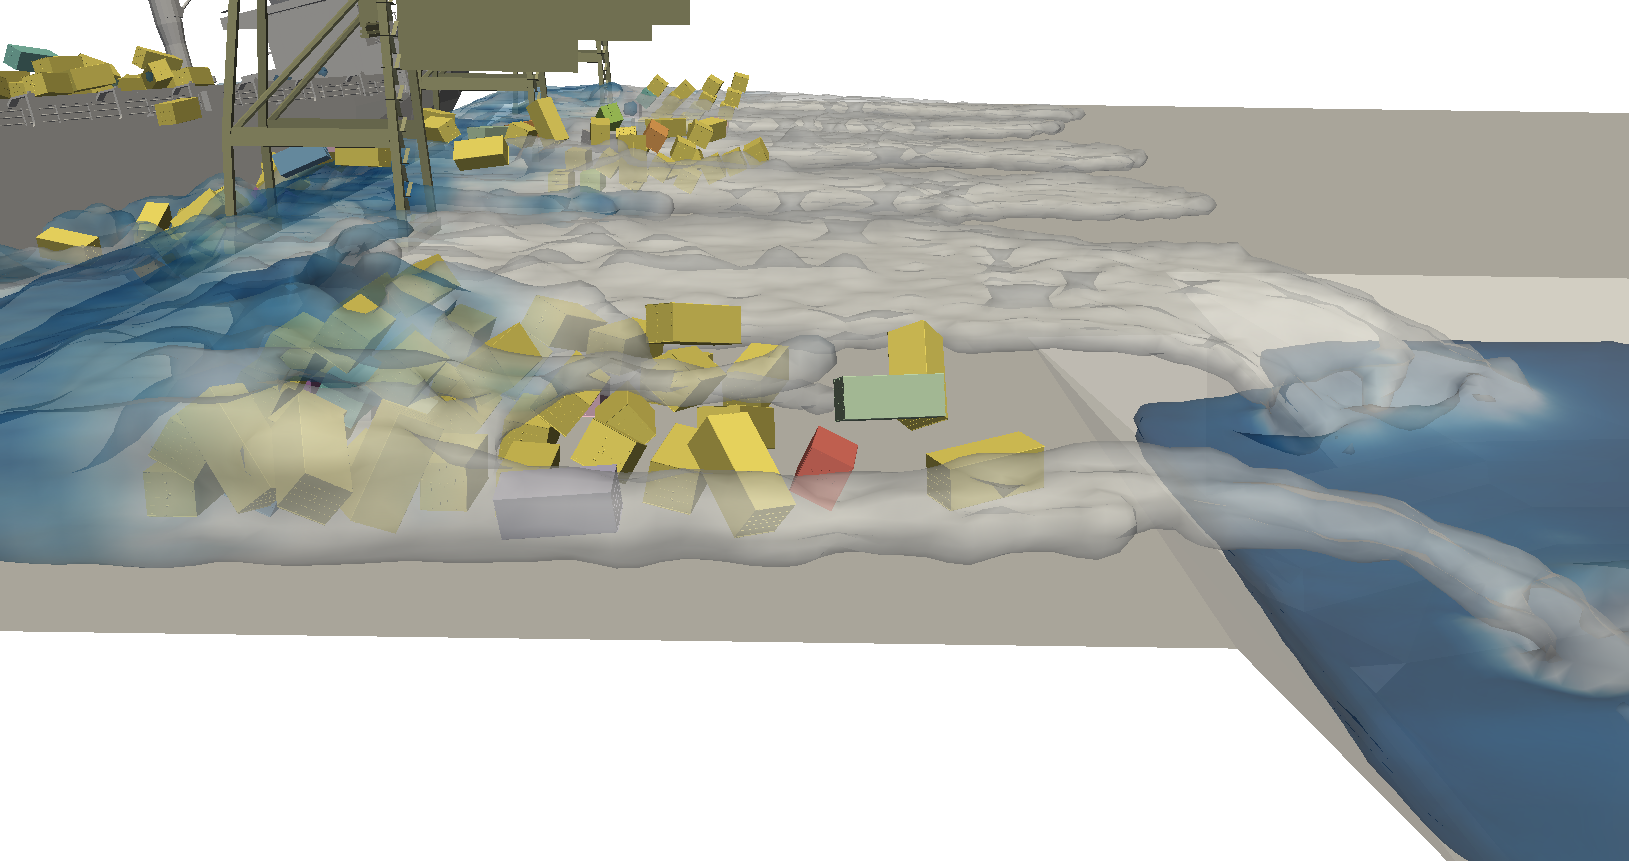
\includegraphics[width=0.95\linewidth]{Figures/6.Chapter/cont_t90} 
	\caption{Details of a set of container stacks, $t=18.0$ s.}
	\label{fig:cont_t90} 
\end{figure}
%

At $t=60.0$ s, Figure \ref{fig:cont_t300} shows the final set of the numerical solution. 
%
\begin{figure}[H]
	\centering
	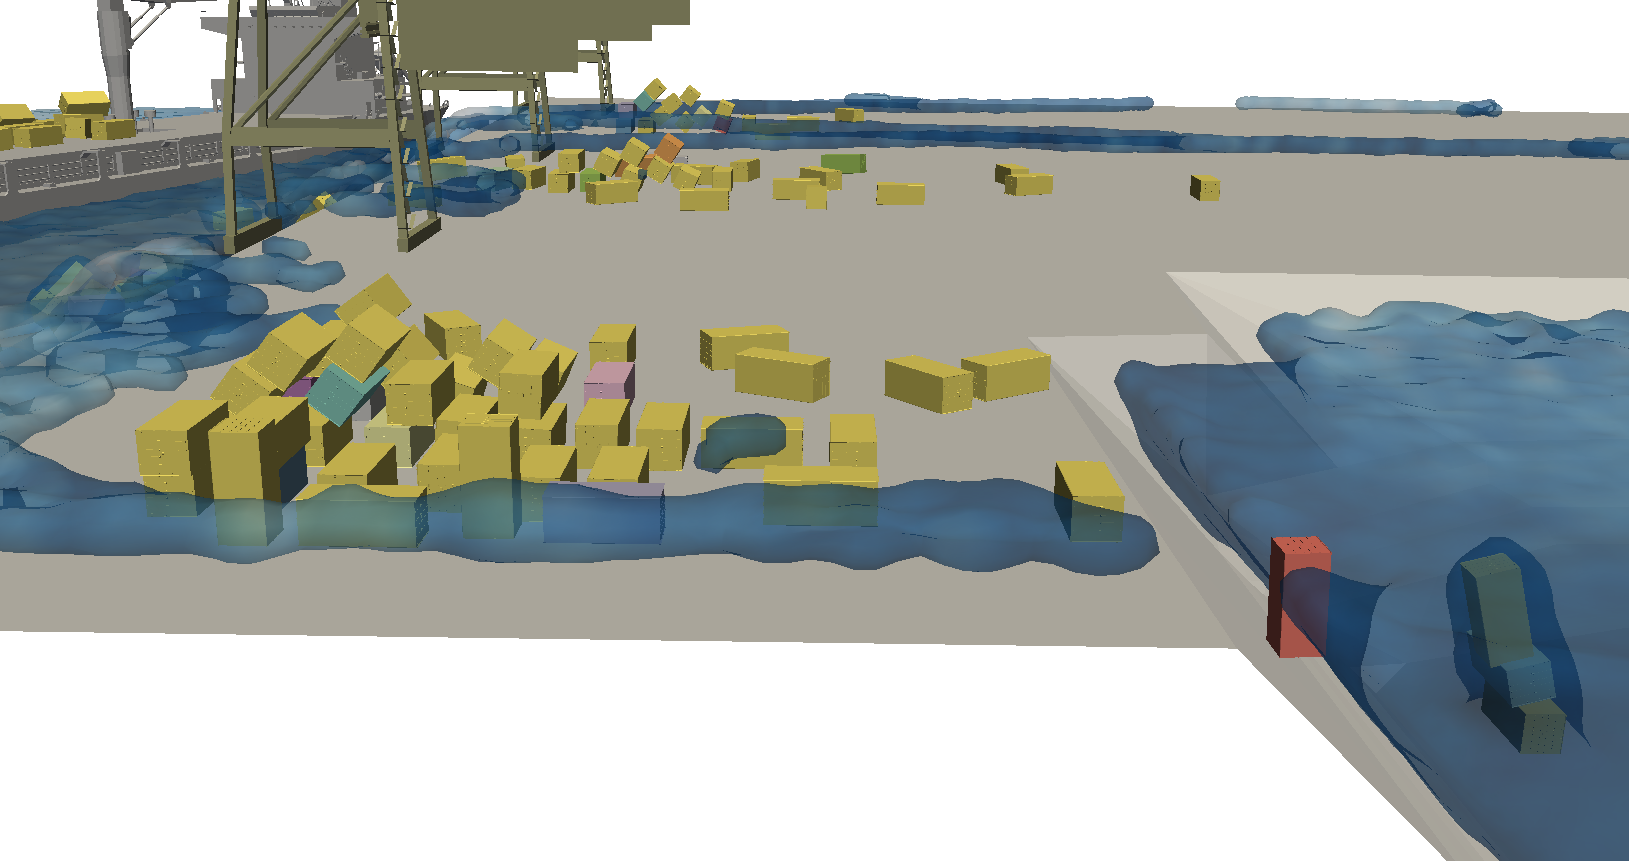
\includegraphics[width=0.95\linewidth]{Figures/6.Chapter/cont_t300} 
	\caption{Details of a set of container stacks, $t=60.0$ s.}
	\label{fig:cont_t300} 
\end{figure}
%
Some containers were projected across the structure platform but most did not incur in a significant dislocation. New equilibrium positions were achieved by the group of containers, showing the effectiveness of the contact mechanisms to provide balanced solutions even in complex configurations.

Focusing on the behavior of the ship containers aboard the ship, Figures \ref{fig:ship_t38} and \ref{fig:ship_t45} show the beginning of the instabilization as the wave passes, at $t=7.6$ s and $t=9.0$ s, respectively.
%
\begin{figure}[H]
	\centering
	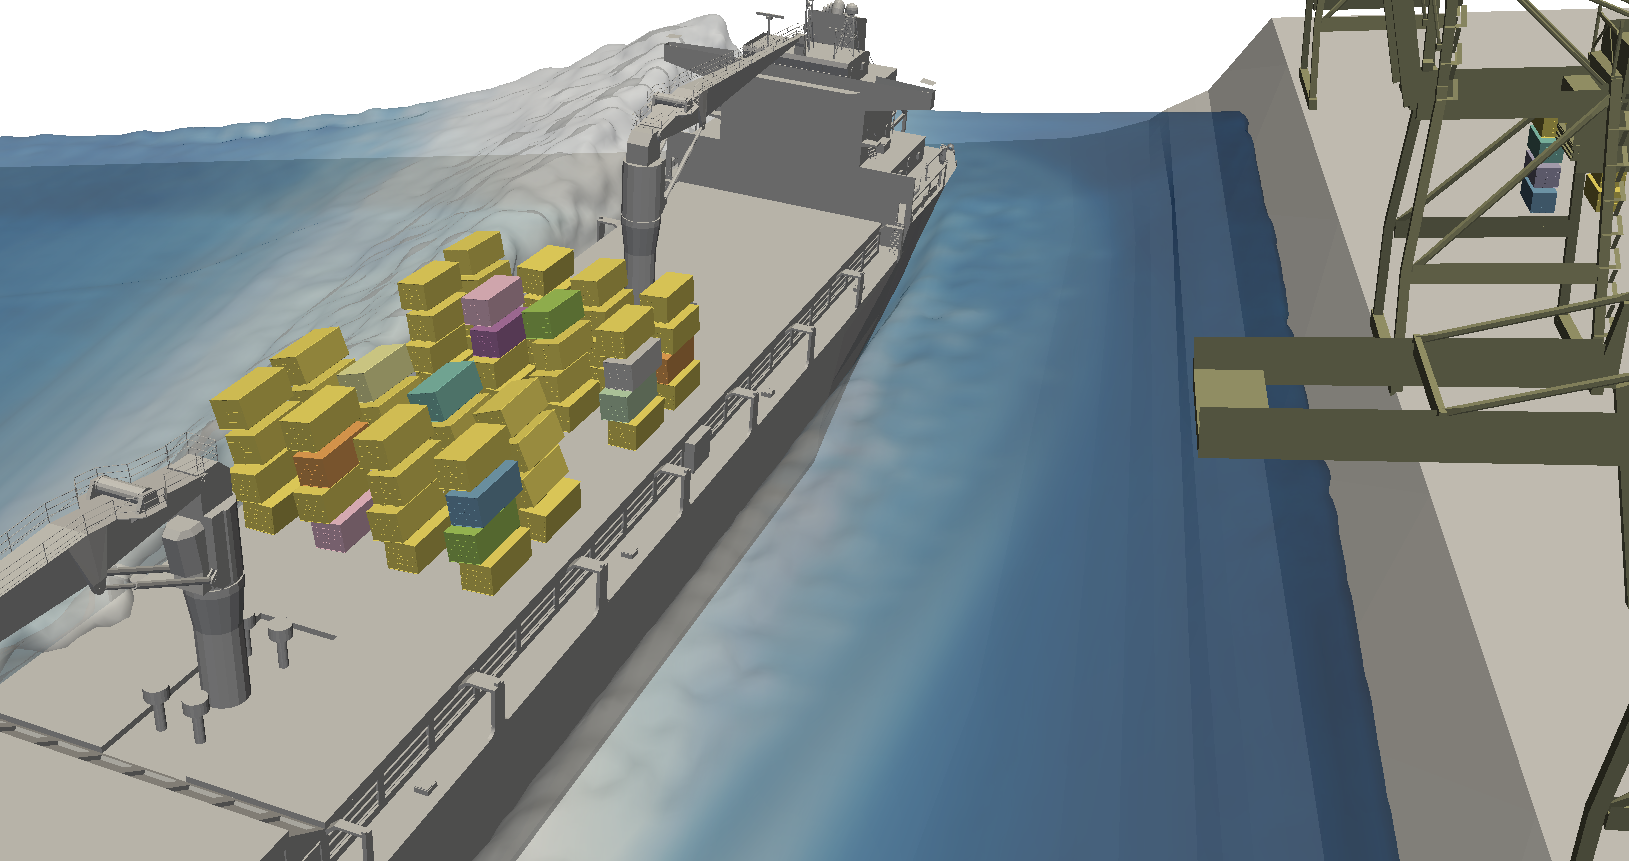
\includegraphics[width=0.95\linewidth]{Figures/6.Chapter/ship_t38} 
	\caption{Behavior of the ship-containers system, $t=7.6$ s.}
	\label{fig:ship_t38} 
\end{figure}
%
%
\begin{figure}[H]
	\centering
	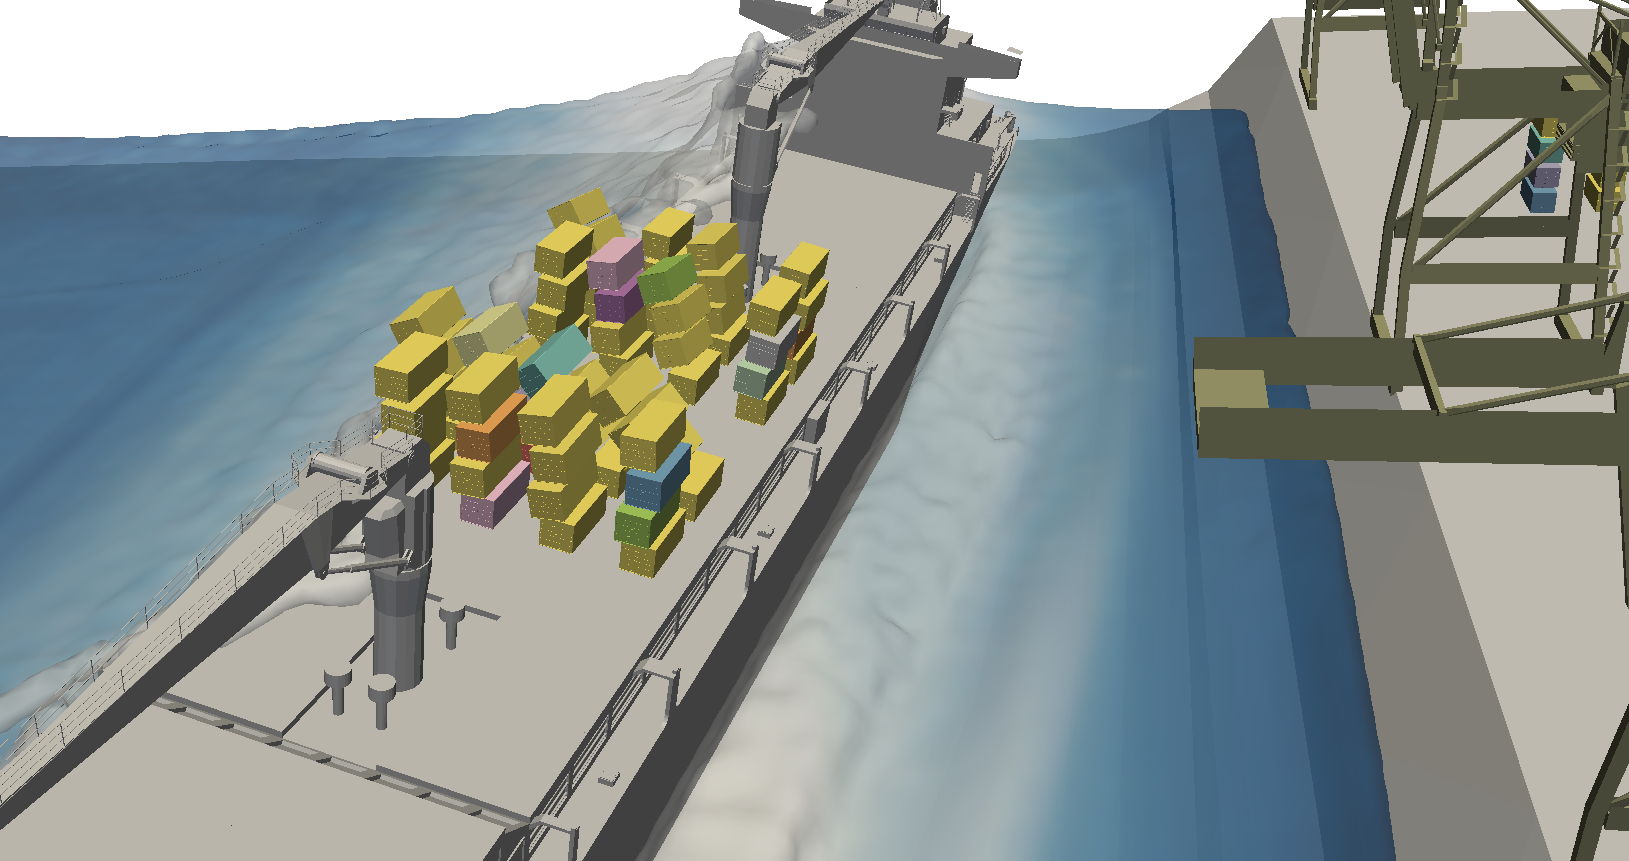
\includegraphics[width=0.95\linewidth]{Figures/6.Chapter/ship_t45} 
	\caption{Behavior of the ship-containers system, $t=9.0$ s.}
	\label{fig:ship_t45} 
\end{figure}
%

Figure \ref{fig:ship_t55} reflects the state of the system at $t=11.0$ s, were every set of containers is now in significant motion.
%
\begin{figure}[H]
	\centering
	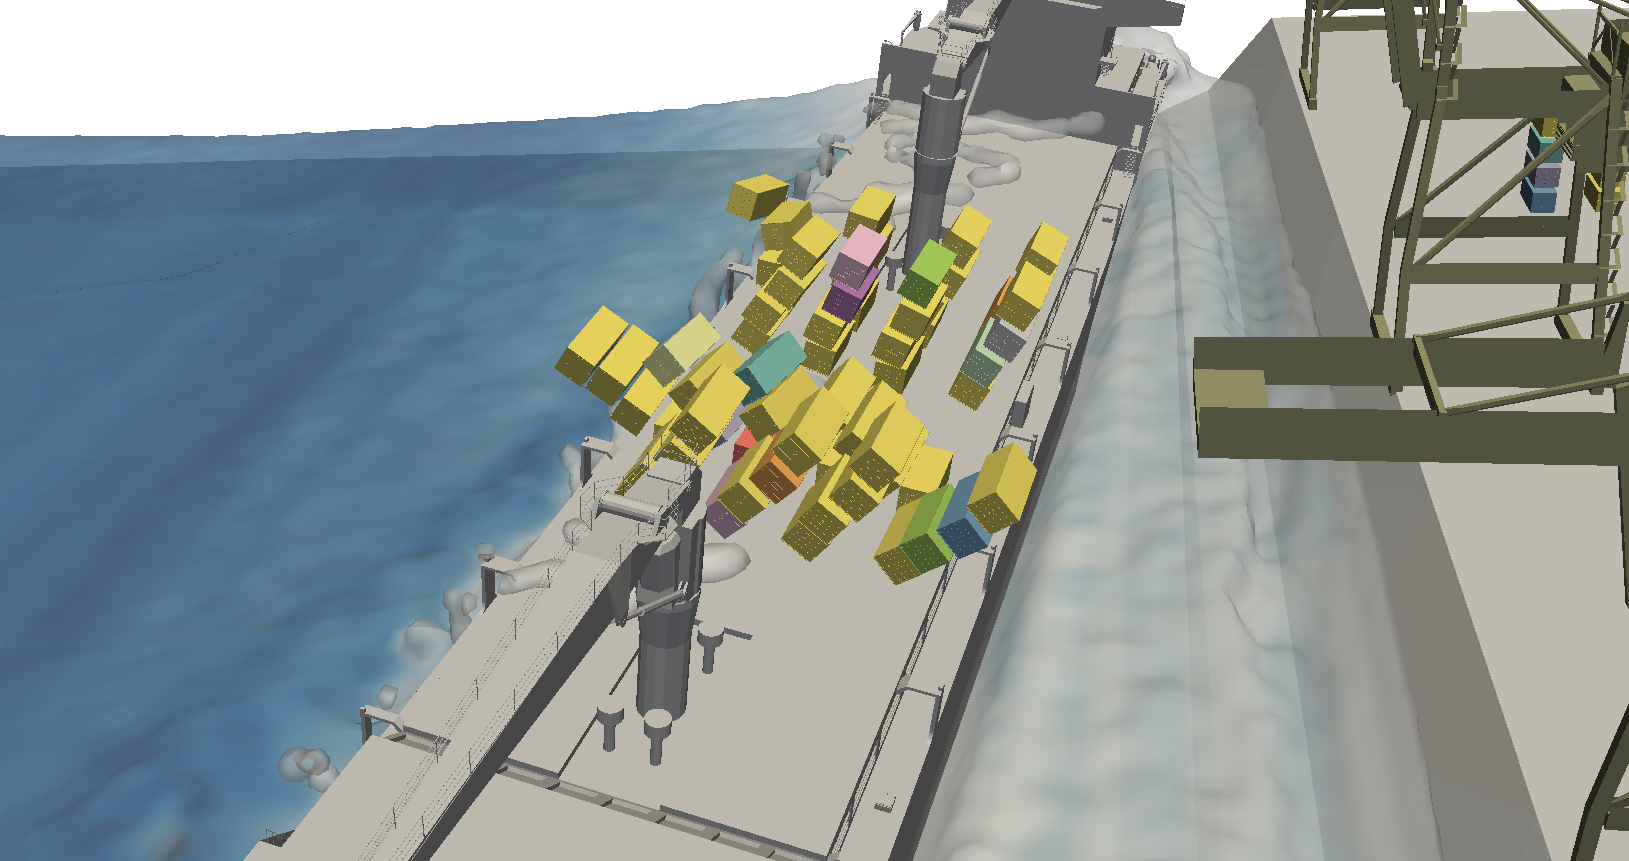
\includegraphics[width=0.95\linewidth]{Figures/6.Chapter/ship_t55} 
	\caption{Behavior of the ship-containers system, $t=11.0$ s.}
	\label{fig:ship_t55} 
\end{figure}
%

The uppermost containers are falling over the ship starboard-side, mostly due to inertia. The bottom containers, after being imprinted with the ship velocity by the friction mechanism, start sliding and falling port-side, as can be seen in Figure \ref{fig:ship_t65}. Such is due to the sudden acceleration of the ship caused by collision with the bottom and padding by the wave, now mostly between the ship and the harbor structure.
%
\begin{figure}[H]
	\centering
	\includegraphics[width=0.95\linewidth]{Figures/6.Chapter/ship_t65} 
	\caption{Behavior of the ship-containers system, $t=13.0$ s.}
	\label{fig:ship_t65} 
\end{figure}
%

At the end of the simulation a considerable number of containers were transferred inland and a small amount fell overboard and are now in the fluid. The remaining containers have a solitary motion with the ship, as can be seen in Figure \ref{fig:ship_t300}, at $t=60.0$ s.
%
\begin{figure}[H]
	\centering
	\includegraphics[width=0.95\linewidth]{Figures/6.Chapter/ship_t300} 
	\caption{Behavior of the ship-containers system, $t=60.0$ s.}
	\label{fig:ship_t300} 
\end{figure}
%


\clearpage
%%%%%%%%%%%%%%%%%%%%%%%%%%%%%%%%%%%%%%%%%%%%%%%%%%%%%%%%%%%
\section{Debris Flow}
\label{sec:debris_flow}

Debris flows are regarded as one of the most feared flow-related phenomena, due to the large destructive potential of infrastructure and danger to human lives. It is no surprise that a large body of work has been produced concerning its genesis, behavior and mitigation measures, both by fundamental phenomenological approaches reduced to analytic or simplified numerical problems and experimental campaigns. The flow characteristics ensure that complex measurements on important quantities remain difficult to perform. The inwards of a debris flow has only been accessible by analogy with simpler flows and conceptual work. Hope is therefore deposited in numerical work, to provide increasingly plausible insights into the mechanics of the flow. The amount of data amassed does not meet a reliable numerical solution, however. Existing conceptual models map poorly to a satisfactory numerical solution: the span of spacial scales involved in these flows start at the smaller energy carrying flow structures, up to the largest particles in the flow, possibly in the order of meters; the time scales range from millisecond inter-particle collisions to the duration of the flow; large deformations on the non-continuous multiphasic medium difficult any traditional approximation and the highly unsteady flow and free-surface deformations pose a challenge for state-of-the-art Finite-Volume codes, considering just single phase flows.

The application of the proposed model to a debris flow is done by reproducing an experimental campaign where debris flow mitigation measures are studied. A flume is fitted with a check-dam, intended to control the transport and deposition processes of the sediments carried downstream by debris flows. Since check-dams are considered as one of the simplest and most effective engineering measures against debris flows \citep{Zeng-2008,Remaitre-2008} they were widely applied all over the world as a short-term mitigation measure. Check dams are composed of a weir, two wings and a robust foundation, although there is a variety of other check dam solutions. Open-type check dams present a very attractive characteristic: they allow small sediment particles to pass through, while trapping larger blocks. The implemented open-type check dam is a slit dam, whose effectiveness in debris flows mitigation has been documented in the literature. 

The simulations are based on a flume described in \cite{Silva-2015}, where vertical slits with a spacing $s$, a $20\%$ slope and a recirculating mechanism are the main characteristics. The numerical flume presents fully periodic conditions, allowing for both fluid and solid phase recirculation. Two slit typologies were tested, named P1 and P2, as defined in \cite{Silva-2015}. Three spacings were tested, $s/d95 \in [1.18; 1.36; 1.49]$, as per the experiments. Figure \ref{fig:Slits} shows the dam section apparatus and defines the cross section of slits P1 and P2.

%
\begin{figure}[ht!]
	\centering
	\includegraphics[width=0.45\linewidth]{Figures/6.Chapter/Experimental_slits}
	\includegraphics[width=0.20\linewidth]{Figures/6.Chapter/p1_slits}
	\includegraphics[width=0.205\linewidth]{Figures/6.Chapter/p2_slits}
	\caption{Experimental dam configuration. Slits P1 and P2 specifications. \citep{Silva-2015}}
	\label{fig:Slits} 
\end{figure}
%

The scales of the sediment grain interactions are orders of magnitude inferior to the $d50$ of the granulometric curve. This may represent a problem for the numerical discretization, as even smaller distances need to be evaluated for the force computations (Equation \eqref{eq:normal_viscoelastic_I}), and machine precision can start to affect the computations after a large number of iterations. In order to curb such effect, the geometric scale of the numerical experiment was doubled, as 

%
\begin{equation} \label{eq:Debris_scale_I}
	\lambda_l=\frac{L_m}{L_p}=2
\end{equation}
%
where $\lambda_l$ is the geometrical scale, $L_m$ is the characteristic length of the model and $L_p$ the same length on the physical prototype. Assuming Froude similarity, the discharge scales as
%
\begin{equation} \label{eq:Debris_scale_II}
	\lambda_Q=\frac{\lambda_V}{\lambda_t}=\frac{\lambda_l^3}{\lambda_l^{1/2}}=\lambda_l^{5/2}
\end{equation}
%

It is considered that liquid and solid discharges introduced upstream are independent, i.e., it is not intended that the solid discharge corresponds to the capacity discharge for the given liquid discharge, considering the inclination, geometry and roughness of the flume. Table \ref{tab:discharges} shows the used model discharges and the corresponding prototype values.

\begin{table}[!ht]
\begin{center}
\begin{tabular}{l|ll} 
 & Prototype & Model \\
\hline
$Q_l (m^3s^{-1})$ & 0.018 & 0.1018 \\
$Q_s (m^3s^{-1})$ & 0.00033 & 0.0018 
\end{tabular}
\end{center}
\caption{Model and prototype discharges}
\label{tab:discharges}
\end{table}

To promote a correct inlet of solid material, a hopper is modeled, placed on top of the channel. It was heuristically dimensioned to ensure an average solid discharge compatible with the one presented in Table \ref{tab:discharges}. 
Solid sediment grain sizes are generated according to a random algorithm that reproduces a log-normal function, effectively approximating the granulometric curve from \cite{Silva-2015}. The grains are dispersed in the hopper and are let to achieve their natural equilibrium positions at the start of the simulation. The initial conditions generation routines allows to create entirely distinct solutions based on the same granulometric curves, hence with comparable statistical properties, effectively corresponding to different experimental runs.

The proposed parameters for the material properties, used in Equations \eqref{eq:normal_viscoelastic_I} to \eqref{eq:elastic_fric}, are summarized in Table \ref{tab:materials}.

\begin{table}[!ht]
\begin{center}
\begin{tabular}{l|l} 
$E (GNm^{-2})$ & 45 \\
\hline
$\nu (-)$ & 0.35 \\
\hline
$\mu (-)$ & 0.35 
\end{tabular}
\end{center}
\caption{Sediment mechanical characteristics}
\label{tab:materials}
\end{table}

The resolution of the model was set at $0.008 \; m$, resulting in over $1.6\times10^6$ particles. 8 parallel simulations were carried out at a time on a Nvidia K20x cluster, each taking in excess of 280 h to model the 70 s runs, due to the very demanding stability constraints on time step. An overview of the domain can be seen in Figure \ref{fig:overall}.
%
\begin{figure}[ht!]
	\centering
	\includegraphics[width=0.75\linewidth]{Figures/6.Chapter/frame4}
	\caption{Overall domain configuration.}
	\label{fig:overall} 
\end{figure}
%

The sediment trapping efficiency is accounted by measuring the solid discharges at a position sufficiently upstream and immediately downstream of the dam. The experimental procedure estimated these by measuring the volumes of the sediment that was trapped downstream of the dam and by knowing the volume placed at the inlet. Due to the recirculation of solid particles, for the analysis of the numerical solution such approach is impractical, and discharges are computed directly by analyzing the flux of solid particles crossing a given plane.

Immediately after the opening of the hopper, a substantial amount of material falls to the flume, as indicated in Figure \ref{fig:t_2}, at $t=3.0$ s.
%
\begin{figure}[ht!]
	\centering
	\includegraphics[width=0.75\linewidth]{Figures/6.Chapter/frame_II}
	\caption{P1 type slits, $t=3.0$ s}
	\label{fig:t_2} 
\end{figure}
%

As the material is carried downstream, deposition starts at the dam section. Figure \ref{fig:t_35} shows in detail a render of the solution in the dam area, at $t=8.0$ s.
%
\begin{figure}[ht!]
	\centering
	\includegraphics[width=0.75\linewidth]{Figures/6.Chapter/frame_V}
	\caption{P1 type slits, $t=8.0$ s}
	\label{fig:t_35} 
\end{figure}
%

As the material is dispensed from the hopper, the retention upstream of the dam becomes more effective. At $t=35.0$ s, the state of the solution is represented in Figure \ref{fig:t_350}. 
%
\begin{figure}[ht!]
	\centering
	\includegraphics[width=0.75\linewidth]{Figures/6.Chapter/frame_III}
	\caption{P1 type slits, $t=35.0$ s}
	\label{fig:t_350} 
\end{figure}
%

Figures \ref{fig:t_2} to \ref{fig:t_350} are rendered from a particular simulation. As the sediment particles are generated with a random arrangement as initial conditions, significant instantaneous variations occur if one compares similar runs. On average, at $t=40.0$ s the hopper is exhausted and the flow is assumed to reach equilibrium conditions close to $10$ s after that, when the last solid particle reaches the backwater of the dam. A $15$ s interval was used to count solid discharges and derive retention trapping rates. Table \ref{tab:P1tr_comp} and Figure \ref{fig:P2tr_comp} show the relationship between sediment trapping efficiency, E, and the relative spacing $s/d95$ for each tested solution. 

\begin{table}[!ht]
\begin{center}
\begin{tabular}{l|llll} 
$s/d95$ & E[-] (Exp) & E[-] (Run I)& E[-] (Run II)& E[-] (Run III)\\
\hline
1.180 & 0.900 & 0.786 & 0.802 & 0.810 
\end{tabular}
\end{center}
\caption{Sediment trapping efficiency results. P1 type slits.}
\label{tab:P1tr_comp}
\end{table}

%
%\begin{figure}[ht!]
%	\centering
%	\includegraphics[width=0.50\linewidth]{Figures/6.Chapter/P1tr}
%	\caption{Sediment trapping efficiency results. P1 type slits. Experimental ($\cdot$) Numerical ($\square$)}
%	\label{fig:P1tr_comp} 
%\end{figure}
%

%
\begin{figure}[ht!]
	\centering
	\includegraphics[width=0.50\linewidth]{Figures/6.Chapter/P2tr}
	\caption{Sediment trapping efficiency results. P2 type slits. Experimental ($\cdot$) Numerical ($\square$)}
	\label{fig:P2tr_comp} 
\end{figure}
%

The numerical results present a good comparison with the experimental data. A noticeable under prediction of the efficiency for small spacings is shown, for both slit geometries. For P2 slits the trend is accompanied with increasing spacing, but no zero efficiency is established for $s/d95=1.49$, contrasting with the experimental results. This is due to single sediment particles getting retained for long enough to affect the measurements on the numerical solution.

The differences should be explained both by discretization shortcomings and differences in the initial conditions from the experimental to numerical experiments. Besides conceptual considerations, the doubling of the geometrical dimensions to allow for more relaxed length and time scales is bound to introduce differences in the flow depth in the locus of the dam. This is because Froude similarity is not an exact hypothesis in the vicinity of the slits. This may affect the retention properties of the numerical dam, but insufficient experimental data is available to provide more insight. Another important difference is related to the initial conditions of the experimental procedure. These are not marked by a smooth, fixed bed: an approximately $5\;cm$ thick layer of sediment is deposited along the flume, also contributing to the total amount of mobile solid material if the flow is capable of mobilizing it, besides introducing considerable resistance to the flow.

The slit density, $\gamma_s$, is given by the ratio between the sum of all functional openings and the dam width, that influences water and solid discharges. Figure \ref{fig:SD_P1} shows the sediment trapping rate $E$ versus the slit density.

%
\begin{figure}[ht!]
	\centering
	\includegraphics[width=0.50\linewidth]{Figures/6.Chapter/SD_P1}
	\caption{Sediment trapping rate as a function of slit density. P1 type slits for $s/d95=1.18$. Experimental ($\cdot$) Numerical ($\square$)}
	\label{fig:SD_P1} 
\end{figure}
%

An increase in slit density appears to induce increased efficiency of the solution, enhancing deposition upstream of the slit-dam. This is in line with the findings of \cite{Wenbing-2006}. For the same discharge, the average flow velocity decreases and the local stream power decreases too, resulting in the local reduction of sediment transport capacity. This effect seems to be captured in the numerical solution, albeit with the already discussed differences.








\cleardoublepage

%\cleardoublepage
%% %%%%%%%%%%%%%%%%%%%%%%%%%%%%%%%%%%%%%%%%%%%%%%%%%%%%%%%%%%%%%%%%%%%%%%
% Dummy Chapter:
% %%%%%%%%%%%%%%%%%%%%%%%%%%%%%%%%%%%%%%%%%%%%%%%%%%%%%%%%%%%%%%%%%%%%%%

% %%%%%%%%%%%%%%%%%%%%%%%%%%%%%%%%%%%%%%%%%%%%%%%%%%%%%%%%%%%%%%%%%%%%%%
% The Introduction:
% %%%%%%%%%%%%%%%%%%%%%%%%%%%%%%%%%%%%%%%%%%%%%%%%%%%%%%%%%%%%%%%%%%%%%%
\fancychapter{Applications}
\label{cap:chapter_apps}

\textit{Fulfilling the objectives of the dissertation, fringe areas (in the sense that there is hardly any numerical tool that tackled these issues without serious simplifications) are explored in this chapter. These are intrinsically preliminary results and analysis of the solutions. There are no complete set of measurements on any of these cases and, as such, validation of the solution can not be performed directly. It is the hope of the author that the model can inspire more research on this class of topics, by presenting the first available interactive sketch on them.\\
For the sake of completeness, simulation times are included. All of the simulations were performed on a Nvidia Titan GPU from 2013.}

\section{Coastal Geomorphology}
\label{sec:coastal_geomorphology}

The Portuguese coast presents high tsunami inundation risk in comparison with other locations of the Atlantic Europe due to its close location in relation to the Azores-Gibraltar plate boundary.
The Portuguese coastline presents several high-energy sedimentary deposits\footnote{Typically associated with intense wave activity, promoting resuspension and transport of larger particles.} associated with onshore depositional activity from the AD 1755 Lisbon event, with both large and small boulders located above mean sea level and occurring between Lisbon and the central Algarve attributed to deposition by this and older tsunamis \citep{Scheffers-2005, Costa-2008}. Furthermore, the western Portuguese coast is also very exposed to Atlantic storms, and wave power associated with wind-generated waves is also very high \citep{Oliveira-2011}. 

Such characteristics make the western coast of Portugal an important study area regarding entrainment and transport of large clasts (including megaclasts) by storm or tsunami waves, a matter that has been profusely discussed in the literature in the last decade. Although the exact mechanism that originates such deposits still lacks an exact comprehension, several authors used conventional numerical solutions that simulate particle transport, sometimes with contradictory results \citep{Nandasena-2011, Kain-2012}. The biggest challenge has been the differentiation of the events (storm or tsunami), and the reconstruction of wave parameters (e.g. wave height, length, direction) responsible for the entrainment and transport of these megaclasts. Conceptual efforts have been made to distinguish between the two, with the most popular approach being \cite{Nott-2003} methodology, that attempts to differentiate the two origins in a variety of dynamic and geological environments, but disregarding local features.

A practical example of such phenomena can be observed in Praia das Ma\c{c}\~{a}s, Portugal. The location is a pocket beach encased in a high energy exposed cliffed coast. The geology consists of Cretaceous soft marls alternated with resistant limestone. A seaward sloping close to $80$ m wide stepped rock platform develops at the cliff toe. The step characteristics are controlled by practically vertical fractures and the thickness of the resistant limestone layers, typically close to $1$ m. In Figure \ref{fig:boulders_exp}, two boulders that suffered transport are identified.

%
\begin{figure}[ht!]
	\centering
	\includegraphics[width=0.85\linewidth]{Figures/6.Chapter/boulders_exp} 
	\caption{Praia das Ma\c{c}\~{a}s, Portugal. Boulder identification and orientation. \cite{Oliveira-2011}}
	\label{fig:boulders_exp} 
\end{figure}
%

Boulder B1 is $2.80\times2.0\times1.0$ m and weighs approximately 14 ton. It appears to have suffered a rotation and a small translation from the initial position. In this exploratory Section, the proposed model is applied as an inverse-problem, attempting to reproduce the dislodgement of megaclast, i.e, it is hypothesized that the pattern of deposition may be partially explained by actually modeling specific events in real geometries, attempting to recover the final observed state. 

The geometry of the problem is idealized but represents the key features of the overhanging layers related with fractures, bedding and differential erosion of sub-horizontal layers that originated block B1. In plan view, concave and convex coastline shapes are tested to assess the influence of momentum accumulation. A paddle with prescribed motion was used to generate a wave with $40\;m$ wavelength and $15\;m$ height, reproducing a large storm wave that breaks at the beach section. The lateral dimension is periodic to avoid any wall effects and the $2.84\times10^6$ particles are a result of $Dp=0.10\;m$ resolution, forcing 13 h long computations for 25 s events. The megaclast is assumed to be homogeneous limestone, with $E=4.5\times10^8 Nm^{-2}$, $\nu=0.15$ and $\mu=0.60$. Figures \ref{fig:boulders_I} to \ref{fig:boulders_IV} show the evolution of the system as the wave impacts the overhanging boulder.

%
\begin{figure}[ht!]
	\centering
	\includegraphics[width=0.42\linewidth]{Figures/6.Chapter/concave_105} 
	\includegraphics[width=0.42\linewidth]{Figures/6.Chapter/convex_105}
	%\includegraphics[width=0.13\linewidth]{Figures/6.Chapter/label} 
	\caption{Concave and convex geometries, $t=10.5$ s.}
	\label{fig:boulders_I} 
\end{figure}
%

%
\begin{figure}[ht!]
	\centering
	\includegraphics[width=0.42\linewidth]{Figures/6.Chapter/concave_115} 
	\includegraphics[width=0.42\linewidth]{Figures/6.Chapter/convex_115} 
	%\includegraphics[width=0.13\linewidth]{Figures/6.Chapter/label} 
	\caption{Concave and convex geometries, $t=11.5$ s.}
	\label{fig:boulders_II} 
\end{figure}
%

%
\begin{figure}[ht!]
	\centering
	\includegraphics[width=0.42\linewidth]{Figures/6.Chapter/concave_120} 
	\includegraphics[width=0.42\linewidth]{Figures/6.Chapter/convex_120} 
	%\includegraphics[width=0.13\linewidth]{Figures/6.Chapter/label} 
	\caption{Concave and convex geometries, $t=12.0$ s.}
	\label{fig:boulders_III} 
\end{figure}
%

%
\begin{figure}[ht!]
	\centering
	\includegraphics[width=0.42\linewidth]{Figures/6.Chapter/concave_130} 
	\includegraphics[width=0.42\linewidth]{Figures/6.Chapter/convex_130} 
	%\includegraphics[width=0.13\linewidth]{Figures/6.Chapter/label} 
	\caption{Concave and convex geometries, $t=13.0$ s.}
	\label{fig:boulders_IV} 
\end{figure}
%

Differences in concave to convex geometries are within expectation: momentum seems to be concentrated in the concave case, as the megaclast rotates faster (Figure \ref{fig:boulders_III}) and is transported around $1$ m further comparing to the convex case. 

Another fundamental aspect of the phenomenon is overhanging versus supported geometry. Two contact forces are responsible for the dislodgement of the boulders: pressure and momentum flux. The main working force is the momentum flux, but the work of both for the boulder movement is proportional to the area exposed. Figures \ref{fig:boulders_V} and \ref{fig:boulders_VI} show the pressure field on the impact locus. 

%
\begin{figure}[ht!]
	\centering
	\includegraphics[width=0.48\linewidth]{Figures/6.Chapter/2D_press_norm_I} 
	\includegraphics[width=0.48\linewidth]{Figures/6.Chapter/2D_press_norm_II}
	\caption{Concave geometry. Vertical plane over domain axis. Overhanging case. Left-$t=10.9$ s, right-$t=11.5$ s.}
	\label{fig:boulders_V} 
\end{figure}
%

%
\begin{figure}[ht!]
	\centering
	\includegraphics[width=0.48\linewidth]{Figures/6.Chapter/2D_press_flat}
	\caption{Concave geometry. Vertical plane over domain axis. Supported case. $t=11.5$ s.}
	\label{fig:boulders_VI} 
\end{figure}
%

As expected, a significant pressure build-up occurs in the impact locus. The cavity in the overhanging configuration allows the contact forces to produce work on the boulder, in contrast with the supported case.

The local (micro to meso-scale) geomorphological conditions in rocky coastal contexts strongly control the capability of waves to entrain and transport large particles upward and inland. The flow modulation induced by these features is not adequately addressed by conventional numerical solutions and requires the application of models capable of explicitly resolving the momentum transfer between phases and take into account complex geometrical considerations.





%%%%%%%%%%%%%%%%%%%%%%%%%%%%%%%%%%%%%%%%%%%%%%%%%%%%%%%%%%%
\section{Sines Port}
\label{sec:sines}

The Sines Container Terminal, called Terminal XXI, is a major infrastructure in the Portuguese coast, currently capable of handling 1,100,000 TEU, with plans of extending up to 1,700,000 TEU. As mentioned in Section \ref{sec:coastal_geomorphology} Portugal's Atlantic coast, especially southwards of Lisbon, is subject to a non negligible risk of tsunami waves caused by seismic events that occur offshore. These results show the influence of a wave in stacked containers and other obstacles in a reduced subsection of the quay, detailed in Figure \ref{fig:sines_map}.

%
\begin{figure}[ht!]
	\centering
	\includegraphics[width=0.80\linewidth]{Figures/6.Chapter/map_sines_domain} 
	\caption{Aerial view of the Terminal XXI of the Sines Port. Red square indicates the computational domain.}
	\label{fig:sines_map} 
\end{figure}
%

The section of the harbor is partially protected by a breakwater to the east, neglected in this case to simplify the behavior of the wave on the area of interest. The chosen domain originates an excess of $12\times10^6$ particles, for a $Dp=0.5$ m, resulting in a 57 h long computation for the 60 s event. The type of wave to be generated must observe some limitations, since the wavelength must be less than the domain extent, to avoid issues at the boundaries. As stated, the breakwater is disregarded, not having any influence in the simulated wave. The equations used to generate the solitary wave were \citep{Dean-Dalrymple-1991}

%
\begin{equation} \label{eq:solitary_wave}
	V=\sqrt{\frac{4D^3}{3H}}; \;\;\; \eta(x')=\frac{D}{\cosh^2\left(\frac{x'}{V}\right)} ; \;\;\; v(x')=\eta(x')\sqrt{\frac{-g}{D}}
\end{equation}
%
where $D$ is the fluid depth, $H$ is the maximum wave height, $\eta=D+H$ and $x'$ is a coordinate normal to the wave axis measured from the wave apex. Propagating a wave from a synthetic tsunami generates a wave height of $15$ m, corresponding, according to equations \eqref{eq:solitary_wave} to a top velocity of about $5.6\;\text{ms}^{-1}$ and wavelength of approximately $130$ m, against the expected several hundreds of an actual tsunami \cite{mavbaptista-2011}. The initial conditions of the system can be seen in Figure \ref{fig:sines_ini_cond}.

%
\begin{figure}[ht!]
	\centering
	\includegraphics[width=0.95\linewidth]{Figures/6.Chapter/sines_ini_cond_II} 
	\caption{Initial conditions of the system.}
	\label{fig:sines_ini_cond} 
\end{figure}
%

The direction of the wave is normal to the quay wall structure. A cargo ship is placed in the domain, as well as a total of 143 ship containers, 64 of which on the ship. The ship has a density of $\rho=0.3\rho_{w}$ and the center of gravity was made to coincide with that of the actual ship. The geometry consists of the actual 3D scan of a ship hull, and was discretized as hollow, since no information on the internal structure of the ship is available and it would result in the most accurate inertia tensor. The ship containers are assumed half-full and as such with a $\rho=2.5\rho_{w}$ density. Each individual body has 6 degrees of freedom, no restrictions are applied, and are made of steel. The gantry cranes are also made of steel but are represented as fixed boundaries and the terrain was considered limestone. Table \ref{tab:material_props_sines} details the parameters used in the simulations. The \emph{CFL} constant was used as $C=0.2$, artificial viscosity with $\alpha=0.05$ and $h=\sqrt{3Dp^2}$.

%
\begin{table}[h]
\centering
\begin{tabular}{l|l|llll}
 & Material & $E\;[Nm^{-2}]$ & $\nu_p\;[-]$  & $e\;[-]$ & $\mu_f\;[-]$\\ \hline
Containers/Gantry cranes/Ship & Steel & $200\times10^9$ & $0.30$ & $0.85$ & $0.55$ \\
Terrain & Limestone & $4.5\times10^9$ & $0.15$ & $0.80$ & $0.60$
\end{tabular}
\caption{Young modulus, Poisson coefficient, restitution coefficient and friction coefficient used in the simulations.}
\label{tab:material_props_sines}
\end{table}
%

The wave travels approximately $7$ s until it hits the ship. The large acceleration immediately causes the instabilization of the most forward container stacks. Figure \ref{fig:sines_t38} represents the beginning of the ship motion and one can notice the beginning of the instabilization of the containers on the port-side.
\begin{figure}[H]
	\centering
	\includegraphics[width=0.95\linewidth]{Figures/6.Chapter/sines_t38_II} 
	\caption{General view of the application case, $t=7.6$ s.}
	\label{fig:sines_t38} 
\end{figure}
%

Figure \ref{fig:sines_t60}, at $t=12.0$ s, shows the container motion after the wave passage. 
\begin{figure}[H]
	\centering
	\includegraphics[width=0.95\linewidth]{Figures/6.Chapter/sines_t60_II} 
	\caption{General view of the application case, $t=12.0$ s.}
	\label{fig:sines_t60} 
\end{figure}
%

Figures \ref{fig:sines_t70} and \ref{fig:sines_t90}, at $t=14.0$ s and $t=18.0$ s, respectively, demonstrate the wave overtopping the quay and deforming at the base of the gantry cranes and the container stacks. 
\begin{figure}[H]
	\centering
	\includegraphics[width=0.95\linewidth]{Figures/6.Chapter/sines_t70_II} 
	\caption{General view of the application case, $t=14.0$ s.}
	\label{fig:sines_t70} 
\end{figure}
%
%
\begin{figure}[H]
	\centering
	\includegraphics[width=0.95\linewidth]{Figures/6.Chapter/sines_t90_II} 
	\caption{General view of the application case, $t=18.0$ s.}
	\label{fig:sines_t90} 
\end{figure}
%
Instabilization of the piles is evident, with complex contact events being treated with no aberrant results. Containers initially aboard the ship are now in the water, most of them between the ship hull and the harbor structure.

Figure \ref{fig:sines_t300}, at $t=60.0$ s, show the state of the system at the end of simulated time.
\begin{figure}[H]
	\centering
	\includegraphics[width=0.95\linewidth]{Figures/6.Chapter/sines_t300_II} 
	\caption{General view of the application case, $t=60.0$ s.}
	\label{fig:sines_t300} 
\end{figure}
%
Some containers were dragged a considerable length, over $100\times$ its own characteristic dimensions. Large piles of containers can be seen, formed after the initial configurations were perturbed, since the wave did not have enough momentum to transport all the containers.

With a more detailed perspective over a set of containers, Figure \ref{fig:cont_t70}, at $t=14.0$ s, shows the instant immediately after wave impact. 
%
\begin{figure}[H]
	\centering
	\includegraphics[width=0.95\linewidth]{Figures/6.Chapter/cont_t70} 
	\caption{Details of a set of container stacks, $t=14.0$ s.}
	\label{fig:cont_t70} 
\end{figure}
% 

Figures \ref{fig:cont_t80},\ref{fig:cont_t85} and \ref{fig:cont_t90} show the collapse of the set of containers due to the impact of the wave. Little motion of the containers is due to sustained transport, most of the momentum arises from the potential energy in the vertical pile and short contact forces due to the collisions. 
%
\begin{figure}[H]
	\centering
	\includegraphics[width=0.95\linewidth]{Figures/6.Chapter/cont_t80} 
	\caption{Details of a set of container stacks, $t=16.0$ s.}
	\label{fig:cont_t80} 
\end{figure}
%
%
\begin{figure}[H]
	\centering
	\includegraphics[width=0.95\linewidth]{Figures/6.Chapter/cont_t85} 
	\caption{Details of a set of container stacks, $t=17.0$ s.}
	\label{fig:cont_t85} 
\end{figure}
%
%
\begin{figure}[H]
	\centering
	\includegraphics[width=0.95\linewidth]{Figures/6.Chapter/cont_t90} 
	\caption{Details of a set of container stacks, $t=18.0$ s.}
	\label{fig:cont_t90} 
\end{figure}
%

At $t=60.0$ s, Figure \ref{fig:cont_t300} shows the final set of the numerical solution. 
%
\begin{figure}[H]
	\centering
	\includegraphics[width=0.95\linewidth]{Figures/6.Chapter/cont_t300} 
	\caption{Details of a set of container stacks, $t=60.0$ s.}
	\label{fig:cont_t300} 
\end{figure}
%
Some containers were projected across the structure platform but most did not incur in a significant dislocation. New equilibrium positions were achieved by the group of containers, showing the effectiveness of the contact mechanisms to provide balanced solutions even in complex configurations.

Focusing on the behavior of the ship containers aboard the ship, Figures \ref{fig:ship_t38} and \ref{fig:ship_t45} show the beginning of the instabilization as the wave passes, at $t=7.6$ s and $t=9.0$ s, respectively.
%
\begin{figure}[H]
	\centering
	\includegraphics[width=0.95\linewidth]{Figures/6.Chapter/ship_t38} 
	\caption{Behavior of the ship-containers system, $t=7.6$ s.}
	\label{fig:ship_t38} 
\end{figure}
%
%
\begin{figure}[H]
	\centering
	\includegraphics[width=0.95\linewidth]{Figures/6.Chapter/ship_t45} 
	\caption{Behavior of the ship-containers system, $t=9.0$ s.}
	\label{fig:ship_t45} 
\end{figure}
%

Figure \ref{fig:ship_t55} reflects the state of the system at $t=11.0$ s, were every set of containers is now in significant motion.
%
\begin{figure}[H]
	\centering
	\includegraphics[width=0.95\linewidth]{Figures/6.Chapter/ship_t55} 
	\caption{Behavior of the ship-containers system, $t=11.0$ s.}
	\label{fig:ship_t55} 
\end{figure}
%

The uppermost containers are falling over the ship starboard-side, mostly due to inertia. The bottom containers, after being imprinted with the ship velocity by the friction mechanism, start sliding and falling port-side, as can be seen in Figure \ref{fig:ship_t65}. Such is due to the sudden acceleration of the ship caused by collision with the bottom and padding by the wave, now mostly between the ship and the harbor structure.
%
\begin{figure}[H]
	\centering
	\includegraphics[width=0.95\linewidth]{Figures/6.Chapter/ship_t65} 
	\caption{Behavior of the ship-containers system, $t=13.0$ s.}
	\label{fig:ship_t65} 
\end{figure}
%

At the end of the simulation a considerable number of containers were transferred inland and a small amount fell overboard and are now in the fluid. The remaining containers have a solitary motion with the ship, as can be seen in Figure \ref{fig:ship_t300}, at $t=60.0$ s.
%
\begin{figure}[H]
	\centering
	\includegraphics[width=0.95\linewidth]{Figures/6.Chapter/ship_t300} 
	\caption{Behavior of the ship-containers system, $t=60.0$ s.}
	\label{fig:ship_t300} 
\end{figure}
%


\clearpage
%%%%%%%%%%%%%%%%%%%%%%%%%%%%%%%%%%%%%%%%%%%%%%%%%%%%%%%%%%%
\section{Debris Flow}
\label{sec:debris_flow}

Debris flows are regarded as one of the most feared flow-related phenomena, due to the large destructive potential of infrastructure and danger to human lives. It is no surprise that a large body of work has been produced concerning its genesis, behavior and mitigation measures, both by fundamental phenomenological approaches reduced to analytic or simplified numerical problems and experimental campaigns. The flow characteristics ensure that complex measurements on important quantities remain difficult to perform. The inwards of a debris flow has only been accessible by analogy with simpler flows and conceptual work. Hope is therefore deposited in numerical work, to provide increasingly plausible insights into the mechanics of the flow. The amount of data amassed does not meet a reliable numerical solution, however. Existing conceptual models map poorly to a satisfactory numerical solution: the span of spacial scales involved in these flows start at the smaller energy carrying flow structures, up to the largest particles in the flow, possibly in the order of meters; the time scales range from millisecond inter-particle collisions to the duration of the flow; large deformations on the non-continuous multiphasic medium difficult any traditional approximation and the highly unsteady flow and free-surface deformations pose a challenge for state-of-the-art Finite-Volume codes, considering just single phase flows.

The application of the proposed model to a debris flow is done by reproducing an experimental campaign where debris flow mitigation measures are studied. A flume is fitted with a check-dam, intended to control the transport and deposition processes of the sediments carried downstream by debris flows. Since check-dams are considered as one of the simplest and most effective engineering measures against debris flows \citep{Zeng-2008,Remaitre-2008} they were widely applied all over the world as a short-term mitigation measure. Check dams are composed of a weir, two wings and a robust foundation, although there is a variety of other check dam solutions. Open-type check dams present a very attractive characteristic: they allow small sediment particles to pass through, while trapping larger blocks. The implemented open-type check dam is a slit dam, whose effectiveness in debris flows mitigation has been documented in the literature. 

The simulations are based on a flume described in \cite{Silva-2015}, where vertical slits with a spacing $s$, a $20\%$ slope and a recirculating mechanism are the main characteristics. The numerical flume presents fully periodic conditions, allowing for both fluid and solid phase recirculation. Two slit typologies were tested, named P1 and P2, as defined in \cite{Silva-2015}. Three spacings were tested, $s/d95 \in [1.18; 1.36; 1.49]$, as per the experiments. Figure \ref{fig:Slits} shows the dam section apparatus and defines the cross section of slits P1 and P2.

%
\begin{figure}[ht!]
	\centering
	\includegraphics[width=0.45\linewidth]{Figures/6.Chapter/Experimental_slits}
	\includegraphics[width=0.20\linewidth]{Figures/6.Chapter/p1_slits}
	\includegraphics[width=0.205\linewidth]{Figures/6.Chapter/p2_slits}
	\caption{Experimental dam configuration. Slits P1 and P2 specifications. \citep{Silva-2015}}
	\label{fig:Slits} 
\end{figure}
%

The scales of the sediment grain interactions are orders of magnitude inferior to the $d50$ of the granulometric curve. This may represent a problem for the numerical discretization, as even smaller distances need to be evaluated for the force computations (Equation \eqref{eq:normal_viscoelastic_I}), and machine precision can start to affect the computations after a large number of iterations. In order to curb such effect, the geometric scale of the numerical experiment was doubled, as 

%
\begin{equation} \label{eq:Debris_scale_I}
	\lambda_l=\frac{L_m}{L_p}=2
\end{equation}
%
where $\lambda_l$ is the geometrical scale, $L_m$ is the characteristic length of the model and $L_p$ the same length on the physical prototype. Assuming Froude similarity, the discharge scales as
%
\begin{equation} \label{eq:Debris_scale_II}
	\lambda_Q=\frac{\lambda_V}{\lambda_t}=\frac{\lambda_l^3}{\lambda_l^{1/2}}=\lambda_l^{5/2}
\end{equation}
%

It is considered that liquid and solid discharges introduced upstream are independent, i.e., it is not intended that the solid discharge corresponds to the capacity discharge for the given liquid discharge, considering the inclination, geometry and roughness of the flume. Table \ref{tab:discharges} shows the used model discharges and the corresponding prototype values.

\begin{table}[!ht]
\begin{center}
\begin{tabular}{l|ll} 
 & Prototype & Model \\
\hline
$Q_l (m^3s^{-1})$ & 0.018 & 0.1018 \\
$Q_s (m^3s^{-1})$ & 0.00033 & 0.0018 
\end{tabular}
\end{center}
\caption{Model and prototype discharges}
\label{tab:discharges}
\end{table}

To promote a correct inlet of solid material, a hopper is modeled, placed on top of the channel. It was heuristically dimensioned to ensure an average solid discharge compatible with the one presented in Table \ref{tab:discharges}. 
Solid sediment grain sizes are generated according to a random algorithm that reproduces a log-normal function, effectively approximating the granulometric curve from \cite{Silva-2015}. The grains are dispersed in the hopper and are let to achieve their natural equilibrium positions at the start of the simulation. The initial conditions generation routines allows to create entirely distinct solutions based on the same granulometric curves, hence with comparable statistical properties, effectively corresponding to different experimental runs.

The proposed parameters for the material properties, used in Equations \eqref{eq:normal_viscoelastic_I} to \eqref{eq:elastic_fric}, are summarized in Table \ref{tab:materials}.

\begin{table}[!ht]
\begin{center}
\begin{tabular}{l|l} 
$E (GNm^{-2})$ & 45 \\
\hline
$\nu (-)$ & 0.35 \\
\hline
$\mu (-)$ & 0.35 
\end{tabular}
\end{center}
\caption{Sediment mechanical characteristics}
\label{tab:materials}
\end{table}

The resolution of the model was set at $0.008 \; m$, resulting in over $1.6\times10^6$ particles. 8 parallel simulations were carried out at a time on a Nvidia K20x cluster, each taking in excess of 280 h to model the 70 s runs, due to the very demanding stability constraints on time step. An overview of the domain can be seen in Figure \ref{fig:overall}.
%
\begin{figure}[ht!]
	\centering
	\includegraphics[width=0.75\linewidth]{Figures/6.Chapter/frame4}
	\caption{Overall domain configuration.}
	\label{fig:overall} 
\end{figure}
%

The sediment trapping efficiency is accounted by measuring the solid discharges at a position sufficiently upstream and immediately downstream of the dam. The experimental procedure estimated these by measuring the volumes of the sediment that was trapped downstream of the dam and by knowing the volume placed at the inlet. Due to the recirculation of solid particles, for the analysis of the numerical solution such approach is impractical, and discharges are computed directly by analyzing the flux of solid particles crossing a given plane.

Immediately after the opening of the hopper, a substantial amount of material falls to the flume, as indicated in Figure \ref{fig:t_2}, at $t=3.0$ s.
%
\begin{figure}[ht!]
	\centering
	\includegraphics[width=0.75\linewidth]{Figures/6.Chapter/frame_II}
	\caption{P1 type slits, $t=3.0$ s}
	\label{fig:t_2} 
\end{figure}
%

As the material is carried downstream, deposition starts at the dam section. Figure \ref{fig:t_35} shows in detail a render of the solution in the dam area, at $t=8.0$ s.
%
\begin{figure}[ht!]
	\centering
	\includegraphics[width=0.75\linewidth]{Figures/6.Chapter/frame_V}
	\caption{P1 type slits, $t=8.0$ s}
	\label{fig:t_35} 
\end{figure}
%

As the material is dispensed from the hopper, the retention upstream of the dam becomes more effective. At $t=35.0$ s, the state of the solution is represented in Figure \ref{fig:t_350}. 
%
\begin{figure}[ht!]
	\centering
	\includegraphics[width=0.75\linewidth]{Figures/6.Chapter/frame_III}
	\caption{P1 type slits, $t=35.0$ s}
	\label{fig:t_350} 
\end{figure}
%

Figures \ref{fig:t_2} to \ref{fig:t_350} are rendered from a particular simulation. As the sediment particles are generated with a random arrangement as initial conditions, significant instantaneous variations occur if one compares similar runs. On average, at $t=40.0$ s the hopper is exhausted and the flow is assumed to reach equilibrium conditions close to $10$ s after that, when the last solid particle reaches the backwater of the dam. A $15$ s interval was used to count solid discharges and derive retention trapping rates. Table \ref{tab:P1tr_comp} and Figure \ref{fig:P2tr_comp} show the relationship between sediment trapping efficiency, E, and the relative spacing $s/d95$ for each tested solution. 

\begin{table}[!ht]
\begin{center}
\begin{tabular}{l|llll} 
$s/d95$ & E[-] (Exp) & E[-] (Run I)& E[-] (Run II)& E[-] (Run III)\\
\hline
1.180 & 0.900 & 0.786 & 0.802 & 0.810 
\end{tabular}
\end{center}
\caption{Sediment trapping efficiency results. P1 type slits.}
\label{tab:P1tr_comp}
\end{table}

%
%\begin{figure}[ht!]
%	\centering
%	\includegraphics[width=0.50\linewidth]{Figures/6.Chapter/P1tr}
%	\caption{Sediment trapping efficiency results. P1 type slits. Experimental ($\cdot$) Numerical ($\square$)}
%	\label{fig:P1tr_comp} 
%\end{figure}
%

%
\begin{figure}[ht!]
	\centering
	\includegraphics[width=0.50\linewidth]{Figures/6.Chapter/P2tr}
	\caption{Sediment trapping efficiency results. P2 type slits. Experimental ($\cdot$) Numerical ($\square$)}
	\label{fig:P2tr_comp} 
\end{figure}
%

The numerical results present a good comparison with the experimental data. A noticeable under prediction of the efficiency for small spacings is shown, for both slit geometries. For P2 slits the trend is accompanied with increasing spacing, but no zero efficiency is established for $s/d95=1.49$, contrasting with the experimental results. This is due to single sediment particles getting retained for long enough to affect the measurements on the numerical solution.

The differences should be explained both by discretization shortcomings and differences in the initial conditions from the experimental to numerical experiments. Besides conceptual considerations, the doubling of the geometrical dimensions to allow for more relaxed length and time scales is bound to introduce differences in the flow depth in the locus of the dam. This is because Froude similarity is not an exact hypothesis in the vicinity of the slits. This may affect the retention properties of the numerical dam, but insufficient experimental data is available to provide more insight. Another important difference is related to the initial conditions of the experimental procedure. These are not marked by a smooth, fixed bed: an approximately $5\;cm$ thick layer of sediment is deposited along the flume, also contributing to the total amount of mobile solid material if the flow is capable of mobilizing it, besides introducing considerable resistance to the flow.

The slit density, $\gamma_s$, is given by the ratio between the sum of all functional openings and the dam width, that influences water and solid discharges. Figure \ref{fig:SD_P1} shows the sediment trapping rate $E$ versus the slit density.

%
\begin{figure}[ht!]
	\centering
	\includegraphics[width=0.50\linewidth]{Figures/6.Chapter/SD_P1}
	\caption{Sediment trapping rate as a function of slit density. P1 type slits for $s/d95=1.18$. Experimental ($\cdot$) Numerical ($\square$)}
	\label{fig:SD_P1} 
\end{figure}
%

An increase in slit density appears to induce increased efficiency of the solution, enhancing deposition upstream of the slit-dam. This is in line with the findings of \cite{Wenbing-2006}. For the same discharge, the average flow velocity decreases and the local stream power decreases too, resulting in the local reduction of sediment transport capacity. This effect seems to be captured in the numerical solution, albeit with the already discussed differences.








\cleardoublepage

%\cleardoublepage
%% %%%%%%%%%%%%%%%%%%%%%%%%%%%%%%%%%%%%%%%%%%%%%%%%%%%%%%%%%%%%%%%%%%%%%%
% Dummy Chapter:
% %%%%%%%%%%%%%%%%%%%%%%%%%%%%%%%%%%%%%%%%%%%%%%%%%%%%%%%%%%%%%%%%%%%%%%

% %%%%%%%%%%%%%%%%%%%%%%%%%%%%%%%%%%%%%%%%%%%%%%%%%%%%%%%%%%%%%%%%%%%%%%
% The Introduction:
% %%%%%%%%%%%%%%%%%%%%%%%%%%%%%%%%%%%%%%%%%%%%%%%%%%%%%%%%%%%%%%%%%%%%%%
\fancychapter{Applications}
\label{cap:chapter_apps}

\textit{Fulfilling the objectives of the dissertation, fringe areas (in the sense that there is hardly any numerical tool that tackled these issues without serious simplifications) are explored in this chapter. These are intrinsically preliminary results and analysis of the solutions. There are no complete set of measurements on any of these cases and, as such, validation of the solution can not be performed directly. It is the hope of the author that the model can inspire more research on this class of topics, by presenting the first available interactive sketch on them.\\
For the sake of completeness, simulation times are included. All of the simulations were performed on a Nvidia Titan GPU from 2013.}

\section{Coastal Geomorphology}
\label{sec:coastal_geomorphology}

The Portuguese coast presents high tsunami inundation risk in comparison with other locations of the Atlantic Europe due to its close location in relation to the Azores-Gibraltar plate boundary.
The Portuguese coastline presents several high-energy sedimentary deposits\footnote{Typically associated with intense wave activity, promoting resuspension and transport of larger particles.} associated with onshore depositional activity from the AD 1755 Lisbon event, with both large and small boulders located above mean sea level and occurring between Lisbon and the central Algarve attributed to deposition by this and older tsunamis \citep{Scheffers-2005, Costa-2008}. Furthermore, the western Portuguese coast is also very exposed to Atlantic storms, and wave power associated with wind-generated waves is also very high \citep{Oliveira-2011}. 

Such characteristics make the western coast of Portugal an important study area regarding entrainment and transport of large clasts (including megaclasts) by storm or tsunami waves, a matter that has been profusely discussed in the literature in the last decade. Although the exact mechanism that originates such deposits still lacks an exact comprehension, several authors used conventional numerical solutions that simulate particle transport, sometimes with contradictory results \citep{Nandasena-2011, Kain-2012}. The biggest challenge has been the differentiation of the events (storm or tsunami), and the reconstruction of wave parameters (e.g. wave height, length, direction) responsible for the entrainment and transport of these megaclasts. Conceptual efforts have been made to distinguish between the two, with the most popular approach being \cite{Nott-2003} methodology, that attempts to differentiate the two origins in a variety of dynamic and geological environments, but disregarding local features.

A practical example of such phenomena can be observed in Praia das Ma\c{c}\~{a}s, Portugal. The location is a pocket beach encased in a high energy exposed cliffed coast. The geology consists of Cretaceous soft marls alternated with resistant limestone. A seaward sloping close to $80$ m wide stepped rock platform develops at the cliff toe. The step characteristics are controlled by practically vertical fractures and the thickness of the resistant limestone layers, typically close to $1$ m. In Figure \ref{fig:boulders_exp}, two boulders that suffered transport are identified.

%
\begin{figure}[ht!]
	\centering
	\includegraphics[width=0.85\linewidth]{Figures/6.Chapter/boulders_exp} 
	\caption{Praia das Ma\c{c}\~{a}s, Portugal. Boulder identification and orientation. \cite{Oliveira-2011}}
	\label{fig:boulders_exp} 
\end{figure}
%

Boulder B1 is $2.80\times2.0\times1.0$ m and weighs approximately 14 ton. It appears to have suffered a rotation and a small translation from the initial position. In this exploratory Section, the proposed model is applied as an inverse-problem, attempting to reproduce the dislodgement of megaclast, i.e, it is hypothesized that the pattern of deposition may be partially explained by actually modeling specific events in real geometries, attempting to recover the final observed state. 

The geometry of the problem is idealized but represents the key features of the overhanging layers related with fractures, bedding and differential erosion of sub-horizontal layers that originated block B1. In plan view, concave and convex coastline shapes are tested to assess the influence of momentum accumulation. A paddle with prescribed motion was used to generate a wave with $40\;m$ wavelength and $15\;m$ height, reproducing a large storm wave that breaks at the beach section. The lateral dimension is periodic to avoid any wall effects and the $2.84\times10^6$ particles are a result of $Dp=0.10\;m$ resolution, forcing 13 h long computations for 25 s events. The megaclast is assumed to be homogeneous limestone, with $E=4.5\times10^8 Nm^{-2}$, $\nu=0.15$ and $\mu=0.60$. Figures \ref{fig:boulders_I} to \ref{fig:boulders_IV} show the evolution of the system as the wave impacts the overhanging boulder.

%
\begin{figure}[ht!]
	\centering
	\includegraphics[width=0.42\linewidth]{Figures/6.Chapter/concave_105} 
	\includegraphics[width=0.42\linewidth]{Figures/6.Chapter/convex_105}
	%\includegraphics[width=0.13\linewidth]{Figures/6.Chapter/label} 
	\caption{Concave and convex geometries, $t=10.5$ s.}
	\label{fig:boulders_I} 
\end{figure}
%

%
\begin{figure}[ht!]
	\centering
	\includegraphics[width=0.42\linewidth]{Figures/6.Chapter/concave_115} 
	\includegraphics[width=0.42\linewidth]{Figures/6.Chapter/convex_115} 
	%\includegraphics[width=0.13\linewidth]{Figures/6.Chapter/label} 
	\caption{Concave and convex geometries, $t=11.5$ s.}
	\label{fig:boulders_II} 
\end{figure}
%

%
\begin{figure}[ht!]
	\centering
	\includegraphics[width=0.42\linewidth]{Figures/6.Chapter/concave_120} 
	\includegraphics[width=0.42\linewidth]{Figures/6.Chapter/convex_120} 
	%\includegraphics[width=0.13\linewidth]{Figures/6.Chapter/label} 
	\caption{Concave and convex geometries, $t=12.0$ s.}
	\label{fig:boulders_III} 
\end{figure}
%

%
\begin{figure}[ht!]
	\centering
	\includegraphics[width=0.42\linewidth]{Figures/6.Chapter/concave_130} 
	\includegraphics[width=0.42\linewidth]{Figures/6.Chapter/convex_130} 
	%\includegraphics[width=0.13\linewidth]{Figures/6.Chapter/label} 
	\caption{Concave and convex geometries, $t=13.0$ s.}
	\label{fig:boulders_IV} 
\end{figure}
%

Differences in concave to convex geometries are within expectation: momentum seems to be concentrated in the concave case, as the megaclast rotates faster (Figure \ref{fig:boulders_III}) and is transported around $1$ m further comparing to the convex case. 

Another fundamental aspect of the phenomenon is overhanging versus supported geometry. Two contact forces are responsible for the dislodgement of the boulders: pressure and momentum flux. The main working force is the momentum flux, but the work of both for the boulder movement is proportional to the area exposed. Figures \ref{fig:boulders_V} and \ref{fig:boulders_VI} show the pressure field on the impact locus. 

%
\begin{figure}[ht!]
	\centering
	\includegraphics[width=0.48\linewidth]{Figures/6.Chapter/2D_press_norm_I} 
	\includegraphics[width=0.48\linewidth]{Figures/6.Chapter/2D_press_norm_II}
	\caption{Concave geometry. Vertical plane over domain axis. Overhanging case. Left-$t=10.9$ s, right-$t=11.5$ s.}
	\label{fig:boulders_V} 
\end{figure}
%

%
\begin{figure}[ht!]
	\centering
	\includegraphics[width=0.48\linewidth]{Figures/6.Chapter/2D_press_flat}
	\caption{Concave geometry. Vertical plane over domain axis. Supported case. $t=11.5$ s.}
	\label{fig:boulders_VI} 
\end{figure}
%

As expected, a significant pressure build-up occurs in the impact locus. The cavity in the overhanging configuration allows the contact forces to produce work on the boulder, in contrast with the supported case.

The local (micro to meso-scale) geomorphological conditions in rocky coastal contexts strongly control the capability of waves to entrain and transport large particles upward and inland. The flow modulation induced by these features is not adequately addressed by conventional numerical solutions and requires the application of models capable of explicitly resolving the momentum transfer between phases and take into account complex geometrical considerations.





%%%%%%%%%%%%%%%%%%%%%%%%%%%%%%%%%%%%%%%%%%%%%%%%%%%%%%%%%%%
\section{Sines Port}
\label{sec:sines}

The Sines Container Terminal, called Terminal XXI, is a major infrastructure in the Portuguese coast, currently capable of handling 1,100,000 TEU, with plans of extending up to 1,700,000 TEU. As mentioned in Section \ref{sec:coastal_geomorphology} Portugal's Atlantic coast, especially southwards of Lisbon, is subject to a non negligible risk of tsunami waves caused by seismic events that occur offshore. These results show the influence of a wave in stacked containers and other obstacles in a reduced subsection of the quay, detailed in Figure \ref{fig:sines_map}.

%
\begin{figure}[ht!]
	\centering
	\includegraphics[width=0.80\linewidth]{Figures/6.Chapter/map_sines_domain} 
	\caption{Aerial view of the Terminal XXI of the Sines Port. Red square indicates the computational domain.}
	\label{fig:sines_map} 
\end{figure}
%

The section of the harbor is partially protected by a breakwater to the east, neglected in this case to simplify the behavior of the wave on the area of interest. The chosen domain originates an excess of $12\times10^6$ particles, for a $Dp=0.5$ m, resulting in a 57 h long computation for the 60 s event. The type of wave to be generated must observe some limitations, since the wavelength must be less than the domain extent, to avoid issues at the boundaries. As stated, the breakwater is disregarded, not having any influence in the simulated wave. The equations used to generate the solitary wave were \citep{Dean-Dalrymple-1991}

%
\begin{equation} \label{eq:solitary_wave}
	V=\sqrt{\frac{4D^3}{3H}}; \;\;\; \eta(x')=\frac{D}{\cosh^2\left(\frac{x'}{V}\right)} ; \;\;\; v(x')=\eta(x')\sqrt{\frac{-g}{D}}
\end{equation}
%
where $D$ is the fluid depth, $H$ is the maximum wave height, $\eta=D+H$ and $x'$ is a coordinate normal to the wave axis measured from the wave apex. Propagating a wave from a synthetic tsunami generates a wave height of $15$ m, corresponding, according to equations \eqref{eq:solitary_wave} to a top velocity of about $5.6\;\text{ms}^{-1}$ and wavelength of approximately $130$ m, against the expected several hundreds of an actual tsunami \cite{mavbaptista-2011}. The initial conditions of the system can be seen in Figure \ref{fig:sines_ini_cond}.

%
\begin{figure}[ht!]
	\centering
	\includegraphics[width=0.95\linewidth]{Figures/6.Chapter/sines_ini_cond_II} 
	\caption{Initial conditions of the system.}
	\label{fig:sines_ini_cond} 
\end{figure}
%

The direction of the wave is normal to the quay wall structure. A cargo ship is placed in the domain, as well as a total of 143 ship containers, 64 of which on the ship. The ship has a density of $\rho=0.3\rho_{w}$ and the center of gravity was made to coincide with that of the actual ship. The geometry consists of the actual 3D scan of a ship hull, and was discretized as hollow, since no information on the internal structure of the ship is available and it would result in the most accurate inertia tensor. The ship containers are assumed half-full and as such with a $\rho=2.5\rho_{w}$ density. Each individual body has 6 degrees of freedom, no restrictions are applied, and are made of steel. The gantry cranes are also made of steel but are represented as fixed boundaries and the terrain was considered limestone. Table \ref{tab:material_props_sines} details the parameters used in the simulations. The \emph{CFL} constant was used as $C=0.2$, artificial viscosity with $\alpha=0.05$ and $h=\sqrt{3Dp^2}$.

%
\begin{table}[h]
\centering
\begin{tabular}{l|l|llll}
 & Material & $E\;[Nm^{-2}]$ & $\nu_p\;[-]$  & $e\;[-]$ & $\mu_f\;[-]$\\ \hline
Containers/Gantry cranes/Ship & Steel & $200\times10^9$ & $0.30$ & $0.85$ & $0.55$ \\
Terrain & Limestone & $4.5\times10^9$ & $0.15$ & $0.80$ & $0.60$
\end{tabular}
\caption{Young modulus, Poisson coefficient, restitution coefficient and friction coefficient used in the simulations.}
\label{tab:material_props_sines}
\end{table}
%

The wave travels approximately $7$ s until it hits the ship. The large acceleration immediately causes the instabilization of the most forward container stacks. Figure \ref{fig:sines_t38} represents the beginning of the ship motion and one can notice the beginning of the instabilization of the containers on the port-side.
\begin{figure}[H]
	\centering
	\includegraphics[width=0.95\linewidth]{Figures/6.Chapter/sines_t38_II} 
	\caption{General view of the application case, $t=7.6$ s.}
	\label{fig:sines_t38} 
\end{figure}
%

Figure \ref{fig:sines_t60}, at $t=12.0$ s, shows the container motion after the wave passage. 
\begin{figure}[H]
	\centering
	\includegraphics[width=0.95\linewidth]{Figures/6.Chapter/sines_t60_II} 
	\caption{General view of the application case, $t=12.0$ s.}
	\label{fig:sines_t60} 
\end{figure}
%

Figures \ref{fig:sines_t70} and \ref{fig:sines_t90}, at $t=14.0$ s and $t=18.0$ s, respectively, demonstrate the wave overtopping the quay and deforming at the base of the gantry cranes and the container stacks. 
\begin{figure}[H]
	\centering
	\includegraphics[width=0.95\linewidth]{Figures/6.Chapter/sines_t70_II} 
	\caption{General view of the application case, $t=14.0$ s.}
	\label{fig:sines_t70} 
\end{figure}
%
%
\begin{figure}[H]
	\centering
	\includegraphics[width=0.95\linewidth]{Figures/6.Chapter/sines_t90_II} 
	\caption{General view of the application case, $t=18.0$ s.}
	\label{fig:sines_t90} 
\end{figure}
%
Instabilization of the piles is evident, with complex contact events being treated with no aberrant results. Containers initially aboard the ship are now in the water, most of them between the ship hull and the harbor structure.

Figure \ref{fig:sines_t300}, at $t=60.0$ s, show the state of the system at the end of simulated time.
\begin{figure}[H]
	\centering
	\includegraphics[width=0.95\linewidth]{Figures/6.Chapter/sines_t300_II} 
	\caption{General view of the application case, $t=60.0$ s.}
	\label{fig:sines_t300} 
\end{figure}
%
Some containers were dragged a considerable length, over $100\times$ its own characteristic dimensions. Large piles of containers can be seen, formed after the initial configurations were perturbed, since the wave did not have enough momentum to transport all the containers.

With a more detailed perspective over a set of containers, Figure \ref{fig:cont_t70}, at $t=14.0$ s, shows the instant immediately after wave impact. 
%
\begin{figure}[H]
	\centering
	\includegraphics[width=0.95\linewidth]{Figures/6.Chapter/cont_t70} 
	\caption{Details of a set of container stacks, $t=14.0$ s.}
	\label{fig:cont_t70} 
\end{figure}
% 

Figures \ref{fig:cont_t80},\ref{fig:cont_t85} and \ref{fig:cont_t90} show the collapse of the set of containers due to the impact of the wave. Little motion of the containers is due to sustained transport, most of the momentum arises from the potential energy in the vertical pile and short contact forces due to the collisions. 
%
\begin{figure}[H]
	\centering
	\includegraphics[width=0.95\linewidth]{Figures/6.Chapter/cont_t80} 
	\caption{Details of a set of container stacks, $t=16.0$ s.}
	\label{fig:cont_t80} 
\end{figure}
%
%
\begin{figure}[H]
	\centering
	\includegraphics[width=0.95\linewidth]{Figures/6.Chapter/cont_t85} 
	\caption{Details of a set of container stacks, $t=17.0$ s.}
	\label{fig:cont_t85} 
\end{figure}
%
%
\begin{figure}[H]
	\centering
	\includegraphics[width=0.95\linewidth]{Figures/6.Chapter/cont_t90} 
	\caption{Details of a set of container stacks, $t=18.0$ s.}
	\label{fig:cont_t90} 
\end{figure}
%

At $t=60.0$ s, Figure \ref{fig:cont_t300} shows the final set of the numerical solution. 
%
\begin{figure}[H]
	\centering
	\includegraphics[width=0.95\linewidth]{Figures/6.Chapter/cont_t300} 
	\caption{Details of a set of container stacks, $t=60.0$ s.}
	\label{fig:cont_t300} 
\end{figure}
%
Some containers were projected across the structure platform but most did not incur in a significant dislocation. New equilibrium positions were achieved by the group of containers, showing the effectiveness of the contact mechanisms to provide balanced solutions even in complex configurations.

Focusing on the behavior of the ship containers aboard the ship, Figures \ref{fig:ship_t38} and \ref{fig:ship_t45} show the beginning of the instabilization as the wave passes, at $t=7.6$ s and $t=9.0$ s, respectively.
%
\begin{figure}[H]
	\centering
	\includegraphics[width=0.95\linewidth]{Figures/6.Chapter/ship_t38} 
	\caption{Behavior of the ship-containers system, $t=7.6$ s.}
	\label{fig:ship_t38} 
\end{figure}
%
%
\begin{figure}[H]
	\centering
	\includegraphics[width=0.95\linewidth]{Figures/6.Chapter/ship_t45} 
	\caption{Behavior of the ship-containers system, $t=9.0$ s.}
	\label{fig:ship_t45} 
\end{figure}
%

Figure \ref{fig:ship_t55} reflects the state of the system at $t=11.0$ s, were every set of containers is now in significant motion.
%
\begin{figure}[H]
	\centering
	\includegraphics[width=0.95\linewidth]{Figures/6.Chapter/ship_t55} 
	\caption{Behavior of the ship-containers system, $t=11.0$ s.}
	\label{fig:ship_t55} 
\end{figure}
%

The uppermost containers are falling over the ship starboard-side, mostly due to inertia. The bottom containers, after being imprinted with the ship velocity by the friction mechanism, start sliding and falling port-side, as can be seen in Figure \ref{fig:ship_t65}. Such is due to the sudden acceleration of the ship caused by collision with the bottom and padding by the wave, now mostly between the ship and the harbor structure.
%
\begin{figure}[H]
	\centering
	\includegraphics[width=0.95\linewidth]{Figures/6.Chapter/ship_t65} 
	\caption{Behavior of the ship-containers system, $t=13.0$ s.}
	\label{fig:ship_t65} 
\end{figure}
%

At the end of the simulation a considerable number of containers were transferred inland and a small amount fell overboard and are now in the fluid. The remaining containers have a solitary motion with the ship, as can be seen in Figure \ref{fig:ship_t300}, at $t=60.0$ s.
%
\begin{figure}[H]
	\centering
	\includegraphics[width=0.95\linewidth]{Figures/6.Chapter/ship_t300} 
	\caption{Behavior of the ship-containers system, $t=60.0$ s.}
	\label{fig:ship_t300} 
\end{figure}
%


\clearpage
%%%%%%%%%%%%%%%%%%%%%%%%%%%%%%%%%%%%%%%%%%%%%%%%%%%%%%%%%%%
\section{Debris Flow}
\label{sec:debris_flow}

Debris flows are regarded as one of the most feared flow-related phenomena, due to the large destructive potential of infrastructure and danger to human lives. It is no surprise that a large body of work has been produced concerning its genesis, behavior and mitigation measures, both by fundamental phenomenological approaches reduced to analytic or simplified numerical problems and experimental campaigns. The flow characteristics ensure that complex measurements on important quantities remain difficult to perform. The inwards of a debris flow has only been accessible by analogy with simpler flows and conceptual work. Hope is therefore deposited in numerical work, to provide increasingly plausible insights into the mechanics of the flow. The amount of data amassed does not meet a reliable numerical solution, however. Existing conceptual models map poorly to a satisfactory numerical solution: the span of spacial scales involved in these flows start at the smaller energy carrying flow structures, up to the largest particles in the flow, possibly in the order of meters; the time scales range from millisecond inter-particle collisions to the duration of the flow; large deformations on the non-continuous multiphasic medium difficult any traditional approximation and the highly unsteady flow and free-surface deformations pose a challenge for state-of-the-art Finite-Volume codes, considering just single phase flows.

The application of the proposed model to a debris flow is done by reproducing an experimental campaign where debris flow mitigation measures are studied. A flume is fitted with a check-dam, intended to control the transport and deposition processes of the sediments carried downstream by debris flows. Since check-dams are considered as one of the simplest and most effective engineering measures against debris flows \citep{Zeng-2008,Remaitre-2008} they were widely applied all over the world as a short-term mitigation measure. Check dams are composed of a weir, two wings and a robust foundation, although there is a variety of other check dam solutions. Open-type check dams present a very attractive characteristic: they allow small sediment particles to pass through, while trapping larger blocks. The implemented open-type check dam is a slit dam, whose effectiveness in debris flows mitigation has been documented in the literature. 

The simulations are based on a flume described in \cite{Silva-2015}, where vertical slits with a spacing $s$, a $20\%$ slope and a recirculating mechanism are the main characteristics. The numerical flume presents fully periodic conditions, allowing for both fluid and solid phase recirculation. Two slit typologies were tested, named P1 and P2, as defined in \cite{Silva-2015}. Three spacings were tested, $s/d95 \in [1.18; 1.36; 1.49]$, as per the experiments. Figure \ref{fig:Slits} shows the dam section apparatus and defines the cross section of slits P1 and P2.

%
\begin{figure}[ht!]
	\centering
	\includegraphics[width=0.45\linewidth]{Figures/6.Chapter/Experimental_slits}
	\includegraphics[width=0.20\linewidth]{Figures/6.Chapter/p1_slits}
	\includegraphics[width=0.205\linewidth]{Figures/6.Chapter/p2_slits}
	\caption{Experimental dam configuration. Slits P1 and P2 specifications. \citep{Silva-2015}}
	\label{fig:Slits} 
\end{figure}
%

The scales of the sediment grain interactions are orders of magnitude inferior to the $d50$ of the granulometric curve. This may represent a problem for the numerical discretization, as even smaller distances need to be evaluated for the force computations (Equation \eqref{eq:normal_viscoelastic_I}), and machine precision can start to affect the computations after a large number of iterations. In order to curb such effect, the geometric scale of the numerical experiment was doubled, as 

%
\begin{equation} \label{eq:Debris_scale_I}
	\lambda_l=\frac{L_m}{L_p}=2
\end{equation}
%
where $\lambda_l$ is the geometrical scale, $L_m$ is the characteristic length of the model and $L_p$ the same length on the physical prototype. Assuming Froude similarity, the discharge scales as
%
\begin{equation} \label{eq:Debris_scale_II}
	\lambda_Q=\frac{\lambda_V}{\lambda_t}=\frac{\lambda_l^3}{\lambda_l^{1/2}}=\lambda_l^{5/2}
\end{equation}
%

It is considered that liquid and solid discharges introduced upstream are independent, i.e., it is not intended that the solid discharge corresponds to the capacity discharge for the given liquid discharge, considering the inclination, geometry and roughness of the flume. Table \ref{tab:discharges} shows the used model discharges and the corresponding prototype values.

\begin{table}[!ht]
\begin{center}
\begin{tabular}{l|ll} 
 & Prototype & Model \\
\hline
$Q_l (m^3s^{-1})$ & 0.018 & 0.1018 \\
$Q_s (m^3s^{-1})$ & 0.00033 & 0.0018 
\end{tabular}
\end{center}
\caption{Model and prototype discharges}
\label{tab:discharges}
\end{table}

To promote a correct inlet of solid material, a hopper is modeled, placed on top of the channel. It was heuristically dimensioned to ensure an average solid discharge compatible with the one presented in Table \ref{tab:discharges}. 
Solid sediment grain sizes are generated according to a random algorithm that reproduces a log-normal function, effectively approximating the granulometric curve from \cite{Silva-2015}. The grains are dispersed in the hopper and are let to achieve their natural equilibrium positions at the start of the simulation. The initial conditions generation routines allows to create entirely distinct solutions based on the same granulometric curves, hence with comparable statistical properties, effectively corresponding to different experimental runs.

The proposed parameters for the material properties, used in Equations \eqref{eq:normal_viscoelastic_I} to \eqref{eq:elastic_fric}, are summarized in Table \ref{tab:materials}.

\begin{table}[!ht]
\begin{center}
\begin{tabular}{l|l} 
$E (GNm^{-2})$ & 45 \\
\hline
$\nu (-)$ & 0.35 \\
\hline
$\mu (-)$ & 0.35 
\end{tabular}
\end{center}
\caption{Sediment mechanical characteristics}
\label{tab:materials}
\end{table}

The resolution of the model was set at $0.008 \; m$, resulting in over $1.6\times10^6$ particles. 8 parallel simulations were carried out at a time on a Nvidia K20x cluster, each taking in excess of 280 h to model the 70 s runs, due to the very demanding stability constraints on time step. An overview of the domain can be seen in Figure \ref{fig:overall}.
%
\begin{figure}[ht!]
	\centering
	\includegraphics[width=0.75\linewidth]{Figures/6.Chapter/frame4}
	\caption{Overall domain configuration.}
	\label{fig:overall} 
\end{figure}
%

The sediment trapping efficiency is accounted by measuring the solid discharges at a position sufficiently upstream and immediately downstream of the dam. The experimental procedure estimated these by measuring the volumes of the sediment that was trapped downstream of the dam and by knowing the volume placed at the inlet. Due to the recirculation of solid particles, for the analysis of the numerical solution such approach is impractical, and discharges are computed directly by analyzing the flux of solid particles crossing a given plane.

Immediately after the opening of the hopper, a substantial amount of material falls to the flume, as indicated in Figure \ref{fig:t_2}, at $t=3.0$ s.
%
\begin{figure}[ht!]
	\centering
	\includegraphics[width=0.75\linewidth]{Figures/6.Chapter/frame_II}
	\caption{P1 type slits, $t=3.0$ s}
	\label{fig:t_2} 
\end{figure}
%

As the material is carried downstream, deposition starts at the dam section. Figure \ref{fig:t_35} shows in detail a render of the solution in the dam area, at $t=8.0$ s.
%
\begin{figure}[ht!]
	\centering
	\includegraphics[width=0.75\linewidth]{Figures/6.Chapter/frame_V}
	\caption{P1 type slits, $t=8.0$ s}
	\label{fig:t_35} 
\end{figure}
%

As the material is dispensed from the hopper, the retention upstream of the dam becomes more effective. At $t=35.0$ s, the state of the solution is represented in Figure \ref{fig:t_350}. 
%
\begin{figure}[ht!]
	\centering
	\includegraphics[width=0.75\linewidth]{Figures/6.Chapter/frame_III}
	\caption{P1 type slits, $t=35.0$ s}
	\label{fig:t_350} 
\end{figure}
%

Figures \ref{fig:t_2} to \ref{fig:t_350} are rendered from a particular simulation. As the sediment particles are generated with a random arrangement as initial conditions, significant instantaneous variations occur if one compares similar runs. On average, at $t=40.0$ s the hopper is exhausted and the flow is assumed to reach equilibrium conditions close to $10$ s after that, when the last solid particle reaches the backwater of the dam. A $15$ s interval was used to count solid discharges and derive retention trapping rates. Table \ref{tab:P1tr_comp} and Figure \ref{fig:P2tr_comp} show the relationship between sediment trapping efficiency, E, and the relative spacing $s/d95$ for each tested solution. 

\begin{table}[!ht]
\begin{center}
\begin{tabular}{l|llll} 
$s/d95$ & E[-] (Exp) & E[-] (Run I)& E[-] (Run II)& E[-] (Run III)\\
\hline
1.180 & 0.900 & 0.786 & 0.802 & 0.810 
\end{tabular}
\end{center}
\caption{Sediment trapping efficiency results. P1 type slits.}
\label{tab:P1tr_comp}
\end{table}

%
%\begin{figure}[ht!]
%	\centering
%	\includegraphics[width=0.50\linewidth]{Figures/6.Chapter/P1tr}
%	\caption{Sediment trapping efficiency results. P1 type slits. Experimental ($\cdot$) Numerical ($\square$)}
%	\label{fig:P1tr_comp} 
%\end{figure}
%

%
\begin{figure}[ht!]
	\centering
	\includegraphics[width=0.50\linewidth]{Figures/6.Chapter/P2tr}
	\caption{Sediment trapping efficiency results. P2 type slits. Experimental ($\cdot$) Numerical ($\square$)}
	\label{fig:P2tr_comp} 
\end{figure}
%

The numerical results present a good comparison with the experimental data. A noticeable under prediction of the efficiency for small spacings is shown, for both slit geometries. For P2 slits the trend is accompanied with increasing spacing, but no zero efficiency is established for $s/d95=1.49$, contrasting with the experimental results. This is due to single sediment particles getting retained for long enough to affect the measurements on the numerical solution.

The differences should be explained both by discretization shortcomings and differences in the initial conditions from the experimental to numerical experiments. Besides conceptual considerations, the doubling of the geometrical dimensions to allow for more relaxed length and time scales is bound to introduce differences in the flow depth in the locus of the dam. This is because Froude similarity is not an exact hypothesis in the vicinity of the slits. This may affect the retention properties of the numerical dam, but insufficient experimental data is available to provide more insight. Another important difference is related to the initial conditions of the experimental procedure. These are not marked by a smooth, fixed bed: an approximately $5\;cm$ thick layer of sediment is deposited along the flume, also contributing to the total amount of mobile solid material if the flow is capable of mobilizing it, besides introducing considerable resistance to the flow.

The slit density, $\gamma_s$, is given by the ratio between the sum of all functional openings and the dam width, that influences water and solid discharges. Figure \ref{fig:SD_P1} shows the sediment trapping rate $E$ versus the slit density.

%
\begin{figure}[ht!]
	\centering
	\includegraphics[width=0.50\linewidth]{Figures/6.Chapter/SD_P1}
	\caption{Sediment trapping rate as a function of slit density. P1 type slits for $s/d95=1.18$. Experimental ($\cdot$) Numerical ($\square$)}
	\label{fig:SD_P1} 
\end{figure}
%

An increase in slit density appears to induce increased efficiency of the solution, enhancing deposition upstream of the slit-dam. This is in line with the findings of \cite{Wenbing-2006}. For the same discharge, the average flow velocity decreases and the local stream power decreases too, resulting in the local reduction of sediment transport capacity. This effect seems to be captured in the numerical solution, albeit with the already discussed differences.








\cleardoublepage

%\cleardoublepage
%% %%%%%%%%%%%%%%%%%%%%%%%%%%%%%%%%%%%%%%%%%%%%%%%%%%%%%%%%%%%%%%%%%%%%%%
% The Introduction:
% %%%%%%%%%%%%%%%%%%%%%%%%%%%%%%%%%%%%%%%%%%%%%%%%%%%%%%%%%%%%%%%%%%%%%%
\fancychapter{Conclusions and Recommendations}
\label{cap:conclusions}

\section{Conclusions}

The present work introduces a framework where fluid-solid flow are treated with a minimum number of \textit{ad-hoc} formulas, where cases with arbitrarily complex geometry are supported and where very unsteady behavior presents little difficulty for the numerical approach. 

To fulfill this general objective, a Lagrangian description, coupled with the meshless description of the \ac{SPH} and \ac{DEM} methods is adopted. A conceptual description of both the fluid phase and the contact mechanics problems is introduced and discussed. The conservation equations, closures and contact laws are subjected to the discretization, and a set of algebraic equations representing the original \ac{PDE} system is derived, together with a numerical strategy for solution and time integration. Several numerical solutions are compared to known solutions, recovered from either analytical studies or experimental measurements. The model is applied to actual problems, at large scales, compiling completely novel data. This corresponds to scenarios that either by scale or nature of the flow, present difficulties in direct observation and recording, fully complying with the objectives of the dissertation.\\

Careful derivation of the basic properties of the numerical approximation were introduced, with a discussion on predictable sources of errors and accuracy. The fluid and solid models are made compatible by using a dual \ac{SPH}-\ac{DCDEM} description: both fluid and solid are presented by the same numerical element, a dual entity, described as both a interpolation node and a material particle.

Solid, rigid bodies are described by a collection of particles with special properties, as fixed relative positions and a dual nature (both \ac{SPH} and \ac{DEM}). Since this subset of particles can take any configuration desirable, the accuracy to which a real volume is described depends strongly on the resolution. On the other hand, solid volumes, shells or any other combination of the two is trivial to reproduce with a particulate description. After the initial approximation (the representation of the continuous object with a set of particles), physical quantities as mass and inertia tensor are exact and trivial to compute, independent of geometry. At every pair wise interaction, a distinction is made: solid contact or fluid interface, corresponding to different contact forces being computed. By using a solid particle in the fluid equations, stresses are locally continuous and the solid-fluid interface is implicitly described.


The implementation of the numerical model is done on DualSPHysics, a collaborative, open source effort to produce a high-quality and high-performance code. The numerical complexity of particulate methods implies that large, repetitive calculations need to be performed. The \ac{CPU} implementation shares much of the common strategies in parallel \ac{HPC} codes. The \ac{GPU} implementation however, demands unique novel solutions to be explored, in order to achieve runtimes compatible with the time scale of the problem at hand. The implementation for large machines using \ac{MPI} was described, and the major difficulties of the unfinished \ac{MPI}-\ac{CUDA} version for rigid bodies were discussed. \\


Attempts at quantifying the quality of the obtained solutions considering exclusively the flows structure of a fluid flow were carried out. After an initial review of results obtained with DualSPHysics from highly transient free-surface flows, low $R_e$ flows with analytical solutions were studied:

\begin{itemize}
\item The laminar Hagen-Poiseuille and Couette flows provide a relevant metric of the accuracy of the method for flows where particles are not intensely disorganized. Since the flow is laminar most of the regular lattice, imposed as initial condition for position of the particles, is maintained, with slow deformations occurring;
\item Error for these flows is in the $1\%$ order, showing that the adopted Dynamic Boundary Conditions are capable of correctly reproducing a solid boundary for laminar flow conditions.
\item The standard Smagorinsky approach to the eddy-viscosity is known to introduce a net stress even in laminar flows, were the \ac{SPS} contribution should be null. The observed error hints that this value is residual and of no consequence to these computations.
\end{itemize}

The model is compared with non-traditional experimental dam break measurements. The velocity field on the dam break was recovered using a heavily modified \ac{PIV} technique. The downward gate motion introduced interesting aspects in the experiments, since traditionally, upward gates are employed. The numerical solution follows the experimental conditions with precision: the same dimensions were used and the gate motion was reconstructed and rebuilt numerically. The numerical velocity fields present very good agreement with the experimental values, as well as the free-surface shape, along time. The largest deviations occur in the vertical velocity signal, where the largest doubts on the experimental procedure are also concentrated.
The model is considered accurate and stable regarding fluid flows. The tests, spanning from internal laminar flows to free surface unsteady flows demonstrate the robustness of the model.\\

A series of validations in order to test the fluid-solid description are proposed:

\begin{itemize}
\item Free-stream consistency tests indicate that the integrator described in Section \ref{sec:dt} is adequate to treat the two systems simultaneously, as expected. No errors are detected in the flow field, indicating that the interface is at least well balanced, no artificial repulsion-attraction forces are being developed in a free-stream regime;
\item The effectiveness of the $\delta$-\ac{SPH} term is studied as a mechanism to curb the creation of an artificial density gradient across the interface, due to an unbalance on the kernel completeness;
\item The model compares favorably to known solutions regarding free buoyancy problems with large density differences. The solutions are comparable to analytical solutions to simplified models and traditional mesh-based \ac{VOF} results, indicating that the viscous terms seem to correctly function under large variations of $R_e$ in very unsteady flows;
\item Original experimental data on a settling sphere was compiled, allowing for direct comparisons of the behavior of the system. The results show an accurate solution is possible. It is hypothesized that, due to the small scale of the experimental set-up, forces such as surface tension may have more influence on the system and partly explain the error or the numerical solution;
\item Studying the equilibrium position of floating bodies subjected exclusively to buoyant forces, an interesting property of the discretization and the implementation is discussed: the solution appears to naturally avert states other than global stable equilibrium. Considering the large number of computations involved every time-step, it is trivial to conceive a small truncation error resulting in a small force unbalance in the system. Adding to the effects of the dynamic scheduling of the paralelization of thousands of threads in a \ac{GPU}, this small force contributes to the instabilization of a precarious local unstable equilibrium. The \ac{VOF} code used as a reference used a user-defined force to promote the instabilization.
\end{itemize}
These results show that the treatment of solid-fluid interfaces seems to be effective. Discontinuous geometries were employed, not leading to erroneous behaviors. The accuracy of the treatment of the involved forces allow for confidence when using any geometry for a rigid body, assuming sufficient resolution.

Collision modeling is studied by recovering experimental data compiled by \cite{Kruggel-Emden-2007}, used to compare the dependency of the restitution coefficients on the impact velocity.

\begin{itemize}
\item The reproduced behavior is similar to the experimental data, for a sufficiently high impact velocity. The solutions corresponding to velocities lesser then $0.1$ ms$^{-1}$ do not seem to fit the trend of the experimental data, that shows $e_n\rightarrow1.0$ as $V_0\rightarrow0.0$. This behavior, expected to a certain degree as viscous, elastic waves and plastic deformation energy dissipation mechanisms depend on impact velocity, may be difficult to capture as it implies the recording of small velocities;
\item For higher $V_0$, $e_n$ seems to be correctly recovered. The model reproduces the restitution coefficients using known material parameters, and the viscous damper can be further calibrated, offering the possibility of fine-tuning the results for specific applications.
\end{itemize}

In an attempt to fulfill the core objectives of this dissertation, an experimental campaign was designed and carried out. A large scale dam break flow provided the highly unsteady setting, and cubes packed in complex configurations subjected to that flow were competent targets for modeling. The cubes introduced discontinuities in the flow, and were subjected to normal, friction, buoyant and drag forces. By employing several cameras and a series of markers, \ac{DTL} algorithms provided a means to track individual cubes as they moved trough the flume. 

\begin{itemize}
\item Single cube experiments, were the object is dragged in intermittent contact with the bottom of the flume, the correct recovery of the velocities implies that the net momentum transfer, considering both fluid forces and friction at the bottom, was mostly accurate;
\item In a pile of objects, the cube in contact with the bed presented a delay in initiation of motion, independently of resolution. Since other objects do not show this behavior, it is hypothesized that the frictional spring over estimates the static friction, due to the weight of the top cubes;
\item The top cube shows coherent behavior but an artifact is introduced in the vertical direction. The cube vibrates slightly, in what may be described as a consequence of the use of perfectly rigid bodies: the viscous damper is insufficient to filter all of the high frequency oscillations that arise when the cubes bellow begin to move;
\item A more elaborate configuration, the third set up showed that lateral motion in a cube not placed along the center line of the flume is well captured. 
\end{itemize}

Overall, the results showed that the method is capable of providing accurate solutions to highly non-linear problems, where less flexible approaches would suffer greatly with the deformation and fragmentation of the free-surface, as well as the discontinuous geometry of the cubes. A \ac{PIV} method allowed the derivation of the flow field immediately before the impact locus. The \ac{SPH} solution presents the same flow structures, indicating that the fluid to solid momentum transfer occurs in a similar fashion, given enough resolution.\\

Chapter \ref{cap:chapter_apps} provides an exploratory tour of actual scenarios where the application of the presented method may provide significant advantages. Most of all, these remain problems that, either by scale, complexity or both, are uncharted territory for resolved state-of-the art numerical solutions. The coastal geomorphology case, in Section \ref{sec:coastal_geomorphology}, introduces an innovative view on a necessarily multi-disciplinary subject. The possibility of modeling events derived from recorded time series in real geometries opens a new field. The inverse problem of the one posed so far may now be studied, i.e., instead of mapping simplified conceptual models to the available data, specific events may be traced to configurations compatible with the ones currently observed. This simple shift entails the passing of a fitting technique to a descriptive tool, with prediction capabilities that may support future research directions, as well as decision making.

Section \ref{sec:sines} embodies most of the questions raised by Section \ref{sec:coastal_geomorphology}, applying them in a larger and more visible domain: an industrial and shipping harbor. Physical modeling is of extreme importance to the design of the harbors and sea protection, but that accounts exclusively for infrastructure. The proposed model was applied to a section of a real harbor, recreating realistic functioning conditions, at an infinitesimal fraction of the cost of physical modeling. 

Finally, Section \ref{sec:debris_flow} takes a different stance. Experimental facilities are capable of reproducing averaged size debris flows, but, as previously discussed, measuring techniques are still difficult to put in place. Large amounts of data has been collected on global and macroscopic quantities of these flows: discharges, flow depths and average velocities. As such, the application of the present model stands between a novel application and a validation case. The model reproduced acceptably the available data, correctly recovering tendencies of retention rates by the checked-dam. In doing so, more information than available before on the mechanics of a debris flow was produced. New research prompts are bound to emerge, even considering the embryonic stage of the results.



\section{Recommendations for Future Developments}

The fluid discretization model presented in Chapter \ref{cap:chapter-numerical} is susceptible to a number of critiques. The \ac{WCSPH} formulation depends on the $\delta$-SPH term to stabilize the density field, and most importantly, to mitigate the effects of persistent entropy jumps, as shown in Section \ref{sec:Fluid/Solid Interfaces}. More robust $\delta$-SPH terms are available \citep{Antuono-2012}, at the expense of computational efficiency. Alternative implementation strategies could offset this cost, providing a balanced term that does not corrupt hydrostatic solutions and is less diffusive, better preserving steep gradients on the density field that are physically inspired. Regarding viscous stresses, the \ac{SPS} formulation used in this work relies on the outdated Smagorisnky model for the eddy viscosity definition. A Wall-Adapting Local Eddy-Viscosity (WALE) model could be used, effectively tackling two problems at once. The turbulent viscosities would be null for laminar regions and wall bounded flows would have a better approximation of eddy viscosity near the wall, witout a stringing need for added resolution in that area. 

Variable resolution models \citep{Vacondio-2013} could provide impressive gains in terms of resolving the boundary layers around objects and solid walls, while optimizing the computational cost of the simulations. These schemes require careful implementation to ensure that no bottlenecks are introduced in the computation, now with a possibly varying number of particles per time step.

Boundary conditions are a major difficulty in \ac{SPH} models. The dynamic boundary conditions \citep{Crespo-2007}, used in the current version of DualSPHysics and in this work, provide unparalleled simplicity, both conceptual and computational, but introduce serious artifacts in the simulation. New strategies to approach boundary integrals, making them computationally accessible, should be devised as well as for new ghost particle stencil methods \citep{Fourtakas-2014}.  This would apply both to static boundaries and also to moving boundaries, such as floating bodies.

Regarding the rigid bodies described in this work, important energy dissipating mechanisms are not being taken into account. Considering elasto-plastic bodies would potentially expand on the potential applications of the model. Elasticity equations could be solved by SPH \citep{Cleary-2008}, in parallel with the momentum equations, resulting in a unified method. Impressive results using local maximum-entropy approximation schemes \citep{Arroyo-2006, Ortiz-2010}, a recent class of meshless methods suitable for trivial coupling with SPH, could also lead to a promising model. Also regarding the solid phase, all of the bodies in this work have 6 \ac{DOF}.
The possibility to add kinematic restraints like joints and sliders would provide immediate support for mechanism simulations, with applications on fields such as renewable energy production. The integration of the DualSPHysics code with an \ac{HPC} multiphysics library could provide efficient solutions.

A troubling issue with the presented model is the lack of effective lubrication forces between contacts once the distance between bodies is less than the fluid resolution. \cite{Potapov-2001} mentioned that only \textit{ad-hoc} ideas would be able to complete the model, such as the ones used in \cite{Kempe-2012}.

Regarding implementation issues, the MPI version of the code with floating bodies is not operational. The topological connectivity constraints that a body crossing between processes poses were exposed in Chapter \ref{cap:chapter_hpc}. Further optimizations are required and are under way.

\cleardoublepage

%\addcontentsline{toc}{chapter}{Bibliography}
%\bibliographystyle{Chicago}
%%\bibliographystyle{IEEEtran}
%\bibliography{BIBLIOGRAFIA_GERAL_RF}
%\cleardoublepage

%\begin{appendices}
%	\begin{appendix}
%		\pagenumbering{bychapter}
%		\fancychapter{Title of AppendixA}
\label{ap:a}

   
%		\cleardoublepage
%	\end{appendix}
%\end{appendices}


\end{document}